\documentclass[10pt,a4paper]{article}

%%%%%%%%%%%%%%%%%%%%%%%%%%%
% MODIFY:

\newcommand{\authorA}{Hammad Basit (***REMOVED***)}
\newcommand{\authorB}{Antonia Gobillard (***REMOVED***)}
\newcommand{\authorC}{Nayeon Ahn (***REMOVED***)}
\newcommand{\authorD}{Muhammed Yusuf Mermer (***REMOVED***)}
\newcommand{\authorE}{Milena Schwarz (***REMOVED***)}
\newcommand{\teamlead}{~\textbf{Project lead}}
\newcommand{\groupNumber}{H} % - YOUR GROUP NUMBER
\newcommand{\exerciseNumber}{6} % - THE NUMBER OF THE EXERCISE
\newcommand{\sourceCodeLink}{\url{https://github.com/Hammad-7/MLCMS_Exercises/tree/main/Project}}

\newcommand{\workPerAuthor}{
\authorA \teamlead& Task 1&20\%\\
      &Task 2&20\%\\
      &Task 3&20\%\\
      &Task 4&20\%\\
      &Task 5&20\%\\
      \hline
\authorB & Task 1&20\%\\
      &Task 2&20\%\\
      &Task 3&20\%\\
      &Task 4&20\%\\
      &Task 5&20\%\\
      \hline
\authorC & Task 1&20\%\\
      &Task 2&20\%\\
      &Task 3&20\%\\
      &Task 4&20\%\\
      &Task 5&20\%\\
      \hline
\authorD & Task 1&20\%\\
      &Task 2&20\%\\
      &Task 3&20\%\\
      &Task 4&20\%\\
      &Task 5&20\%\\
      \hline
\authorE & Task 1&20\%\\
      &Task 2&20\%\\
      &Task 3&20\%\\
      &Task 4&20\%\\
      &Task 5&20\%\\
}

%%%%%%%%%%%%%%%%%%%%%%%%%%%

%%
% imports for the exercise sheets
%

\usepackage[utf8]{inputenc}
\usepackage{amsmath}
\usepackage{amsfonts}
\usepackage{amssymb}

\usepackage[yyyymmdd]{datetime}
\renewcommand{\dateseparator}{--}

\usepackage[left=2cm,right=2cm,top=3cm,bottom=3cm]{geometry}

\usepackage{hyperref}

\usepackage{amsthm}
\newtheorem{lem}{Lemma}
\newtheorem{thm}{Theorem}
\newtheorem{cor}{Corollary}
\newtheorem{rem}{Remark}
\newtheorem{definition}{Definition}
\newtheorem{ter}{Terminology}

\usepackage{graphicx}

\newcommand{\M}{\mathcal{M}}
\newcommand{\N}{\mathcal{N}}
\newcommand{\K}{\mathcal{K}}
\newcommand{\SPDk}{\mathbb{P}^k}
\newcommand{\vol}{\text{vol}}

\newcommand{\Figref}[1]{Figure~\ref{#1}}
\newcommand{\figref}[1]{figure~\ref{#1}}
\newcommand{\Eqnref}[1]{Equation~(\eqref{#1})}
\newcommand{\eqnref}[1]{equation~(\eqref{#1})}

\usepackage{float}
\usepackage{tabularx}

\usepackage{fancyhdr}
\pagestyle{fancy}

\usepackage{totcount}
\newtotcounter{taskCounter}
\newtotcounter{pointCounter}
\newenvironment{task}[1]{\noindent\stepcounter{taskCounter}\textbf{Report on task #1}\smallbreak\hrule\smallbreak}{\smallbreak\hrule\bigbreak}


\title{Report for exercise \exerciseNumber~from group~\groupNumber}

\makeatletter
\let\thetitle\@title
\let\theauthor\@author
\let\thedate\@date
\makeatother

\providecommand{\versiondate}{\today}

\lhead{Exercise sheet \exerciseNumber}
\chead{Master Praktikum: Modelling and Simulation of Crowds WS2019/20}
\rhead{TUM}
\lfoot{Report of Group \groupNumber}
\cfoot{\thepage}
\rfoot{Last compiled: \versiondate}
\renewcommand{\headrulewidth}{0.4pt}
\renewcommand{\footrulewidth}{0.4pt}

\newcommand{\frontpage}{
\begin{center}
\textbf{\thetitle}\\~\\
\end{center}
\begin{table}[H]
\begin{tabular}{ll}
Tasks addressed:&\total{taskCounter}\\
Authors:&\authorA\\
&\authorB\\
&\authorC\\
&\authorD\\
&\authorE\\
Last compiled:&\versiondate\\
Source code:&\sourceCodeLink
\end{tabular}
\end{table}
\vfill
The work on tasks was divided in the following way:
\begin{table}[H]
\begin{tabularx}{\textwidth}{X|p{2cm}|p{2cm}}
\workPerAuthor
\end{tabularx}
\end{table}
\newpage
}

\begin{document}

\frontpage

In our final exercise, we chose to learn and visualize representations for large data sets. Specifically, we want to refer to the paper [McQueen et al., 2016] \cite{megaman}. 
We will use different libraries to test their performance against each other and compare it to the package \texttt{megaman} that is used in the paper for scalable manifold learning. %to be changed% 
\\

% \begin{task}{Introduction and Motivation}
\textbf{Introduction and Motivation}
\vspace{5pt}
\hrule
\vspace{5pt}
%--- Introduction ---%

%dimensionality reduction%
The primary objective of \textbf{dimensionality reduction} is to transform high-dimensional datasets, originally characterized by numerous variables, into a concise representation using a minimal set of parameters. This tool plays a crucial role across various disciplines, including information theory (linked to compression and coding), statistics (involving latent variables), as well as machine learning and sampling theory. 

Formally, let's assume we have a data matrix $X \in{\R^{N \times n}}$ with N data points in n-dimensional space.
The goal is then to obtain a new representation of the data, as another coordinate matrix $U \in \R^{N \times p}$, ideally with $p<<n$.
(One can note that for visualization p = 2,3 is necessary.) \\

%Manifold learning%
\textbf{Manifold learning} techniques aim specifically to capture the intrinsic, lower-dimensional representations of the data, enabling more effective visualization, analysis, and modeling. The quest for meaningful structures in datasets involves extracting relevant features to enhance insight and understanding of the underlying phenomena. The new representation then aims to faithfully describe the data by preserving key quantities, such as local mutual distances. 
If these methods are particularly useful, it is partly because oftentimes, it is reasonable to assume that high dimensional real-life data lies on a lower-dimensional \textbf{manifold} \footnote{A topological space $M$ is a topological manifold of dimension $d$ if $M$ is locally Euclidean: each point of M has a neighborhood that is homeomorphic to an open subset of $\R^d$. [Lee, 2012]}. \\

\textbf{Diffusion Maps} was first introduced by R.R. Coifman and S. Lafon \cite{COIFMAN20065} as a non-linear dimensionality reduction algorithm. Since then, the tool has gained a lot of popularity over the years. Often called "Laplacian eigenmaps", it's used to identify significant variables that live in a lower dimensional space while preserving the local proximity between data points. 
Even though dimensionality reduction algorithms include PCA (Principle Component Analysis), Isomap, LLE (Locally Linear Embedding), and t-SNE (t-Distributed Stochastic Neighbor Embedding), for the purpose of our review, we will focus our interest in this paper on Diffusion Maps. \\
 
Having covered some essential aspects of dimensionality reduction, let's return to the mathematical formalism introduced earlier to clarify the Diffusion Maps method. Familiarity with the related concepts and algorithmic steps will be beneficial for the upcoming discussions. \\

Given a dataset $X$ with \(N\) data points \(x_1, x_2, \ldots, x_N\) in a high-dimensional space $\R^n$, 
%kernel, affinity matrix and similarity%
we want to know how similar two data points are. This can be measured by the \textbf{kernel function} $k: X \times X \rightarrow \R$, which has the properties of being positive and symmetric.\footnote{ The Gaussian kernel is particularly popular and used. It's defined as \begin{math} k(x,y)=\exp{\frac{||x-y||^2}{\epsilon}} \end{math}} %choice of epsilon!% 
From $(X,k)$, the \textbf{affinity matrix} $W=(w_{i,j})_{(i,j)\in[1;N]^2}=(k(x_i,x_j))_{(i,j)\in[1;N]^2}$ reflects the pairwise \textbf{similarities} between the data points. 

%transition probability matrix and connectivity%
By normalizing each similarity measure $w_{i,j}$ with $d_i=\sum_{i\in X} w_{i,j}$, we obtain the \textbf{connectivity} $p_{i,j}=\frac{w_{i,j}}{d_i}$ between two data points. This quantity $p_{i,j}$ can be interpreted as the probability of moving from $x_i$ to $x_j$. Unlike the similarity, it is not symmetric, yet, it has the particular characteristic that every row of $P=D^{-1}W$, where $D$ is the diagonal matrix with its elements being $(d_i)_{i\in X}$, sums to 1. % Indeed, the probabilities of moving from a certain $x_j$ to another $x_i$ adds up to 1.%

%transition Matrix%
According to the aforementioned properties, P, constructed from p(x,y), constitutes a \textbf{transition probability matrix} of a Markov chain on $X$. And, if $(P)_{i,j}=p(x_i,x_j)$ denotes the transition probability from $x_i$ to $x_j$ in one time step $\Delta t$, $P^{t}$ gives the t-step transition matrix. %explain that?, at least make the change in writing clear%

%symmetric matrix similar to P OR NOT %
%As a real symmetric matrix, $S$ is diagonalizable and its eigendecomposition is given by:
%\begin{math}S=V \Lambda V^{-1}\end{math},
%where V is the matrix whose columns are the eigenvectors of P, and $\Lambda$ is the diagonal matrix containing the eigenvalues of P.%

%eigen decomposition%
%matrix form%
We can show by introducing a symmetric matrix similar to $P^t$ for example that $P^{t}=\Phi \Lambda^t \Psi$, where $\Lambda^t$ is the diagonal matrix containing the N eigenvalues $\lambda_0=1, \lambda_1, \lambda_2, ...., \lambda_{N-1}$ of $P^{t}$.
%scalar form%
Therefore, $P_{i,j}^{t} = \sum_{l} \lambda_{l}^{t} \psi_{l}(x_{i}) \phi_{l}(x_{j})$
%diffusion maps%
The diffusion map maps points from the original space to the eigenvectors of $P$ : \( X \mapsto \mathbb{R}^{n^{-1}} \), and is defined as

\[
\Psi_{t}(x) = (\lambda_{1}^{t}\psi_{1}(x), \lambda_{2}^{t}\psi_{2}(x), \ldots, \lambda_{n-1}^{t}\psi_{n-1}(x))
\]
Now, the eigenvalues of P all lie between 0 and 1. As time progresses and t increases, the small and intermediate eigenvalues (the ones not close to 1) quickly decay.It is then sufficient to use only the first \( k \) eigenvectors and eigenvalues. Thus, we get the diffusion map from the original data to a \( k \)-dimensional space which is embedded in the original space.

%connection between diffusion maps and diffusion distances
%
Also, it is proved that the Euclidean distance between points in the embedded space is equal to the Diffusion Distance introduced earlier between probability distributions centered at those points, meaning Euclidean distance in diffusion space corresponds to diffusion distance in data space.
\\


Here is a summarization of the algorithm in four steps for clarification/simplification:

\begin{enumerate}
    \item \textbf{Affinity Matrix (\(W\)) Construction:}
    We first construct an affinity matrix \(W\). The affinity between two points \(x_i\) and \(x_j\) is a measure of their similarity and is typically computed using a Gaussian kernel:
    \[ W_{ij} = \exp\left(-\frac{\|x_i - x_j\|^2}{2\sigma^2}\right) \]
    where \(\sigma\) is a user-defined parameter controlling the width of the Gaussian kernel.

    \item \textbf{Transition Probability Matrix (\(P\)) Construction:}
    Define the transition matrix \(K\) as a doubly-stochastic matrix, obtained by normalizing \(W\) row-wise:
    \[ K_{ij} = \frac{W_{ij}}{\sum_{j'} W_{ij'}} \]
    Then, define the symmetric matrix \(P\) as:
    \[ P = (D^{-1/2})K(D^{-1/2}) \]
    where \(D\) is a diagonal matrix with elements \(D_{ii} = \sum_{j} K_{ij}\).

    \item \textbf{Eigenvalue Decomposition of the Transition Matrix (\(P\)):}
    Perform the eigenvalue decomposition of \(P\) to obtain the eigenvalues \(\lambda_i\) and corresponding eigenvectors \(\phi_i\):
    \[ P\phi_i = \lambda_i \phi_i \]

    \item \textbf{Eigenvalues Selection and Diffusion Map (\(Y\)) Construction:}
    Choose a subset of the eigenvectors based on the corresponding eigenvalues. These eigenvectors form the columns of the matrix \(\Phi\). The diffusion map \(Y\) is then obtained by stacking the chosen eigenvectors:
    \[ \tilde{Y} = [\phi_1, \phi_2, \ldots, \phi_k] \]
    The choice of \(k\) is typically determined by examining the decay of the eigenvalues.
\end{enumerate}

The diffusion map \(\tilde{Y}\) obtained in the last step serves as a lower-dimensional representation of the original data. Points that are close in the diffusion map space are considered similar in the original high-dimensional space. \\


%Review/summary of the paper%

% \end{task}

\begin{task}{1, Description of the datasets}
For task 1, we focus on Principal Component Analysis (PCA), which is a dimensionality reduction technique used in statistical data analysis and machine learning. It simplifies complex datasets with high dimensions while attempting to preserve the essential patterns and relationships. PCA focuses on identifying the principal components that capture the most variance within a dataset. These components are orthogonal vectors representing the directions of maximum variance. PCA involves calculating the covariance matrix of the data and its eigendecomposition. The eigenvectors of the covariance matrix correspond to the principal components, and the eigenvalues indicate the amount of variance captured by each component. 

Given a dataset $\mathbf{X}$ with $m$ samples and $n$ features, PCA consists of the following steps:

\begin{enumerate}
  \item Standardize the dataset.
  \item Compute the covariance matrix $\Sigma = \frac{1}{m-1} \mathbf{X}^T \mathbf{X}$.
  \item Find the eigenvectors ($\mathbf{v}$) and eigenvalues ($\lambda$) of $\Sigma$.
  \item Sort eigenvectors by decreasing eigenvalues and form a feature vector $\mathbf{W}$.
  \item Project $\mathbf{X}$ onto the new subspace: $\mathbf{Y} = \mathbf{X} \mathbf{W}$.
\end{enumerate}
But, PCA also has its limitations. It is sensitive to the scale of the features, emphasizing the importance of standardization. Moreover, PCA assumes linear relationships and may not perform optimally with non-linear data. Also, determining the number of components to retain is crucial, often based on the explained variance.

We are implementing PCA on three different datasets using our custom Python script, 'PCA.py', designed to perform Singular Value Decomposition. This file handles preprocessing needs, including data normalization, and also offers customization for selecting the number of components based on the dataset's characteristics. It evaluates PCA performance through metrics like explained variance, complemented by visual tools for result interpretation. Compatible with recent Python versions and dependent on standard libraries, it integrates into different analytical workflows.

\begin{itemize}
    \item \textbf{Part 1:} \\
    Part 1 involves a two-dimensional dataset, \texttt{pca\_dataset.txt}. We implemented PCA with 2 components. The variance explained by each component is [0.99314266, 0.00685734], summing to an overall variance of approximately 1.0.
    \begin{figure}[H]
    \centering
    \begin{subfigure}[b]{0.45\textwidth}
        \centering
        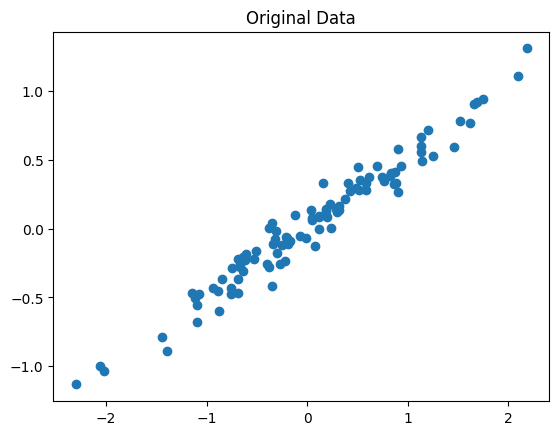
\includegraphics[width=\textwidth]{images/ex3task1-1-1.png}
        \caption{Dataset Plotted}
        \label{fig:Dataset Plotted}
    \end{subfigure}
    \begin{subfigure}[b]{0.45\textwidth}
        \centering
        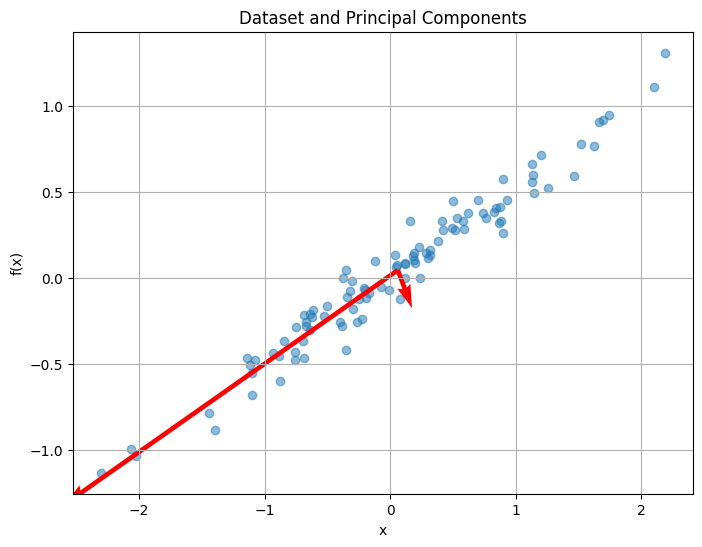
\includegraphics[width=\textwidth]{images/ex3task1-1-2.png}
        \caption{Dataset and Principal Components Plotted}
        \label{fig:Dataset and Principal Components Plotted}
    \end{subfigure}
    \caption{PCA on 2D Dataset}
    \label{fig:part1}
\end{figure}

What we learned from the results of PCA (see figure \ref{fig:part1}).
    \begin{itemize}
        \item This data appears linear and exhibits similar scale.
        \item There are a few data points that are far from the main cluster of data, particularly on the upper right side of the plot. These may be outliers that could potentially influence the PCA.
        \item  The longer red line points in the direction of the first principal component. This is the direction of greatest variance in the dataset. In PCA, this component would capture the most information about the data's structure. The shorter red line is the second principal component, it is orthogonal (at a right angle) to the first. It accounts for the next highest variance in the dataset and is uncorrelated with the first component. 
        \item The PCA seems to be centered around the mean (not necessarily at zero), suggesting that the data has been mean-centered before the PCA was performed.
    \end{itemize}
 

\item \textbf{Part 2:} \\
In Part 2, we analyze an image from the SciPy library. Due to a deprecation warning in SciPy v1.10.0 regarding \texttt{scipy.misc.face}, we have utilized \texttt{scipy.datasets.face} as an alternative. This function retrieves the classic 'face' image, which we use for PCA reconstruction.

\begin{figure}[H]
    \centering
    \begin{subfigure}[b]{0.5\textwidth}
        \centering
        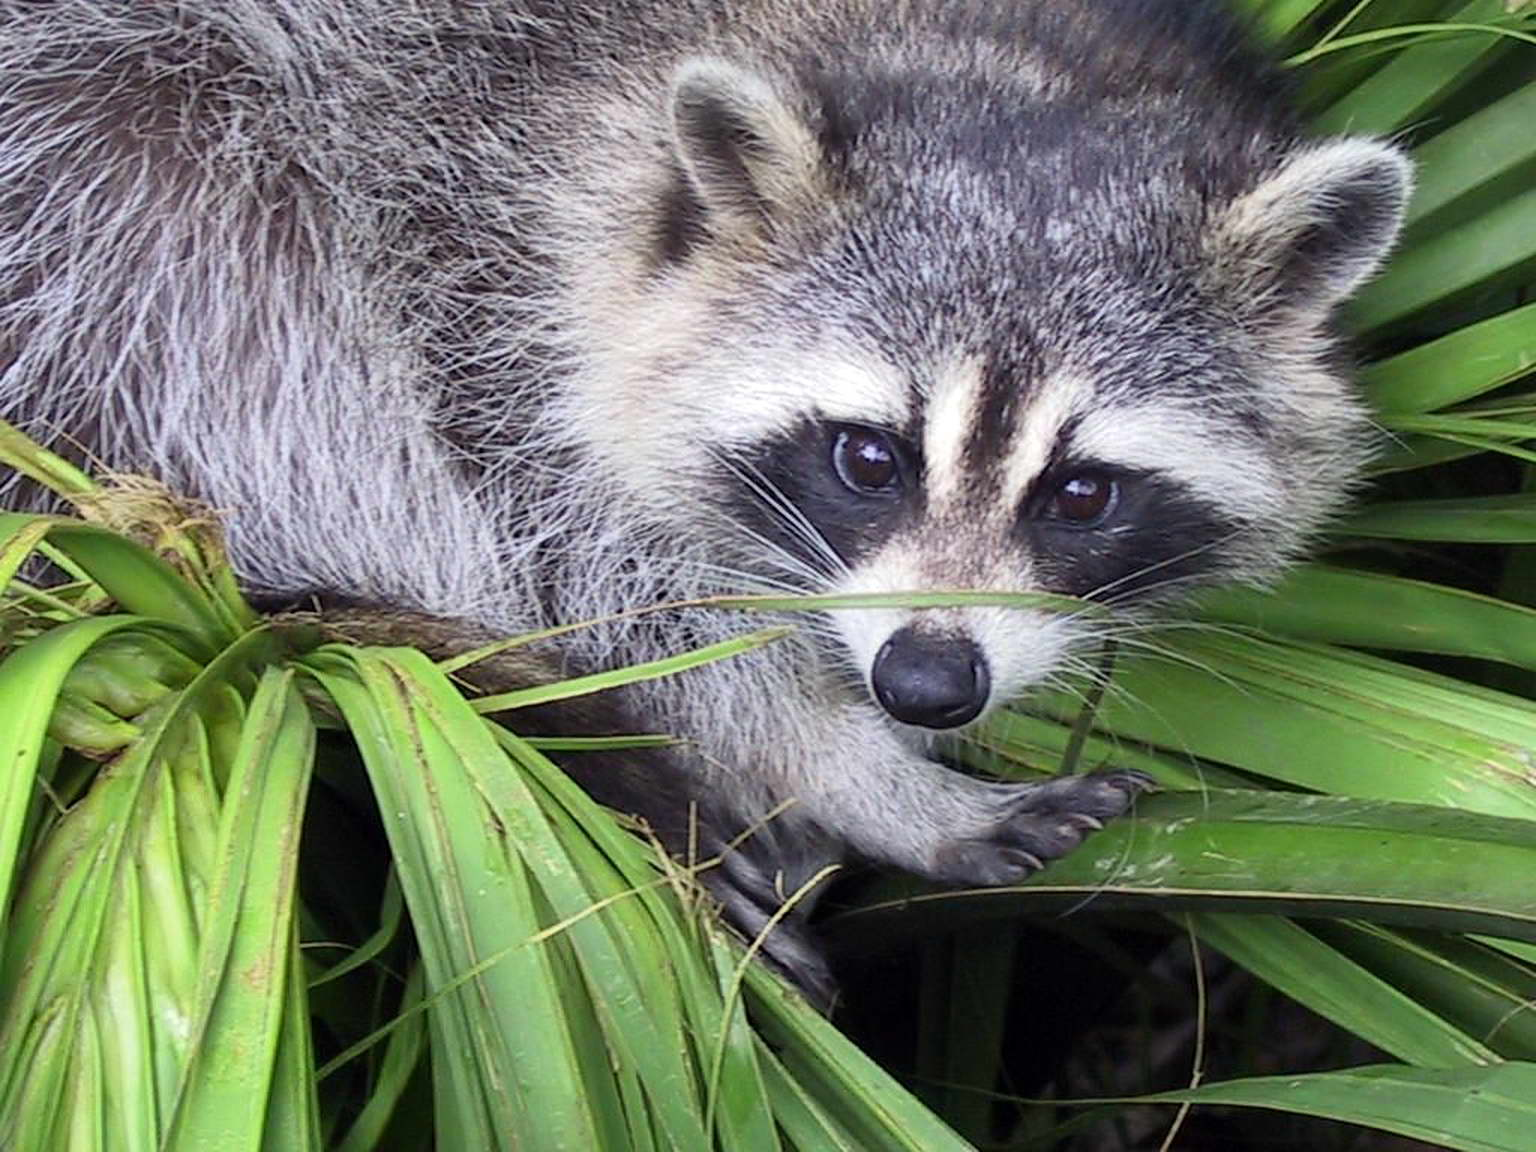
\includegraphics[width=\textwidth]{images/ex3task1-2-1.jpg}
        \caption{Original Image (Before Resizing)}
        \label{fig:original_image}
    \end{subfigure}
    \begin{subfigure}[b]{0.7\textwidth}
        \centering
        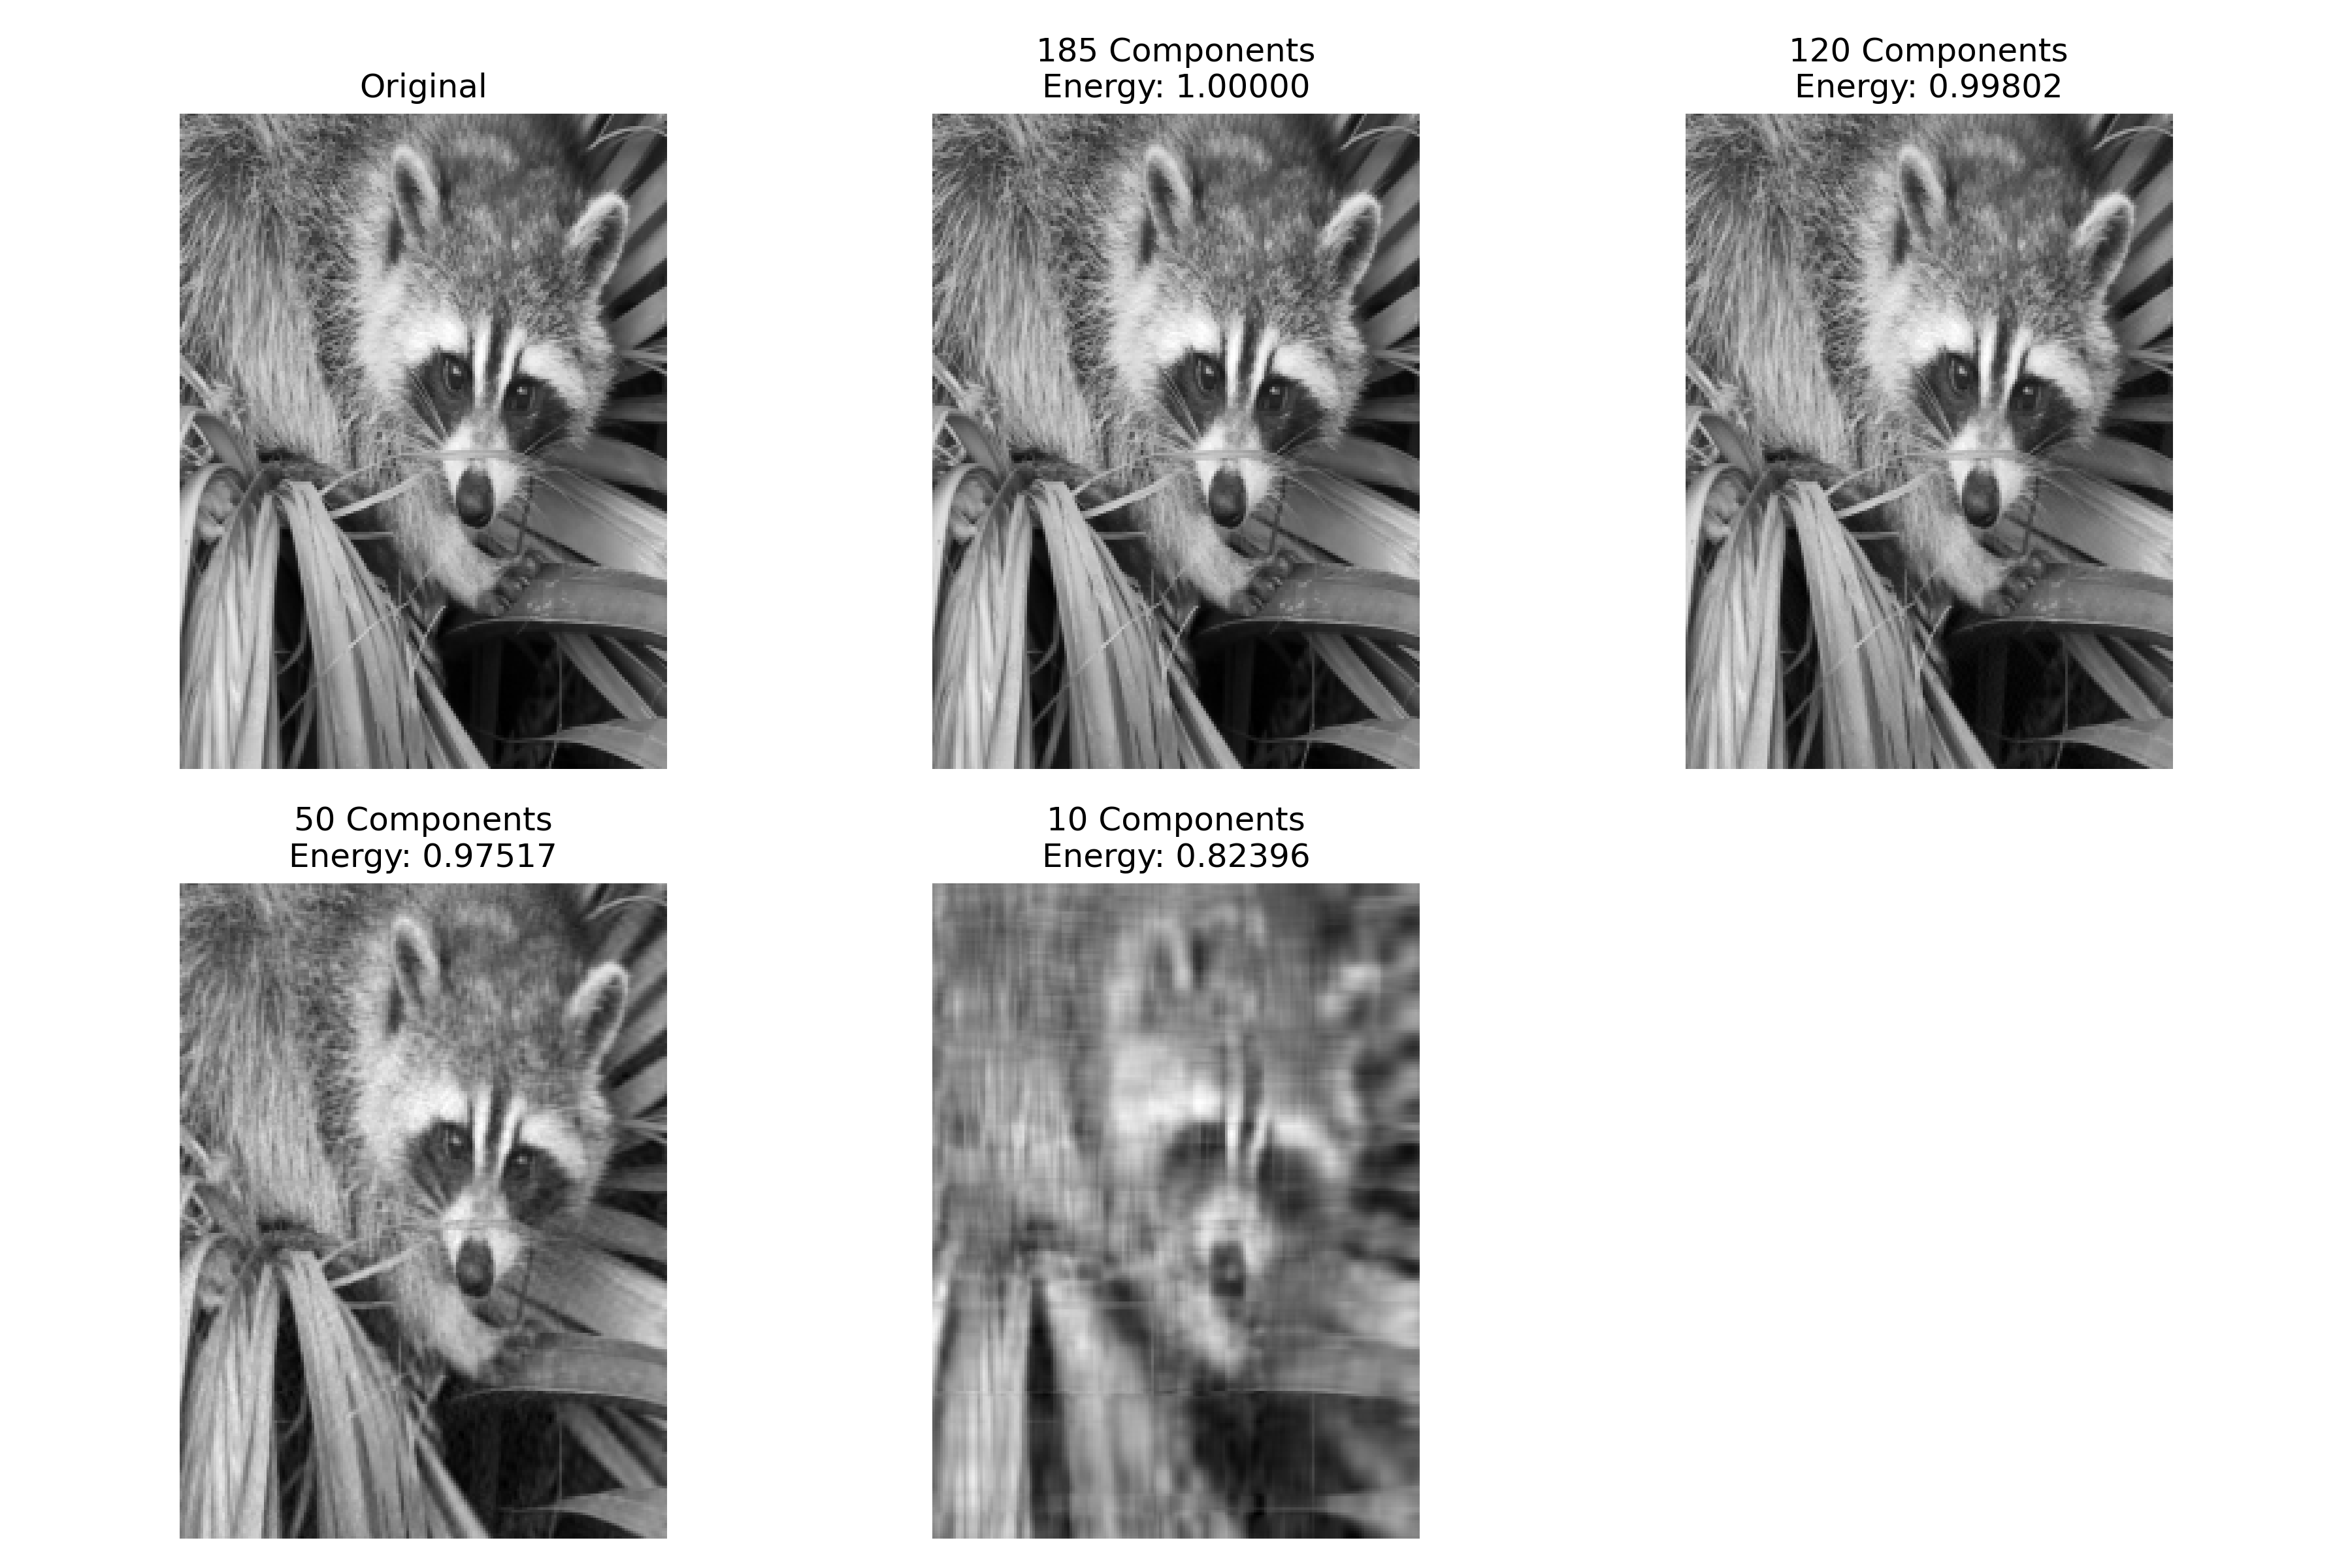
\includegraphics[width=\textwidth]{images/ex3task1-2-2.png}
        \caption{Image Reconstruction Using PCA}
        \label{fig:pca_reconstruction}
    \end{subfigure}
    \caption{PCA on Image Data}
    \label{fig:part2}
\end{figure}

The image dimensions are adjusted to a width of 249 pixels (x-axis) and a height of 185 pixels (y-axis), aligning with the conventional Cartesian coordinate system where 'x' represents the horizontal axis (number of columns) and 'y' represents the vertical axis (number of rows). We then apply Principal Component Analysis (PCA) to this resized image and reconstruct it using varying numbers of principal components. This process allows us to examine the impact of different component counts on the quality of the reconstructed image.


In Figure \ref{fig:part2}, the original image is displayed alongside its PCA reconstructions with varying numbers of components. As the number of components decreases, the clarity of the reconstruction correspondingly diminishes. Retaining all 185 components, which match the image's column count, maintains most of the image's variance. Analysis of the variance captured by different numbers of components reveals that 120 components account for 99.802\% of the variance, 50 components for 97.517\%, and 10 components for 82.396\%.

% P2: At what number is the information loss visible?
Information loss becomes visibly evident when the number of components falls well below the total column count of 185. Particularly, with 50 components, where 97.517\% of the variance is explained, the degradation in detail and sharpness starts to be perceptible.

% P2: At what number is the energy lost through truncation smaller than 1\%?
The truncation's energy loss is less than 1\% when 120 components are used since they explain 99.802\% of the variance, indicating a minimal remainder of energy loss.

What we learned from the results of PCA.
    \begin{itemize} 
    \item This illustrates the inherent compromise in PCA, there's a balance between the accuracy of the reconstructed data and the number of principal components used. A reduction in components leads to a more abstract and less detailed reconstruction, trading precision for reduced dimensionality. Comparing reconstructions with varying numbers of PCs can aid in grasping the data's complexity and in determining the necessary number of PCs to capture the image(data)'s essential patterns.
    \end{itemize}



% \begin{figure}[H]\ContinuedFloat
%     \centering
%     \begin{subfigure}[b]{0.7\textwidth}
%         \centering
%         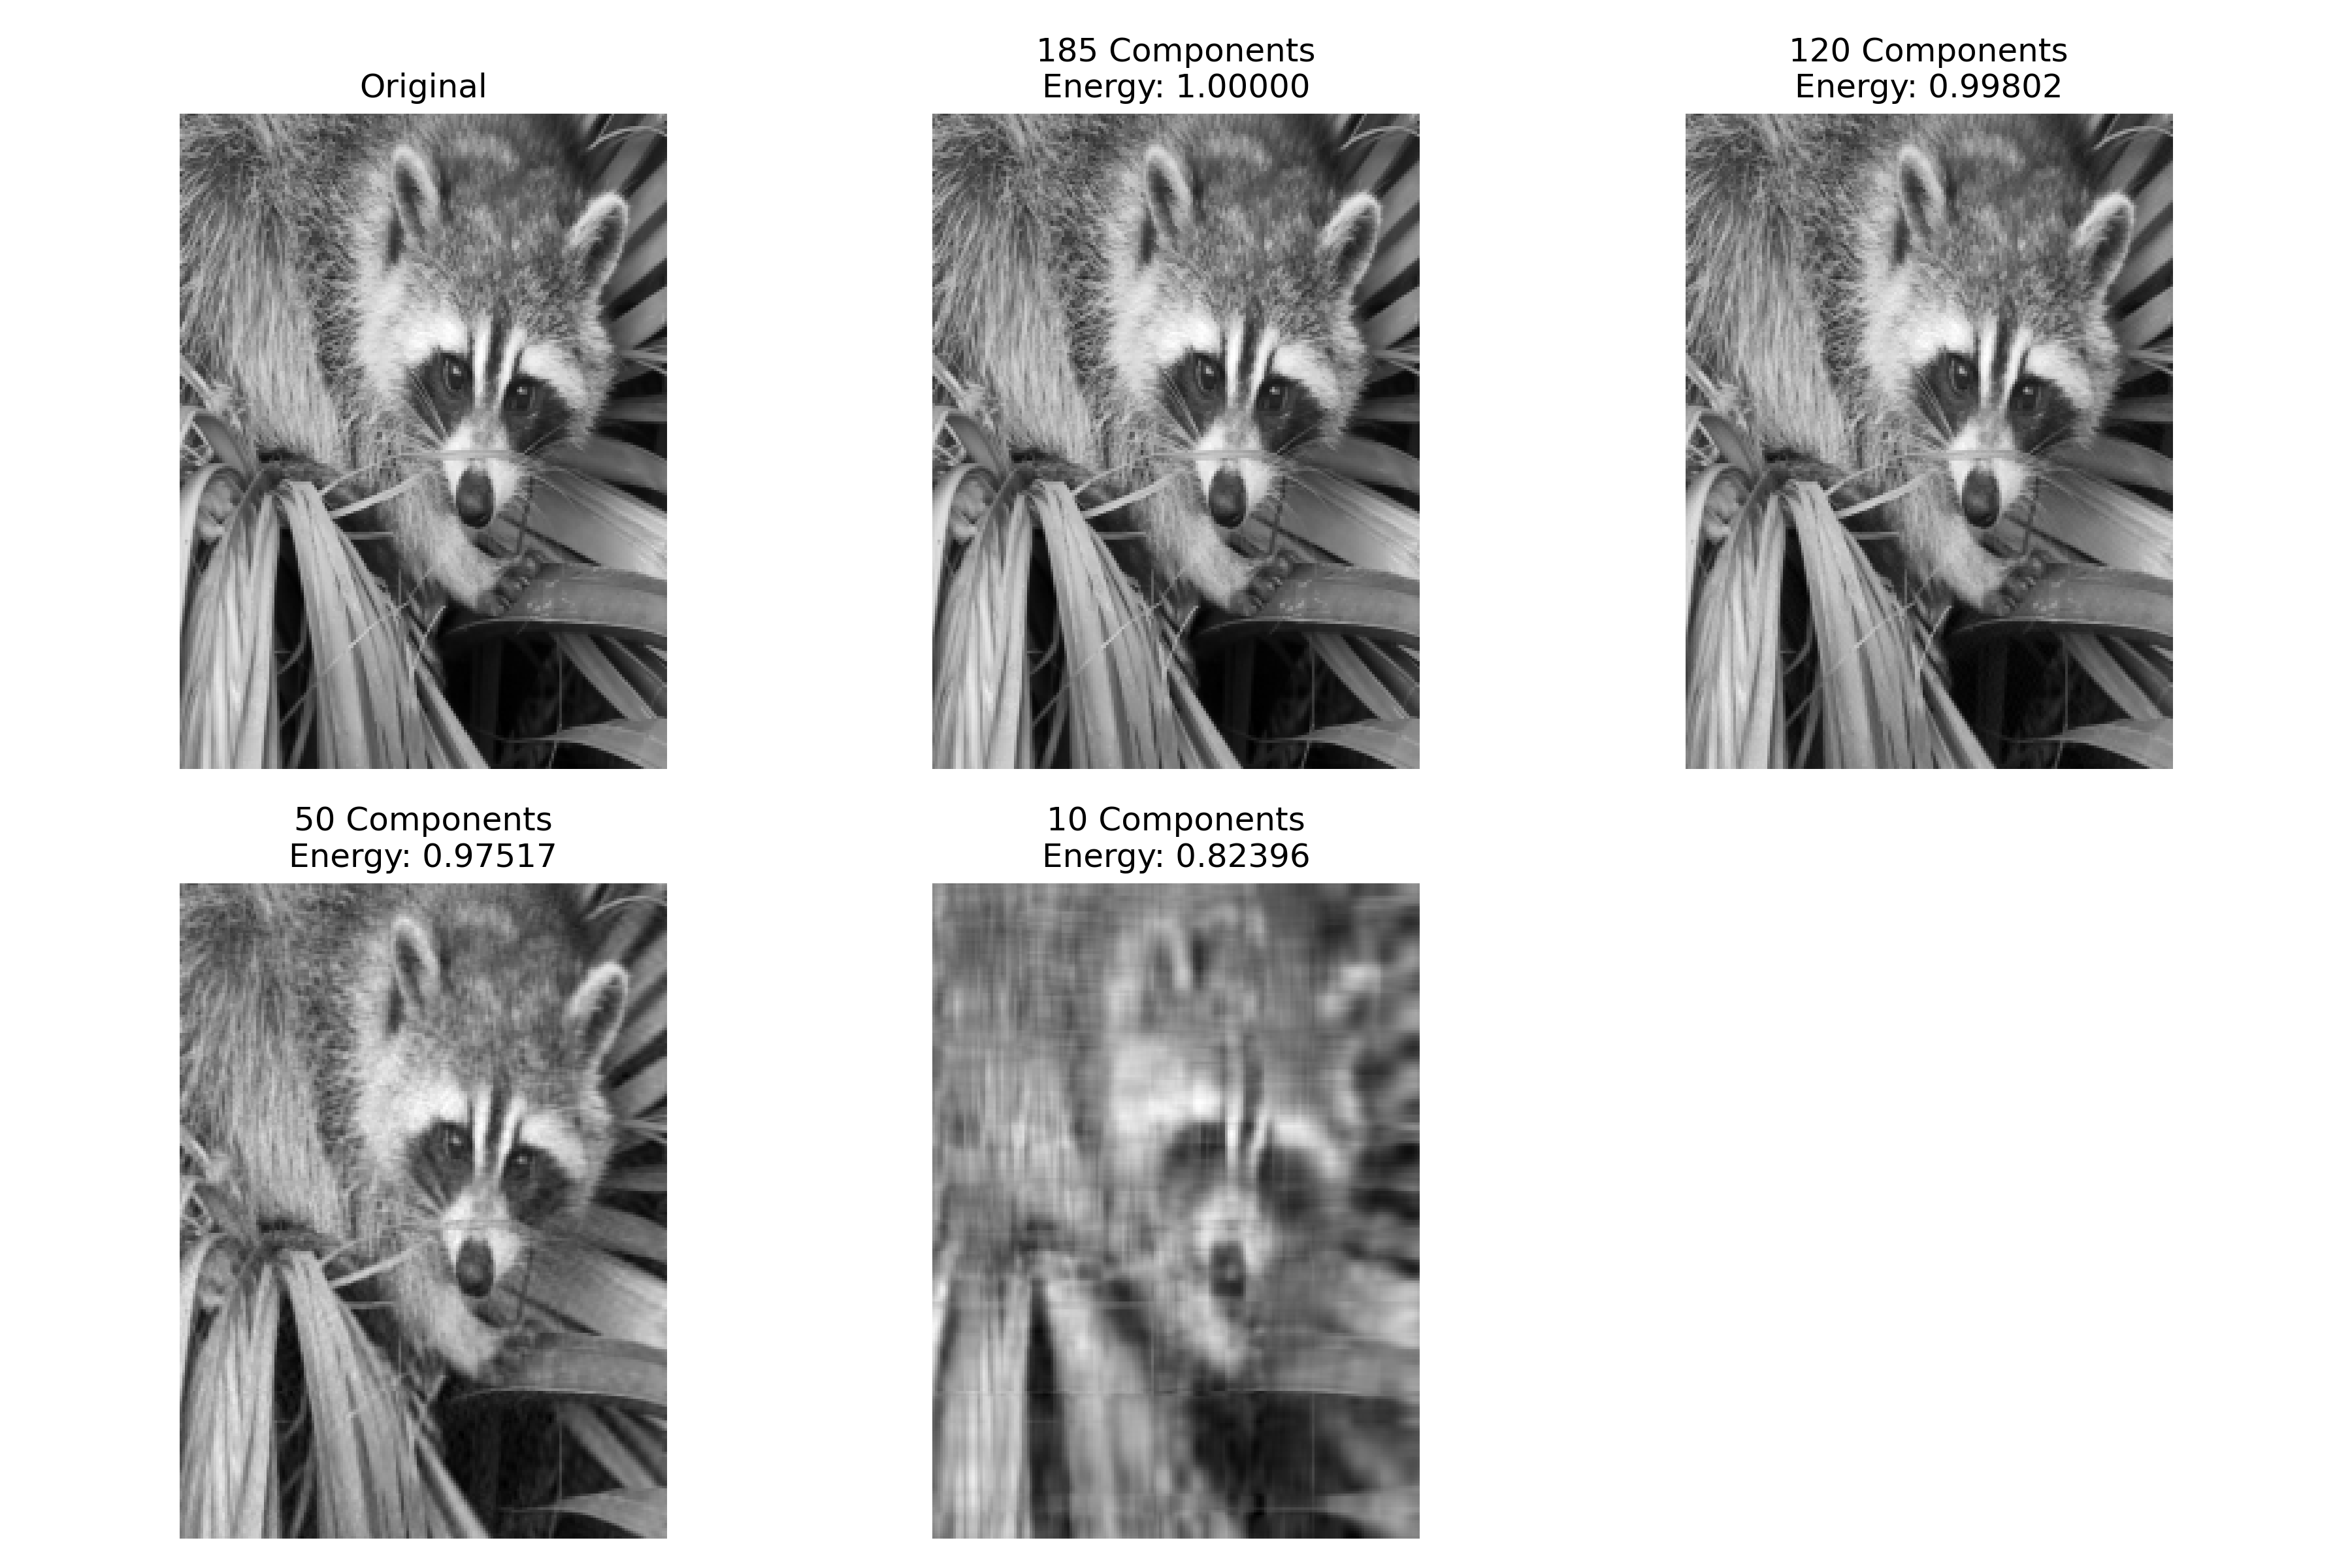
\includegraphics[width=\textwidth]{images/ex3task1-2-2.png}
%         \caption{Image Reconstruction Using PCA}
%         \label{fig:pca_reconstruction}
%     \end{subfigure}
%     \caption{PCA on Image Data}
%     \label{fig:part22}
% \end{figure}





\item \textbf{Part 3:} \\
Part 3 involves analyzing the trajectory data of 15 people. We specifically focus on visualizing the paths of the first two pedestrians in a 2D space.

\begin{figure}[H]
    \centering
    \begin{subfigure}[b]{0.8\textwidth}
        \centering
        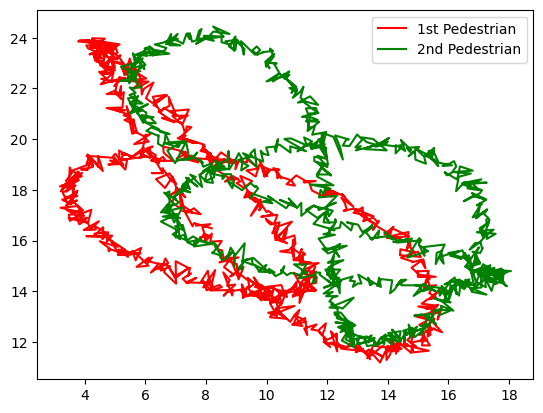
\includegraphics[width=\textwidth]{images/ex3task1-3-1.png}
        
        \label{fig:original_trajectory_pedestrians}
    \end{subfigure}
    \caption{Original Trajectory of Pedestrian 1,2}
    \label{fig:part3-1}
\end{figure}


The trajectories in figure \ref{fig:part3-1} exhibit circular movement patterns and show the raw tracking data, which is replete with noise and jagged lines, capturing all the variance but lacking the detail needed to fully describe the complexity of the pedestrians' paths.

\begin{figure}[H]
    \centering
    \begin{subfigure}[b]{0.45\textwidth}
        \centering
        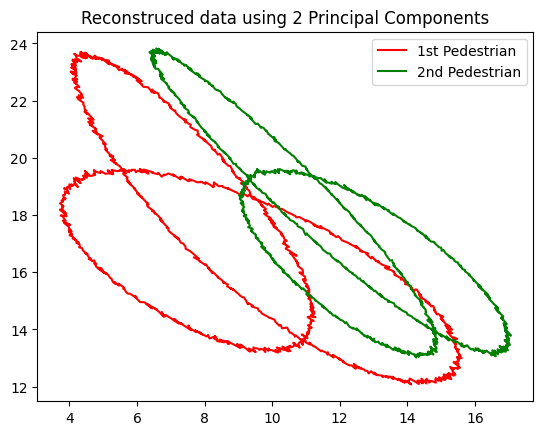
\includegraphics[width=\textwidth]{images/ex3task1-3-2.png}
        \caption{Trajectory of Pedestrian 1,2 with 2 components}
        \label{fig:Trajectory of Pedestrian 1,2 with 2 component3}
    \end{subfigure}
    \begin{subfigure}[b]{0.45\textwidth}
        \centering
        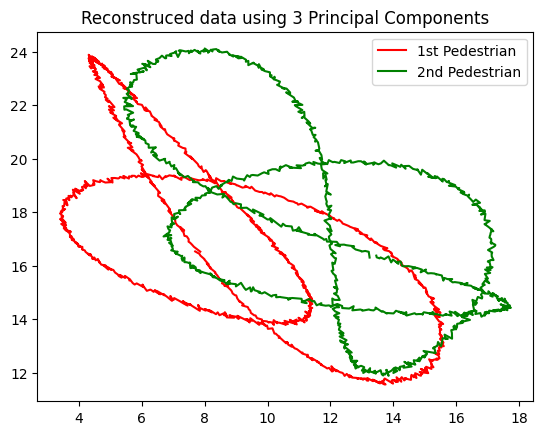
\includegraphics[width=\textwidth]{images/ex3task1-3-3.png}
        \caption{Trajectory of Pedestrian 1,2 with 3 component}
        \label{fig:Trajectory of Pedestrian 1,2 with 3 component}
    \end{subfigure}
    \caption{PCA on Pedestrian Trajectories}
    \label{fig:part3-2}
\end{figure}

In figure \ref{fig:Trajectory of Pedestrian 1,2 with 2 component3}, PCA with 2 components is shown. The trajectories are still distinguishable but have lost some detail compared to the multi-component reconstruction. The paths are broader and less precise, indicating that the third principal component may have contained information that contributed to a more nuanced description of the motion. The variance explained by each component is [0.47320404, 0.37601352], with an overall explained variance of approximately 0.849. Given the complex nature of the trajectories, two components are insufficient to capture the majority of the dataset's energy. The explained variance with 2 components is below 90\%.

Consequently, we are considering using more than 2 components, specifically 3 components, as depicted in figure \ref{fig:Trajectory of Pedestrian 1,2 with 3 component}. The circular patterns in the data introduce complexity that requires additional dimensions for an accurate representation. To capture more than 90\% of the variance, at least 3 components are necessary, As a result, the 3-component plot shows a fairly smooth and well-defined trajectory for both pedestrians. The use of three principal components suggests that this is a higher-fidelity reconstruction of their movement, retaining more detail of the motion paths. This is also evidenced by the increase in explained variance to approximately 0.997 with 3 components. the variance explained is [0.47320404, 0.37601352, 0.14791464], resulting in an overall explained variance of approximately 0.997.

What we learned from the results of PCA.

\begin{itemize}
    \item PCA is used to reduce the dimensionality of data, which could be very high-dimensional if it includes many tracked points or is sampled at a high frequency. This leads to noise filtering, as higher-order components may correspond to less significant movements or noise. By utilizing fewer principal components, the data can be compressed, retaining the most critical information which might suffice for some applications such as basic movement analysis or pattern recognition.
    \end{itemize}

\end{itemize}


% time estimate 
The development and implementation of the PCA code took approximately 2 hours, with a significant portion of this time dedicated to the intricacies of PCA itself. The volumne of data itself was relatively small, so implementing it did not take significant time. 

%Accuracy Considerations 
Accuracy for model is commonly evaluated using metrics such as Mean Squared Error (MSE). However, the nature of our datasets doesn't comply with model accuracy. For the first dataset, which is two-dimensional, employing PCA does not reduce dimensionality but rather linearizes the data. Given its limited variable count, conventional model evaluation techniques are not applicable. The second dataset, being an image, and the third dataset, consisting of pedestrian's trajectory data, also have characteristics that limit the suitability of standard modeling approaches. 

Therefore, we have opted to consider the 'energy' retained in the principal components as an alternative measure of accuracy for these datasets. It's essential to understand that while this method offers insight into the variance captured by PCA, it does not provide a comprehensive assessment of model accuracy in the same manner as error metrics like MSE. Moreover, it is important to recognize that applying PCA does not necessarily improve MSE or other error metrics, as the effectiveness of PCA largely depends on the specific characteristics and requirements of the data being analyzed.

% what we learned
% We learned about PCA.
% Data. 

% Verbose discussion of the results in the report?
% Code: modular, concise, well documented?


\end{task}

\begin{task}{2, Implementation of the SpectralEmbedding method}
% Part 1: Estimate the linear vector field that was used to generate the points x1 from the points x0.
% Part 2: Solve the linear system and compute the mean squared error.
% Part 3: Choose the initial point (10, 10) and solve the system.
% Part 3: Visualize the trajectory as well as the phase portrait.

For this task, we are given two linear vectorfield datasets with 1000 points each. Each row represents a data point, providing the initial position $x_0^{(k)}$ and the corresponding final position $x_1^{(k)}$. The given datasets are plotted in figure \ref{fig:task2data}.

    \begin{figure}[H]
        \centering
        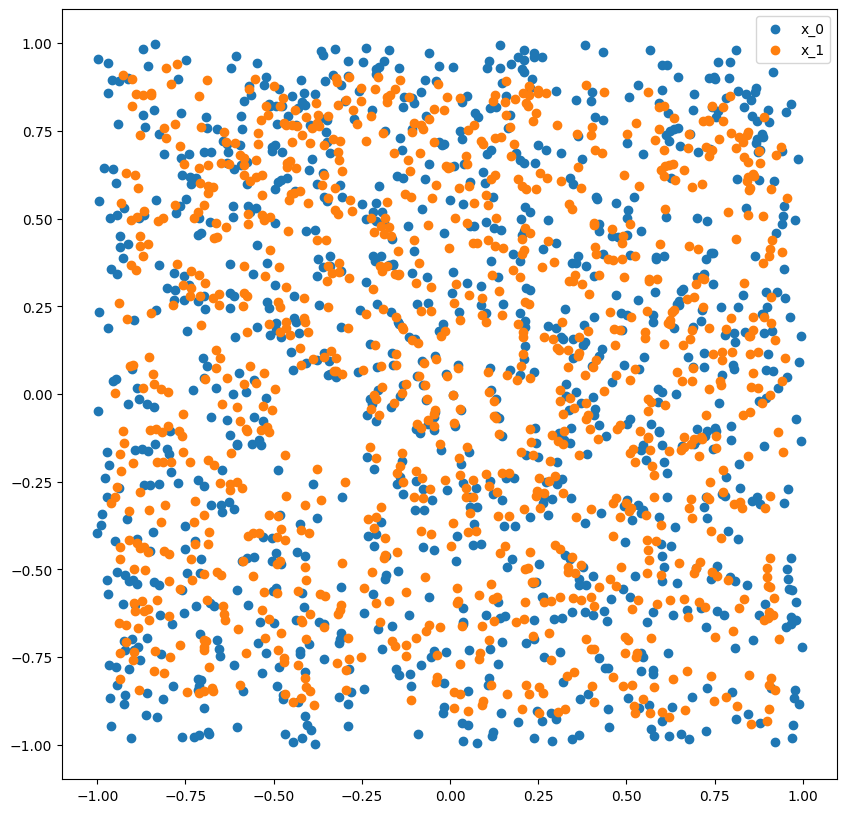
\includegraphics[width=0.5\linewidth]{images/Ex5task2_data.png}
        \caption{Dataset for task 2}
        \label{fig:task2data}
    \end{figure}

\begin{itemize}
    \item \textbf{Part 1:} For this task, we have to estimate the linear vector field that was used to generate the points {$x_1$} from the points {$x_0$}. Using the finite difference formula with a time step ($\Delta$t=0.1), the vector v\_hat is estimated at each point x$_0^{(k)}$. This captures the rate of change in the system. We then employed the least square solution to approximate the matrix A. This matrix captures the linear transformation between the initial positions and the final vectors.

    \item \textbf{Part 2:} For this task, we have to estimate the linear vector field and evaluate the accuracy of our estimated matrix A. We used the \texttt{solve\_ivp} function to simulate the linear system for each initial point $x^{(k)}_0$ up to the specified end time T$_{end}$ = $\Delta$t = 0.1. We obtained a mean squared error of \texttt{0.0030599} providing a measure of the average integration error. The approximated data after $\Delta{t}=0.1$ is shown in figure \ref{fig:task2data01}.
    
    \begin{figure}[H]
        \centering
        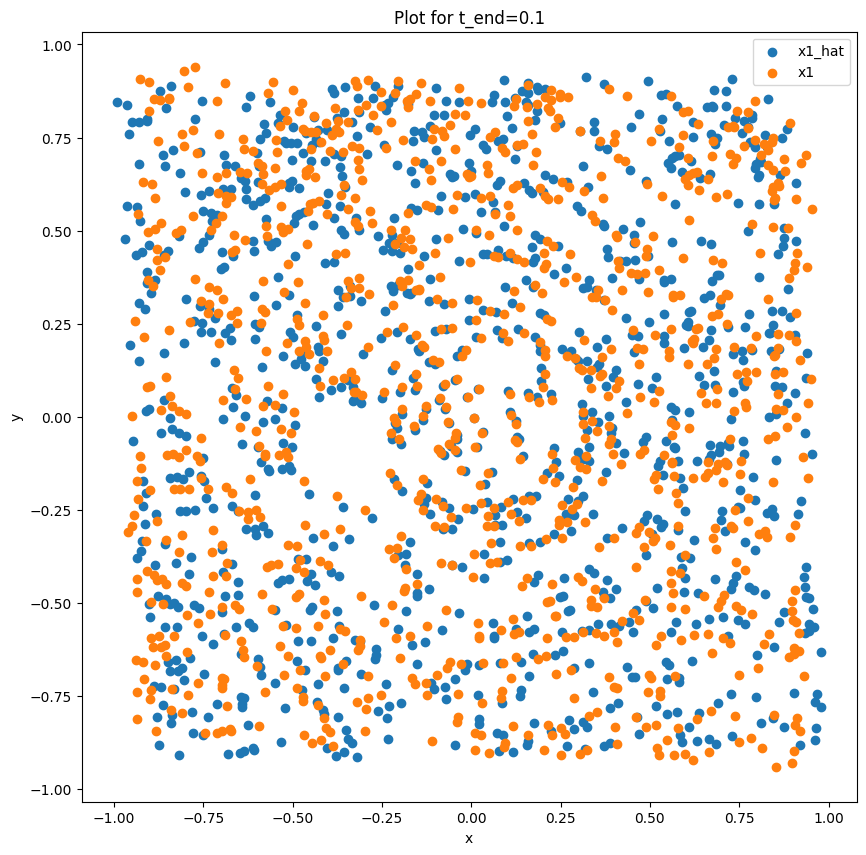
\includegraphics[width=0.6\linewidth]{images/Ex5task2_01.png}
        \caption{Approximated data after $\Delta{t}=0.1$}
        \label{fig:task2data01}
    \end{figure}

    \item \textbf{Part 3:} For this task, we first plot the phase portrait of our system and we can see that all values converge to the origin, or in other words we can say that this is the steady point of the system.\\
    We then choose an initial point (10,10), which is far outside our initial data, and solve the linear system with our approximated matrix $A\_approximated$ for a large time T$_{end}=100$. We can see that point follows the phase portrait of our system and converges to the steady point at origin.\\
    The phase portrait along with the trajectory can be seen in figure \ref{fig:task2final}.

    \begin{figure}[H]
        \centering
        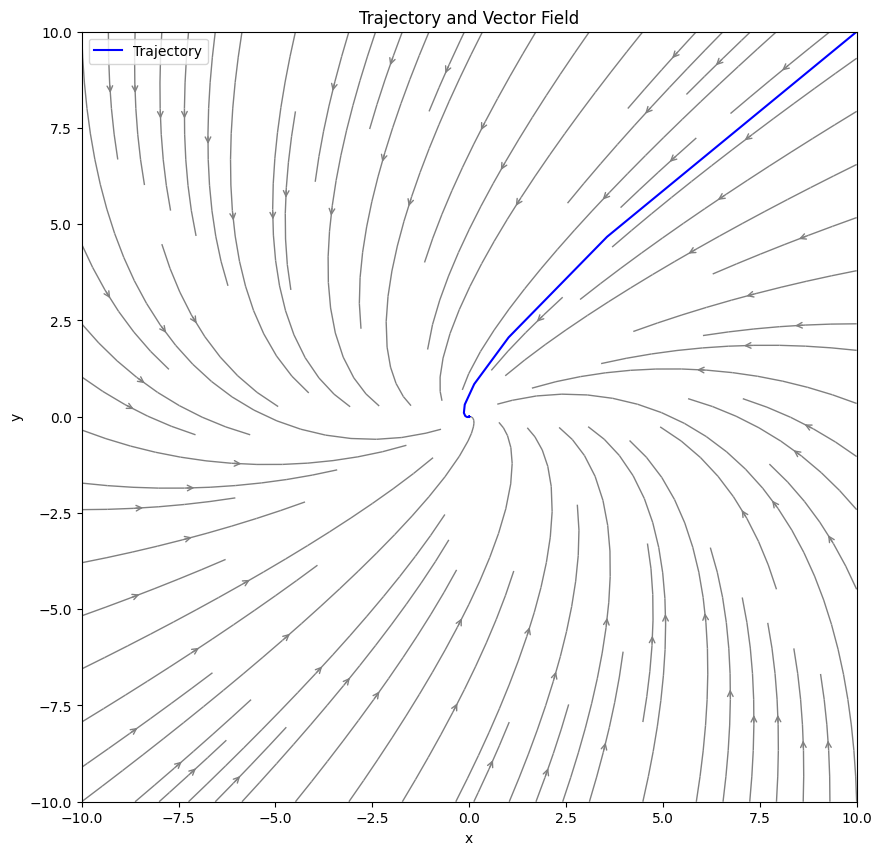
\includegraphics[width=0.6\linewidth]{images/Ex5task2_final.png}
        \caption{Plotted trajectory for $T_{end}=100$ and initial point [10,10]}
        \label{fig:task2final}
    \end{figure}
\end{itemize}
\end{task}

\begin{task}{3, Description of the libraries used}
Task 3 explores the option of using a Variational Autoencoder (VAE). In order to train our first model, we will use the MNIST dataset \cite{deng2012mnist} containing 60,000 training samples as well as 10,000 test samples of handwritten numbers and normalise the pixel values between 0 and 1. The task specifies what the model should look like: 

\begin{itemize}
    \item two-dimensional latent space
    \item multivariate diagonal Gaussian distribution as approximate posterior $q_\phi(z \vert x)$
    \item Encoder (outputs the mean and standard deviation of $q_\phi(z \vert x)$): 
    \begin{itemize}
        \item 2 hidden layers with 256 units each and ReLU activation functions
        \item multivariate diagonal Gaussian distribution as likelihood $p_\theta(x \vert z)$
    \end{itemize}
    \item Decoder (outputs only the mean of $p_\theta(x \vert z)$):
    \begin{itemize}
        \item 2 hidden layers with 256 units each and ReLU activation functions
        \item standard deviation for the decoder distribution as one floating-point, trainable variable
    \end{itemize}
    \item multivariate diagonal standard normal distribution as the prior $p(z)$
\end{itemize}

Additionally, the Adam optimiser is used with a learning rate of 0.001, as well as a batch size of 128 for training. The libraries used in our code are depicted in table \ref{tab:vae-libraries} together with the functionalities that we utilised.  \\

\begin{table}[hbt!]
\centering
%\resizebox{\textwidth}{!}
{%
\begin{tabular}{|l|l|}
\hline
Tensorflow \cite{tensorflow2015-whitepaper}  & \begin{tabular}[c]{@{}l@{}}download the MNIST dataset\\ \& implement Early Stopping\end{tabular}  \\ \hline
Numpy \cite{harris2020array}    &    generate random samples  from a normal (Gaussian) distribution    \\ \hline
Matplotlib \cite{Hunter:2007} & visualise the constructed and generated images \\ \hline
\end{tabular}%
}
\caption{Libraries and their utilised functions for the task of VAE}
\label{tab:vae-libraries}
\end{table}


\textbf{1. What activation functions should be used for the mean and standard deviation of the approximate posterior and the likelihood and why?} \\

The choice of activation functions for the mean and standard deviation in a VAE is critical due to the properties of Gaussian distributions. For the mean \(\mu\) of the approximate posterior \(q_\phi(z | x)\), a linear activation function is appropriate as the mean can take on any real value. Hence, no activation function, or the identity function, is typically used:

\begin{equation}
\mu = W_{\mu}h + b_{\mu}
\end{equation}

where \(W_{\mu}\) and \(b_{\mu}\) are the weights and biases for the mean, and \(h\) is the output from the last hidden layer of the encoder.

For the standard deviation \(\sigma\), we require an activation function that ensures the output is positive, as the standard deviation must be non-negative. The softplus function is commonly used for this purpose:

\begin{equation}
\sigma = \log(1 + \exp(W_{\sigma}h + b_{\sigma}))
\end{equation}

where \(W_{\sigma}\) and \(b_{\sigma}\) are the weights and biases for the standard deviation.

The softplus function is smooth and gradually increases, avoiding any abrupt changes in the gradient, which benefits the stability of the learning process. Additionally, it closely approximates a ReLU function for large input values, effectively preventing the standard deviation from collapsing to zero.

For the likelihood \(p_\theta(x | z)\), the decoder outputs only the mean, and since the pixel values are normalized between 0 and 1, a sigmoid activation function is used to ensure the output is within this range:

\begin{equation}
\hat{x} = \sigma(W_{\hat{x}}z + b_{\hat{x}})
\end{equation}

where \(\sigma(\cdot)\) is the sigmoid function, ensuring that the reconstructed input \(\hat{x}\) is in the range \([0, 1]\), corresponding to the normalized pixel values.\\


\textbf{2. What might be the reason if we obtain good reconstructed but bad generated digits?} \\

There exist multiple possible reasons for the VAE to produce badly generated digits like learning rate, training duration, or loss function. However, it is apparent that the latent space of our model is very small. This can result in the model not having enough capacity to represent the diversity of the data during generation. Because of this, we will increase the latent space in part 5 of this task. \\

% Train the VAE (training set) and do the following experiments (test set) after the 1st epoch, the 5th epoch, the 25th epoch, the 50th epoch, and after the optimisation converged:
\textbf{3. Train the VAE} \\

In question 3, we train the VAE. After the 1st, 5th, 25th, and 50th epoch, we will plot the latent representation, plot reconstructed digits, and plot generated digits. Additionally, we do the same after convergence. To determine when the optimisation converges, we make use of Early Stopping which monitors \texttt{val\_loss} and uses patience of 5. The exact point of convergence will differ since the VAE does not work deterministically. In the figures we provided in the report, Early Stopping happened after epoch 55. \\

\textbf{3.1. Plot the latent representation} \\

We have our results of transformation of the latent space of a Variational Autoencoder (VAE) as it is trained over multiple epochs. The plots show the latent representations of a test dataset, where each point corresponds to a high-dimensional data instance compressed into two latent dimensions for visualization purposes. The color indicates class labels, which are not used during the unsupervised training of the VAE but are shown here to demonstrate the clustering capability of the model.

Subplot \ref{fig:latentRep1} depicts the latent space after 1 epoch of training. The data points are largely overlapped, indicating that the VAE has not yet learned to separate the different classes effectively in the latent space.

Subplot \ref{fig:latentRep5} shows the latent space after 5 epochs. The beginnings of cluster formation can be observed, with the VAE starting to distinguish between classes, although considerable overlap still exists.

Subplot \ref{fig:latentRep25} represents the latent space after 25 epochs. The clusters are more defined, showing that the VAE has improved in mapping similar data points (from the same class) closer together in the latent space while separating different classes.

Subplot \ref{fig:latentRep50} presents the latent space after 50 epochs. The clusters are well-defined and mostly non-overlapping, illustrating that the VAE is now capable of organizing the data in a way that similar instances are located in proximity to each other, forming distinct clusters corresponding to the different classes. This suggests a matured learning where the encoder part of the VAE has developed a more structured understanding of the data.
% explanation for latent representation

\begin{figure}[H]
    \centering
    \begin{subfigure}[b]{0.45\textwidth}
        \centering
        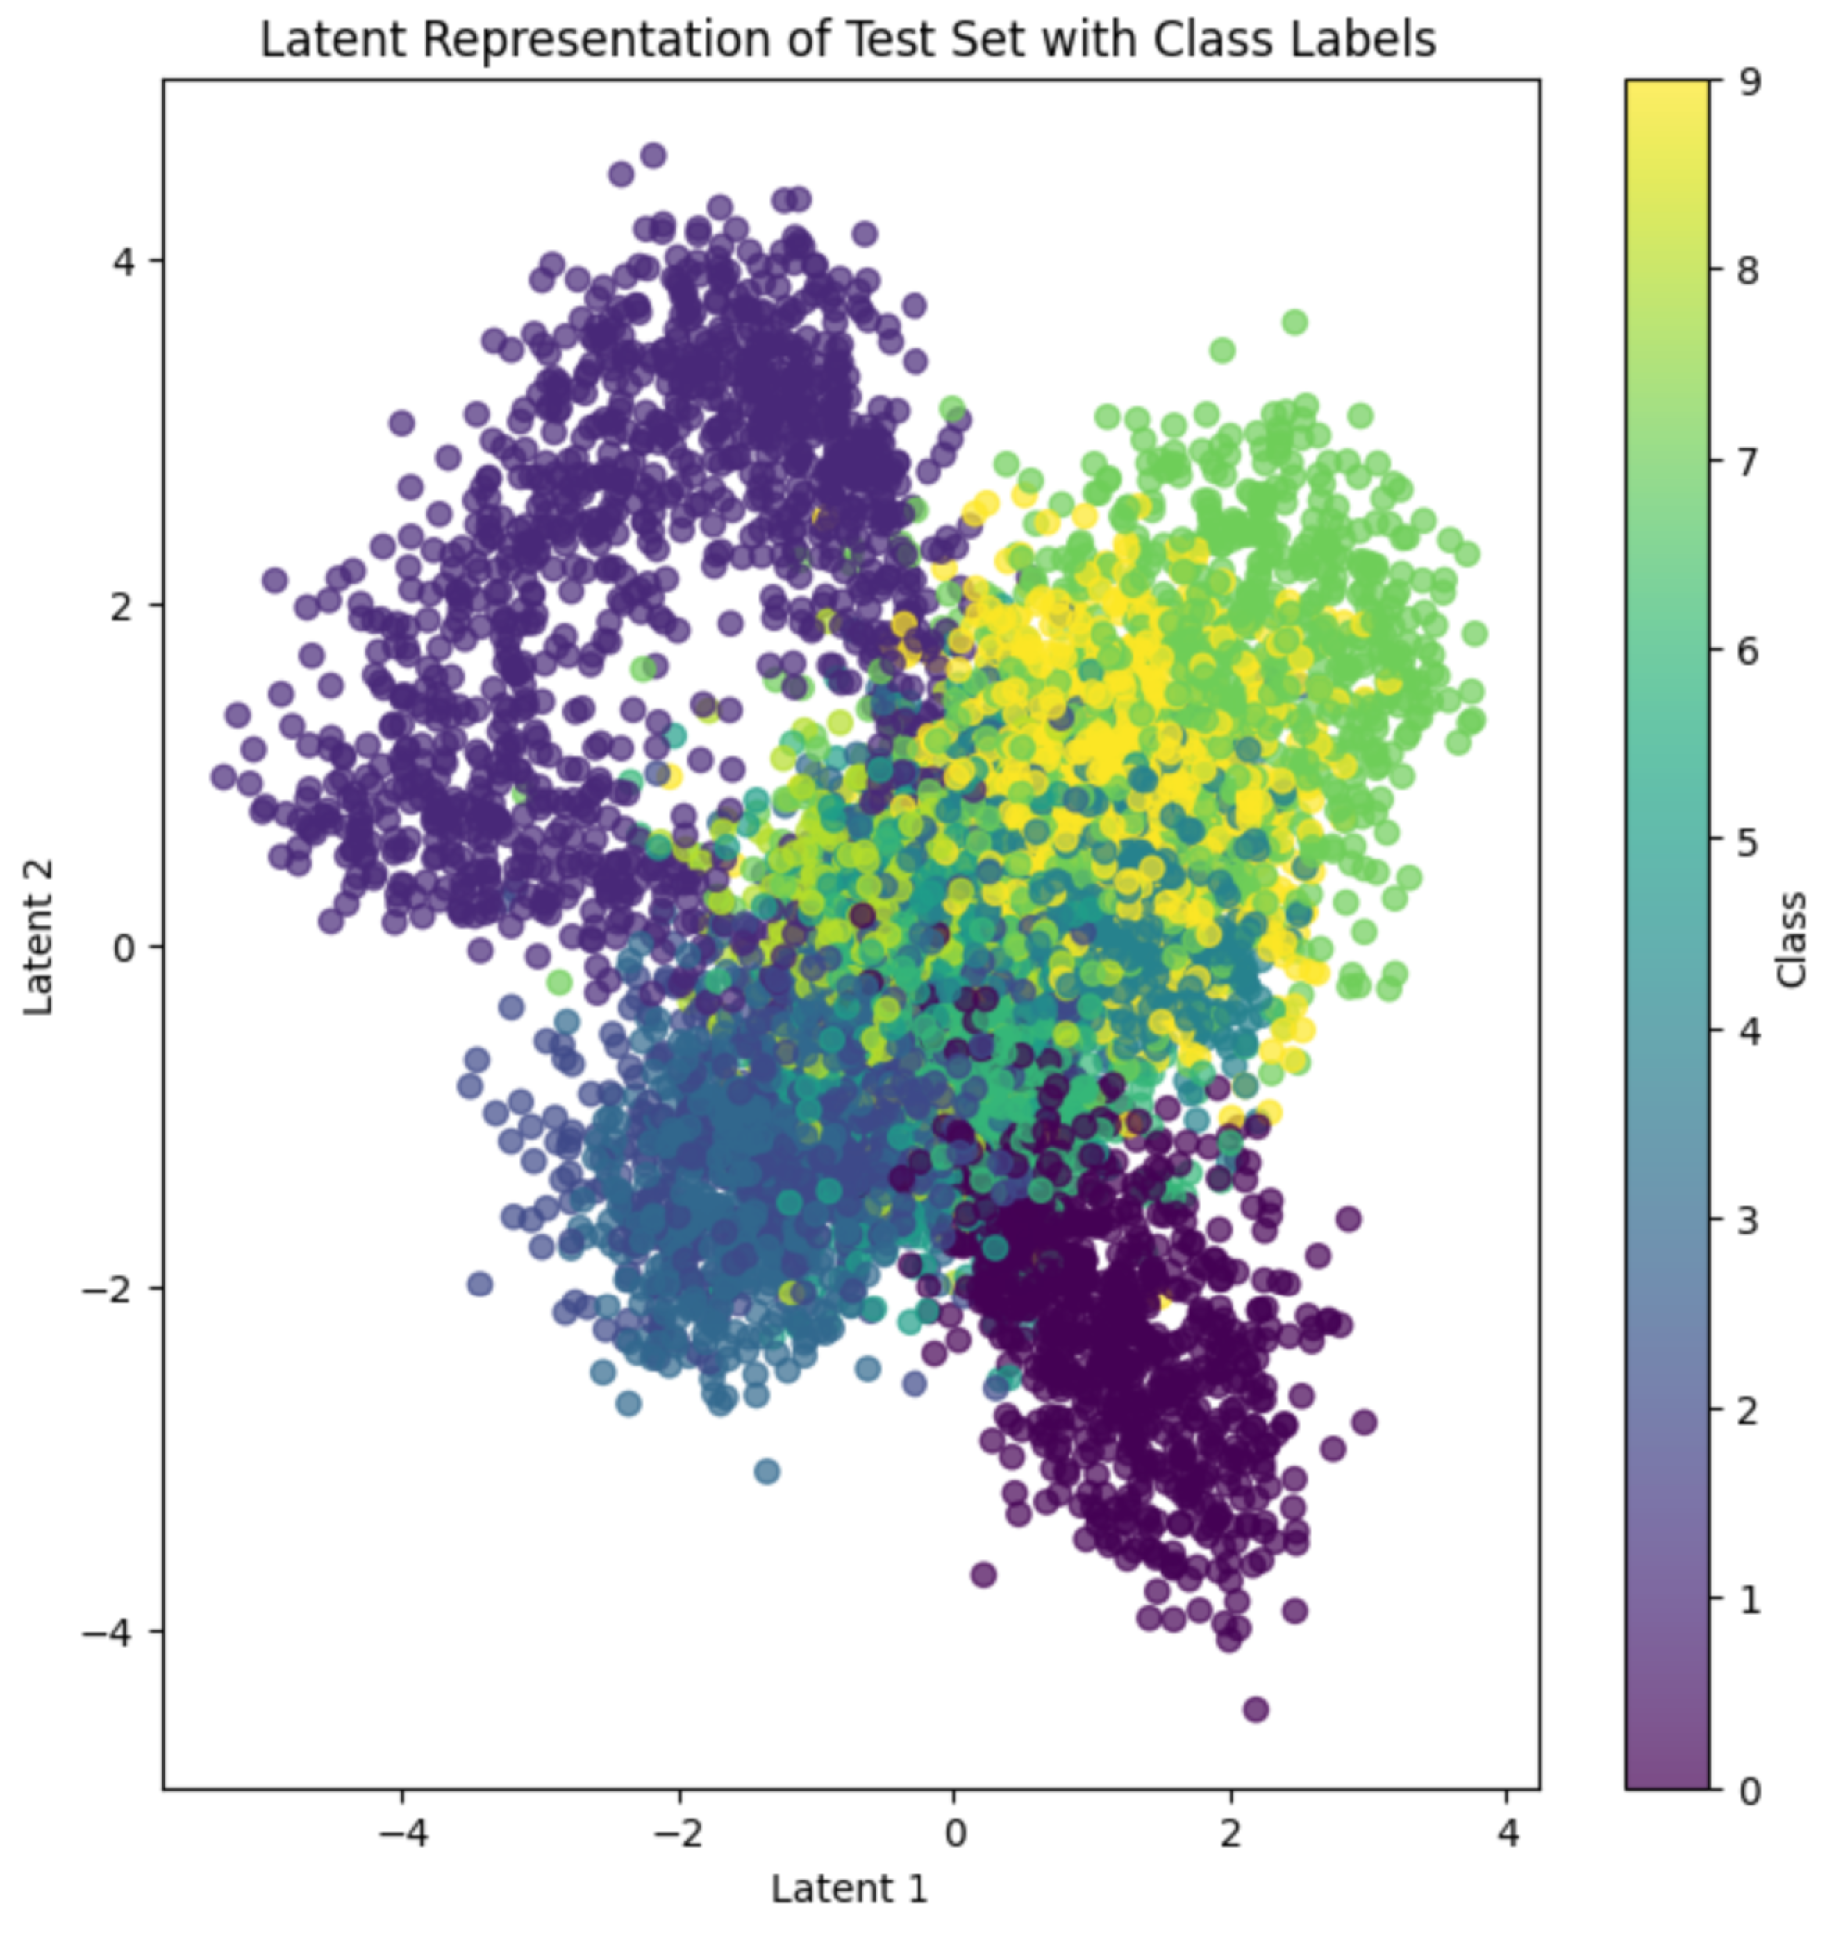
\includegraphics[width=\textwidth]{images/3-latentRep1.png}
        \caption{1 epoch}
        \label{fig:latentRep1}
    \end{subfigure}
    \begin{subfigure}[b]{0.45\textwidth}
        \centering
        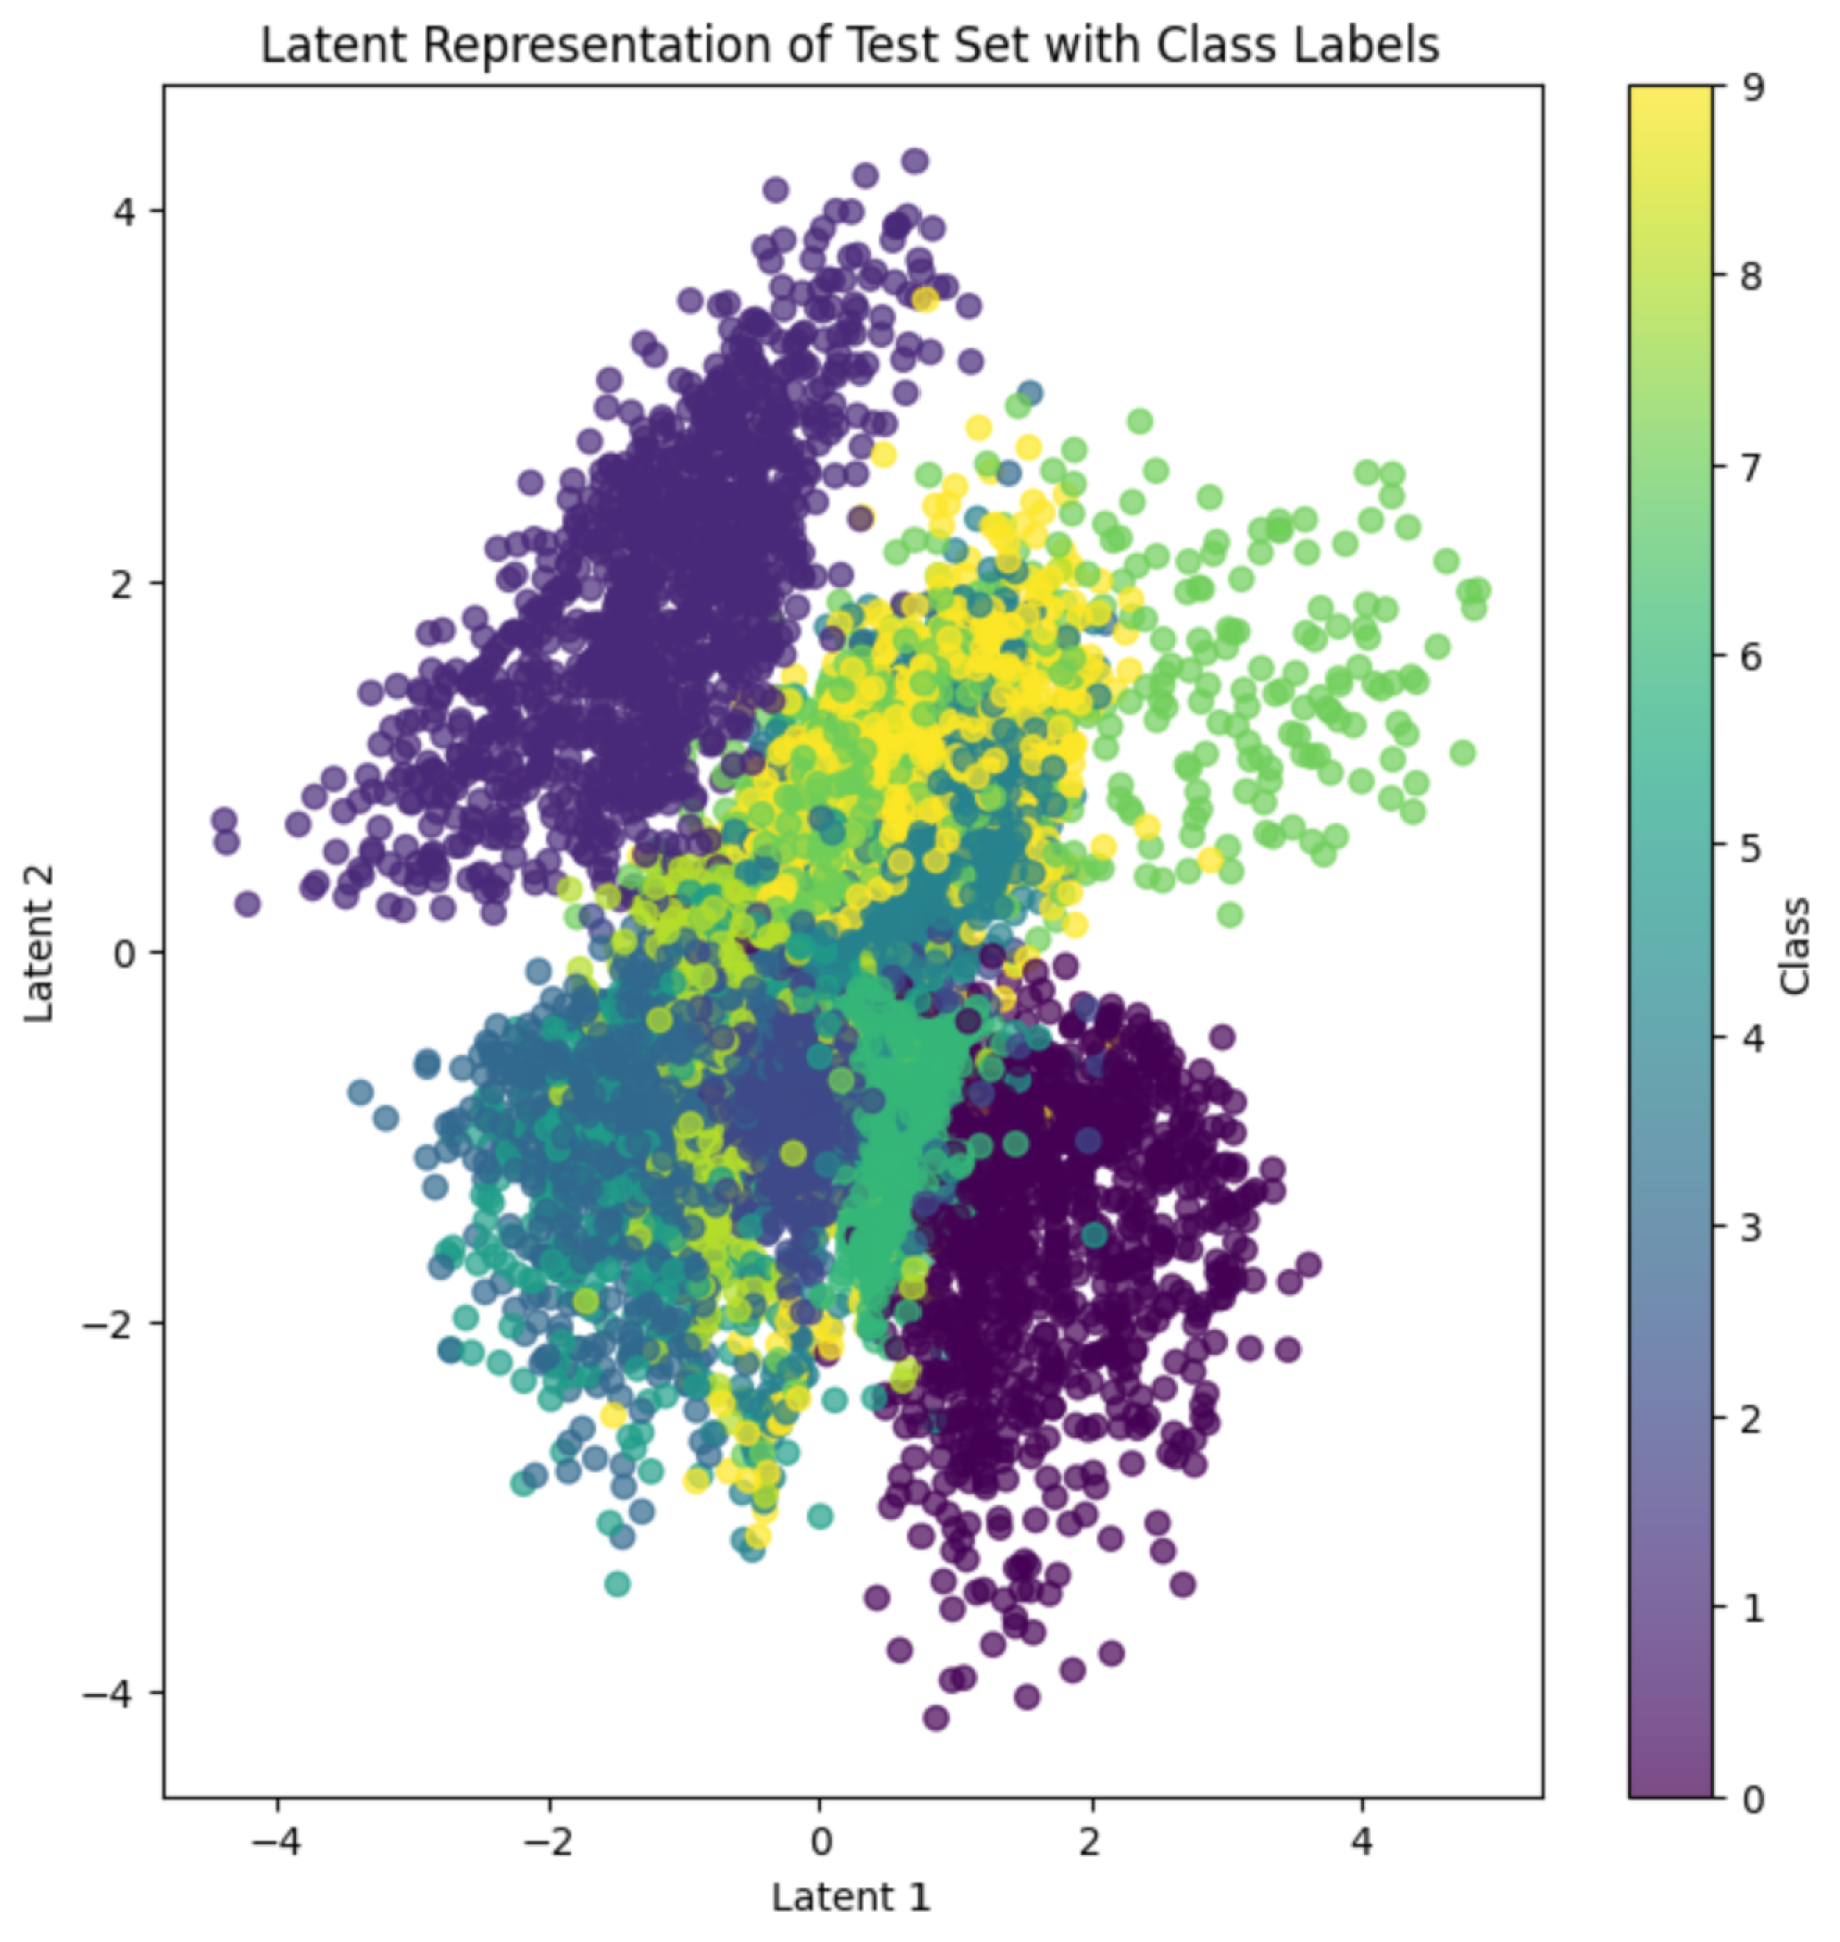
\includegraphics[width=\textwidth]{images/3-latentRep5.png}
        \caption{5 epochs}
        \label{fig:latentRep5}
    \end{subfigure}
    \begin{subfigure}[b]{0.45\textwidth}
        \centering
        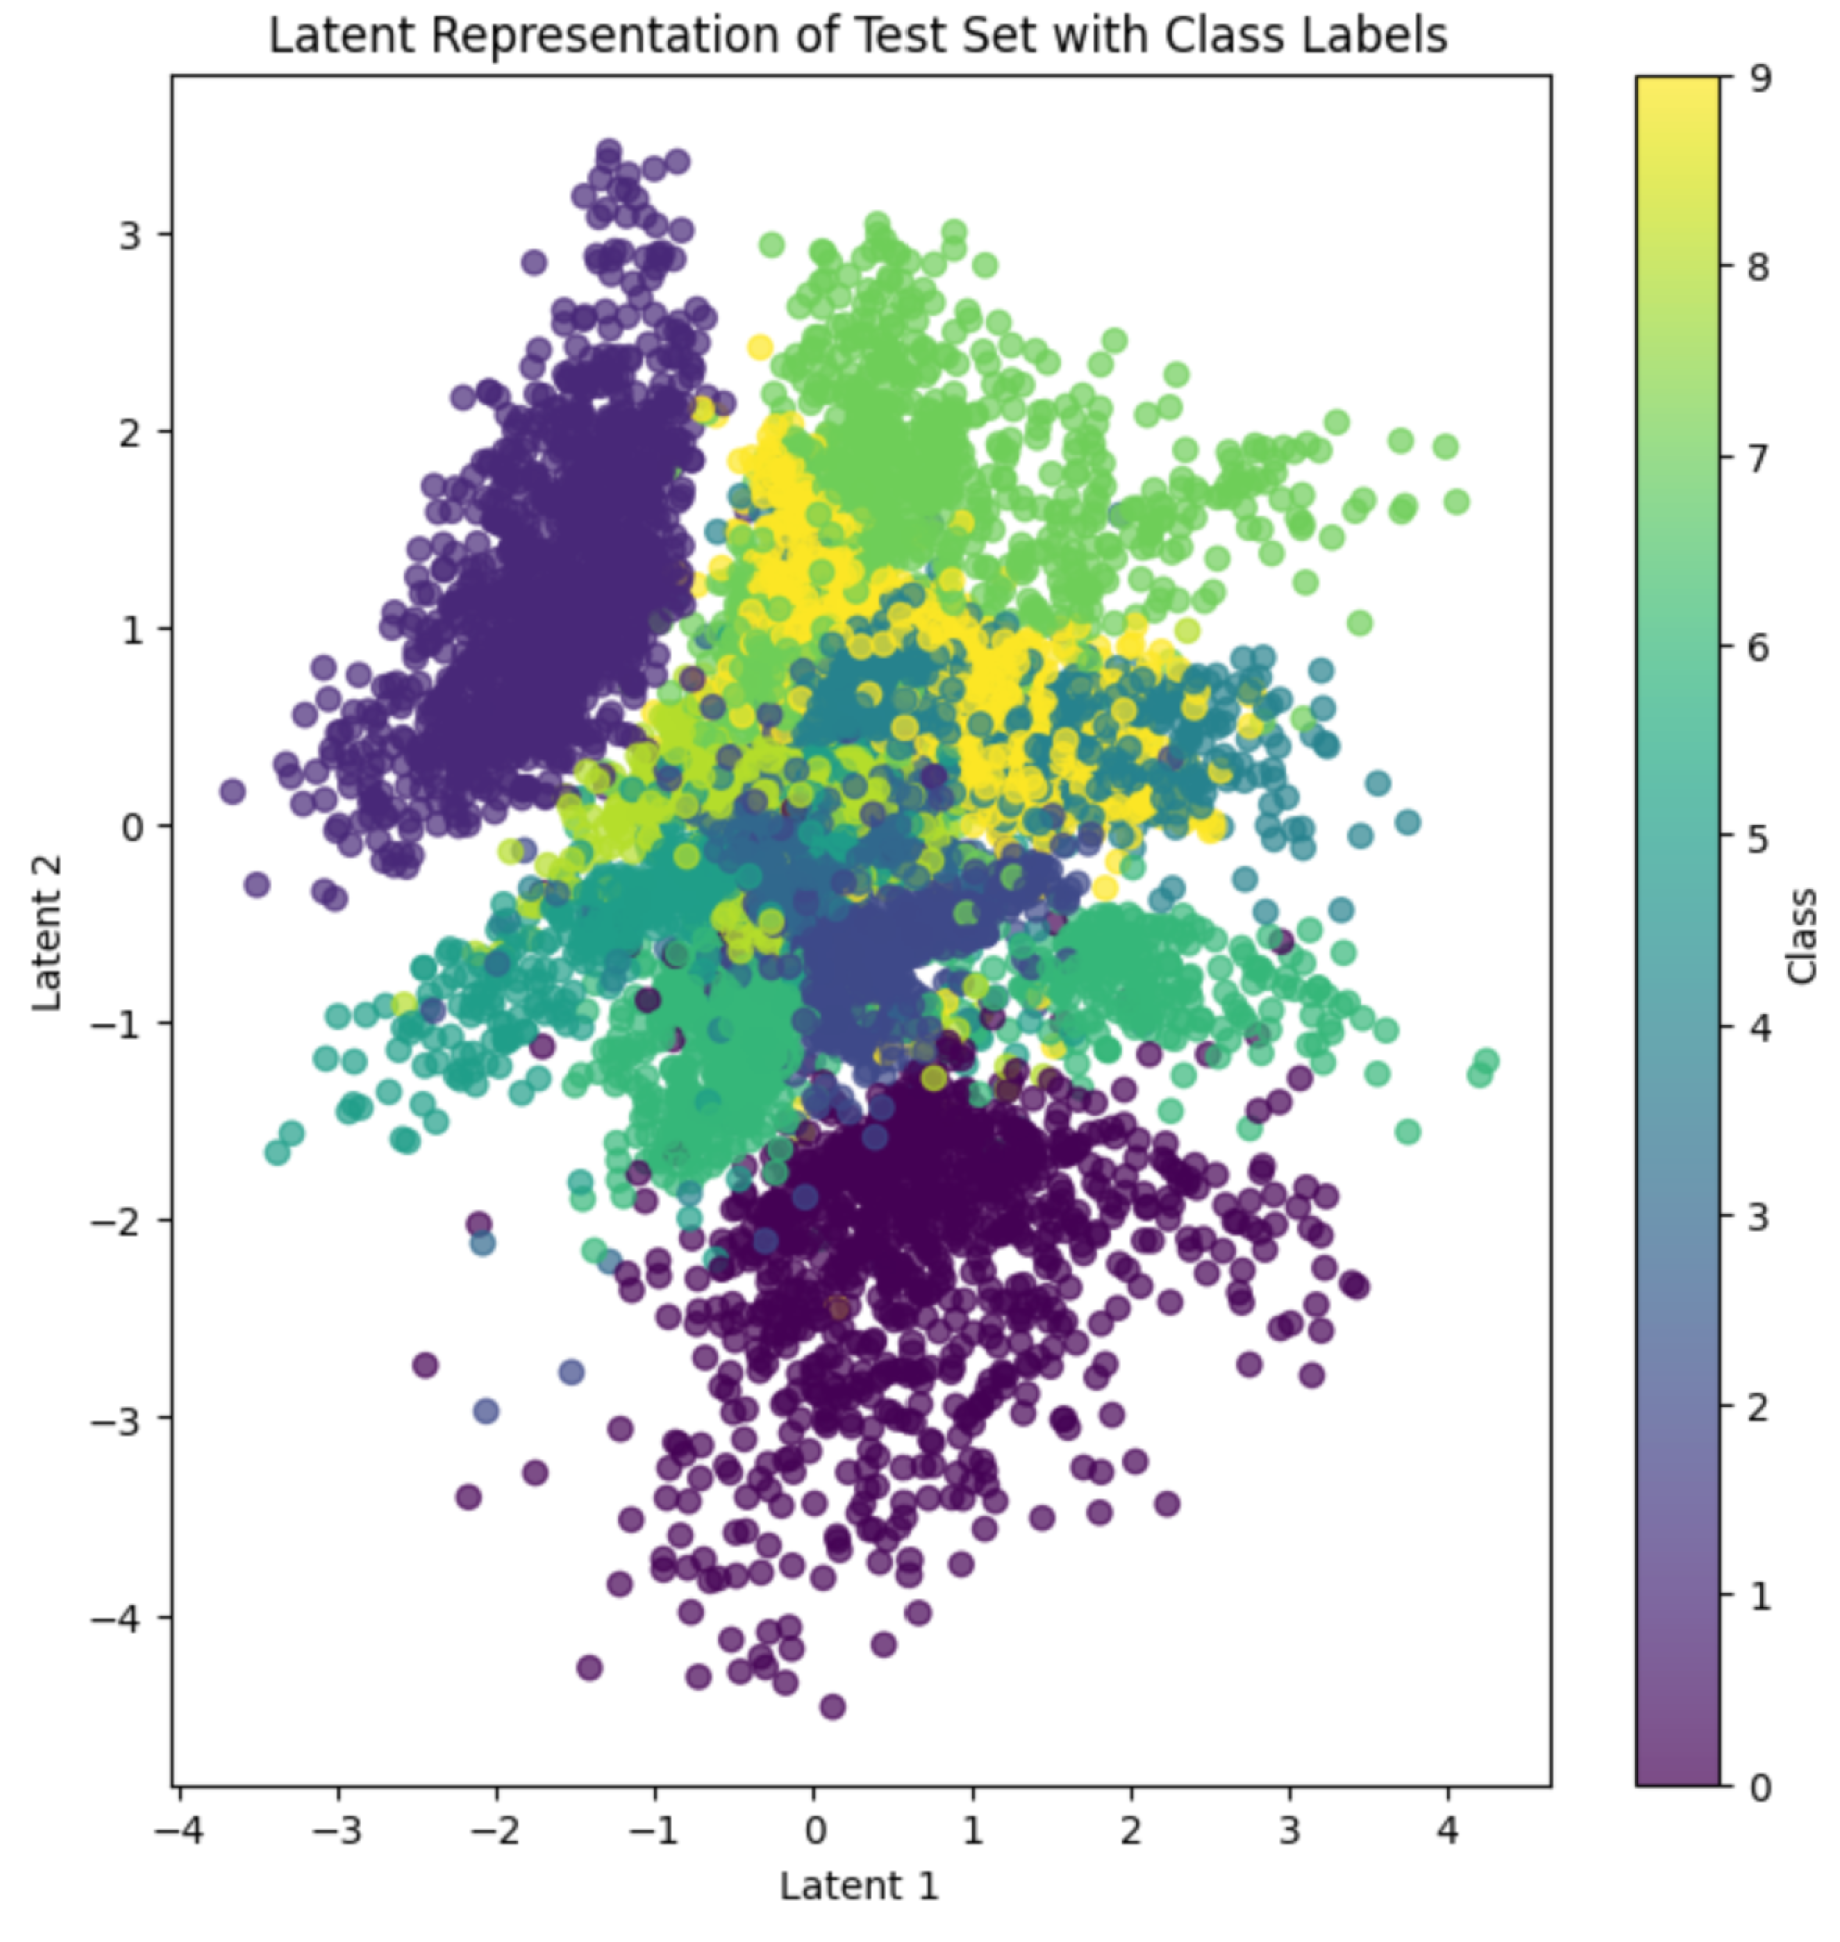
\includegraphics[width=\textwidth]{images/3-latentRep25.png}
        \caption{25 epochs}
        \label{fig:latentRep25}
    \end{subfigure}
    \begin{subfigure}[b]{0.45\textwidth}
        \centering
        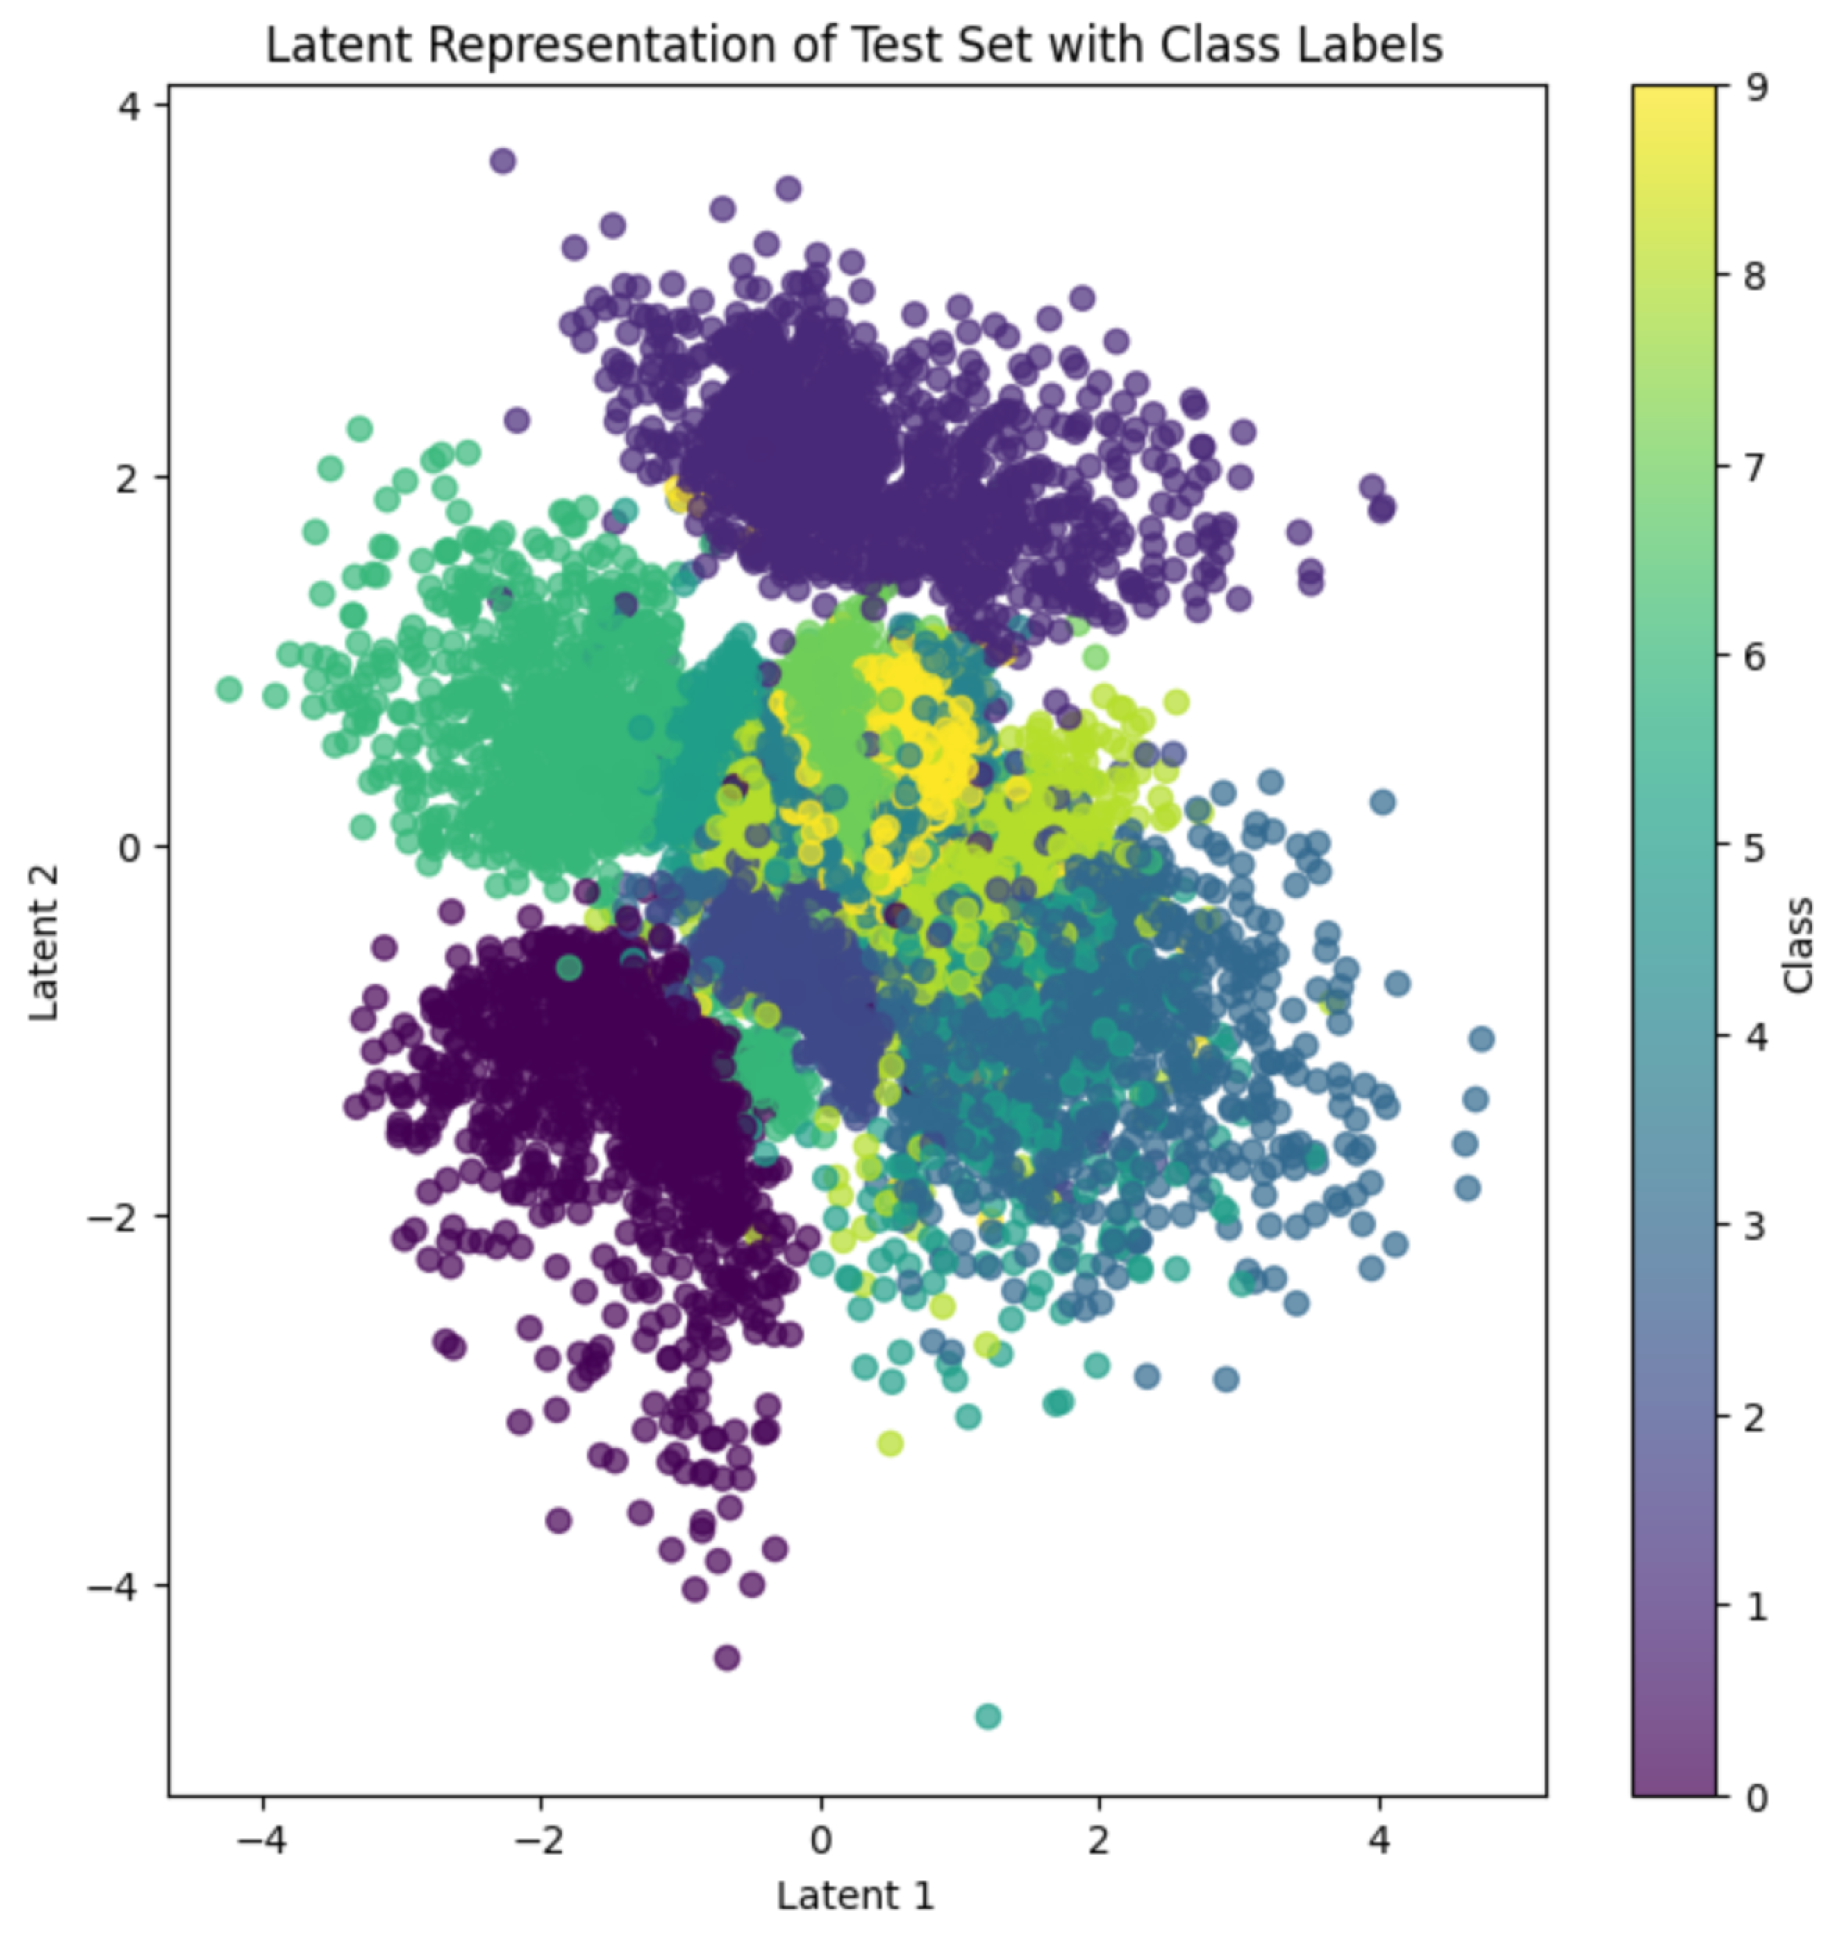
\includegraphics[width=\textwidth]{images/3-latentRep50.png}
        \caption{50 epochs}
        \label{fig:latentRep50}
    \end{subfigure}
    % latent representation after optimisation converged
    \caption{Latent Representation after different numbers of epochs}
    \label{fig:latentRep}
\end{figure}

\begin{figure}[H]\ContinuedFloat
    \centering
    \begin{subfigure}[b]{0.45\textwidth}
        \centering
        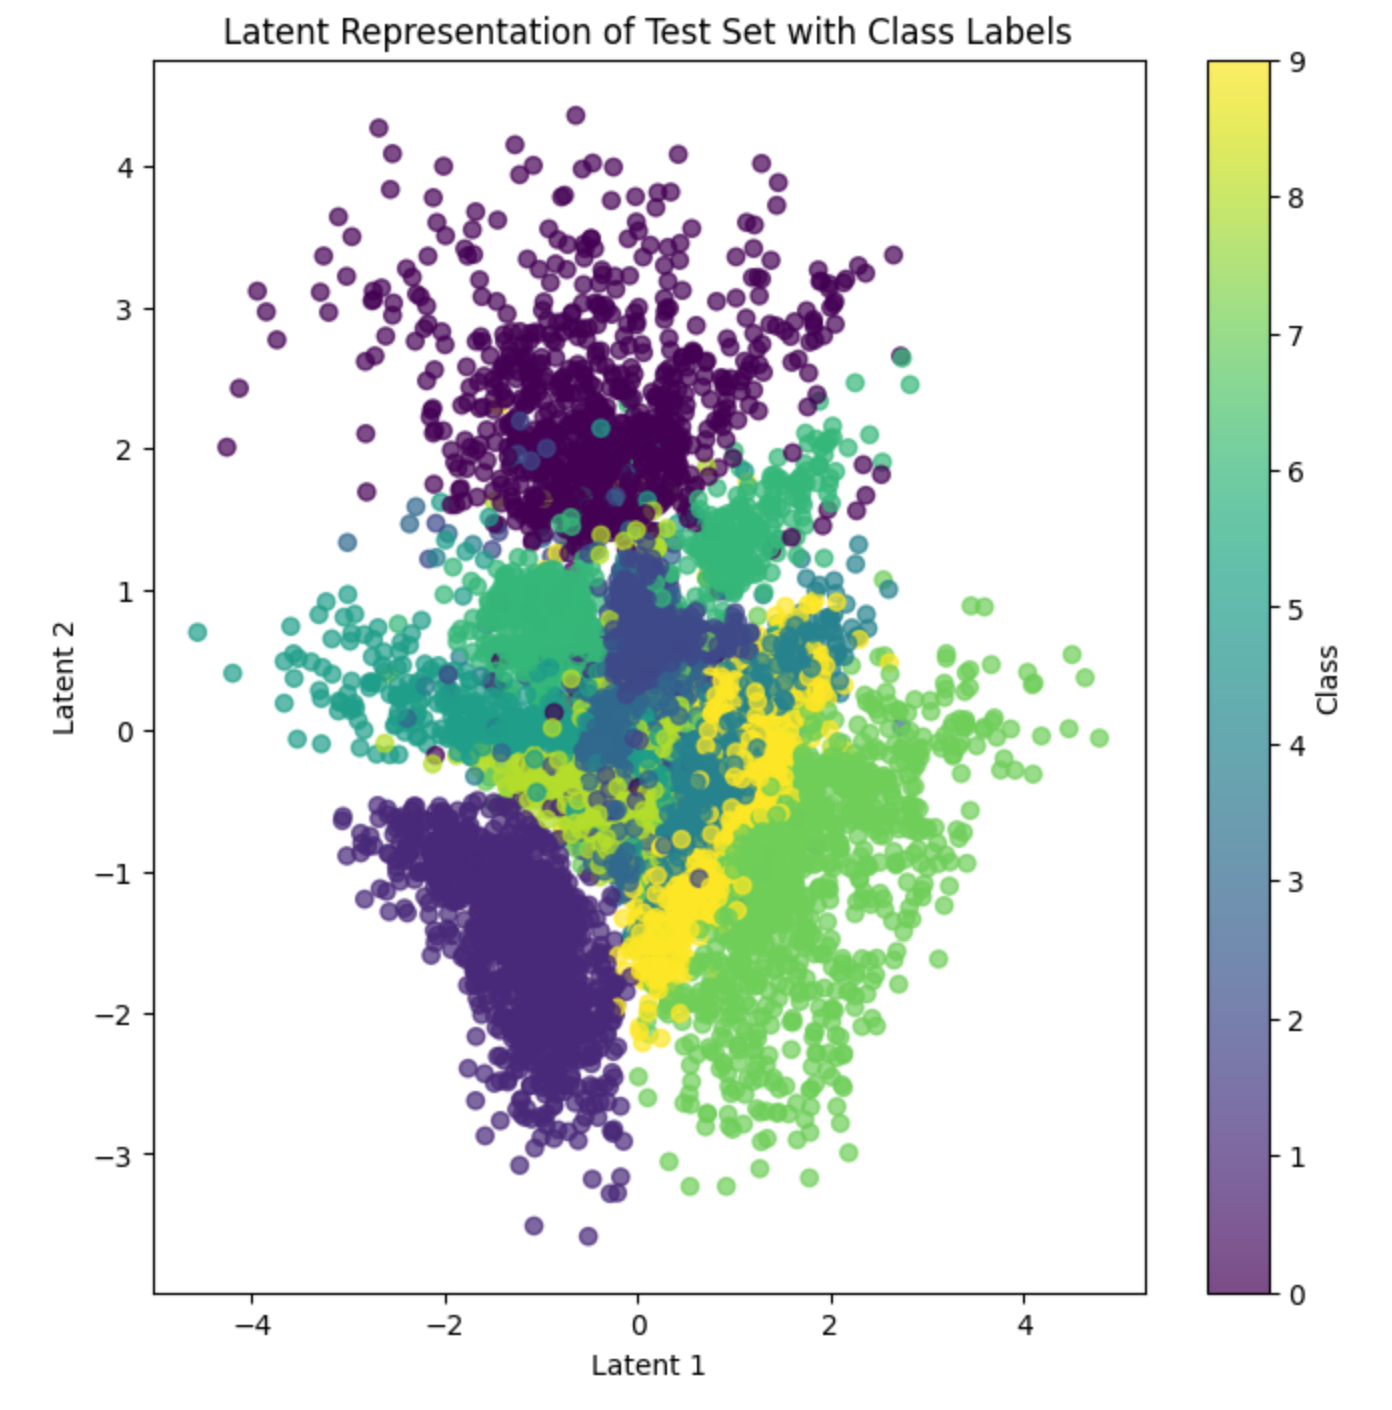
\includegraphics[width=\textwidth]{images/3-latentRepCon.png}
        \caption{after convergence}
        \label{fig:latentRepCon}
    \end{subfigure}
    \caption{Latent Representation after different numbers of epochs}
    \label{fig:latentRep2}
\end{figure}

\textbf{3.2. Plot 15 reconstructed digits and the corresponding original ones.} \\

To generate the reconstructed digits, we use \texttt{$vae.predict(x\_test)$}. Plotting them creates figure \ref{fig:reconstructed}, the subfigures show different training times. After only 1 (\ref{fig:reconstructed1}) and 5 (\ref{fig:reconstructed5}) epochs, it is difficult to achieve proper results for all digits. Increasing the training time to 25 (\ref{fig:reconstructed25}) or 50 (\ref{fig:reconstructed50}) epochs helps to recognize most of the digits and only shows a small difference between both training times. 

Overall, the model works well and 12 of the reconstructed digits depict the correct number for 25 and 50 epochs. Two out of the three errors result from the same digits: A 4 turns into a 9. This mistake is easy to retrace. The two lines on top of the 4 just need to be connected with a slight arc to change the number accordingly. The third error recreates a 4 for 25 epochs, even though the original digit was a 5. This mistake seems unnecessary since multiple lines do not align. For 50 epochs the same digit is problematic and shows a 0. An explanation for the mistakes on this digit is the sloppy handwriting which is distinctly different to a properly written 5. After convergence, even this digit is correctly displayed in the reconstruction. All of the reconstructed digits display a blurriness to them which is to be expected. However, there are methods to reduce blurriness, which again include a larger latent space. \\ 

\begin{figure}[H]
    \centering
    \begin{subfigure}[b]{\textwidth}
        \centering
        
\includegraphics[width=\textwidth]{images/3-originalR.png}
        \caption{Original digits}
        \label{fig:originalR}
    \end{subfigure}
    \begin{subfigure}[b]{\textwidth}
        \centering
        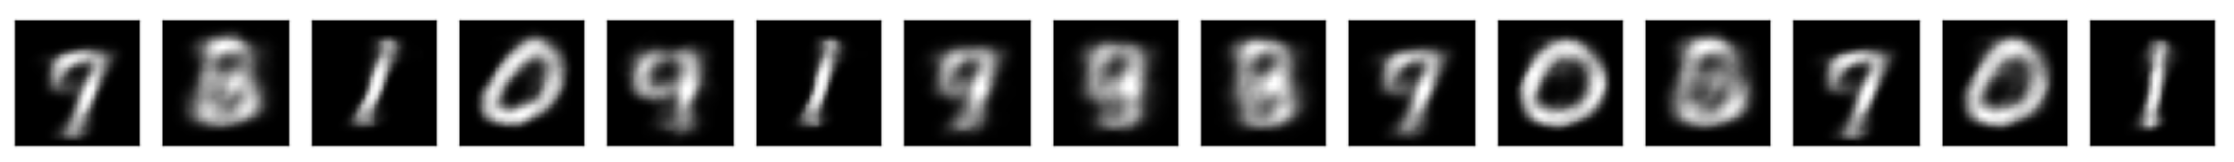
\includegraphics[width=\textwidth]{images/3-reconstructed1.png}
        \caption{1 epoch}
        \label{fig:reconstructed1}
    \end{subfigure}
    \begin{subfigure}[b]{\textwidth}
        \centering
        
\includegraphics[width=\textwidth]{images/3-reconstructed5.png}
        \caption{5 epochs}
        \label{fig:reconstructed5}
    \end{subfigure}
    \begin{subfigure}[b]{\textwidth}
        \centering
        
\includegraphics[width=\textwidth]{images/3-reconstructed25.png}
        \caption{25 epochs}
        \label{fig:reconstructed25}
    \end{subfigure}
    \begin{subfigure}[b]{\textwidth}
        \centering
        
\includegraphics[width=\textwidth]{images/3-reconstructed50.png}
        \caption{50 epochs}
        \label{fig:reconstructed50}
    \end{subfigure}
    \begin{subfigure}[b]{\textwidth}
        \centering
        
\includegraphics[width=\textwidth]{images/3-reconstructedCon.png}
        \caption{after convergence}
        \label{fig:reconstructedCon}
    \end{subfigure}
    \caption{Reconstructed digits after different numbers of epochs}
    \label{fig:reconstructed}
\end{figure}

\textbf{3.3. Plot 15 generated digits, i.e., decode 15 samples from the prior.} \\

To generate new digits, we use \texttt{$decoder.predict(random\_samples)$}. Plotting them creates figure \ref{fig:generated}, the subfigures show different training times. After 1 epoch (\ref{fig:generated1}), barely any digits can be recognized. This changes for 5 (\ref{fig:generated5}) and 25 epochs (\ref{fig:generated25}).  For 50 epochs (\ref{fig:generated50}) the identifiability decreases again slightly. 

Most of the generated digits in figure \ref{fig:generated25} can be recognized as a specific number. The first generated digit could be interpreted either as 1 or as 7. Since the original images showing the number 1 however only consist of a line, the first generated digit most likely corresponds to the number 7. The second digit shows the number 8 with the left side less pigmented making it similar to the number 3. The third digit depicts a problem we already encountered in the reconstructed digits: Numbers 4 and 9 look similar. Both 4 and 9 could be interpreted with a preference towards the number 9. The second digit in the second row is the only image that cannot certainly be assigned a specific number. The remaining digits are easy to recognize and assign. \\

\begin{figure}[H]
    \centering
    \begin{subfigure}[b]{\textwidth}
        \centering
        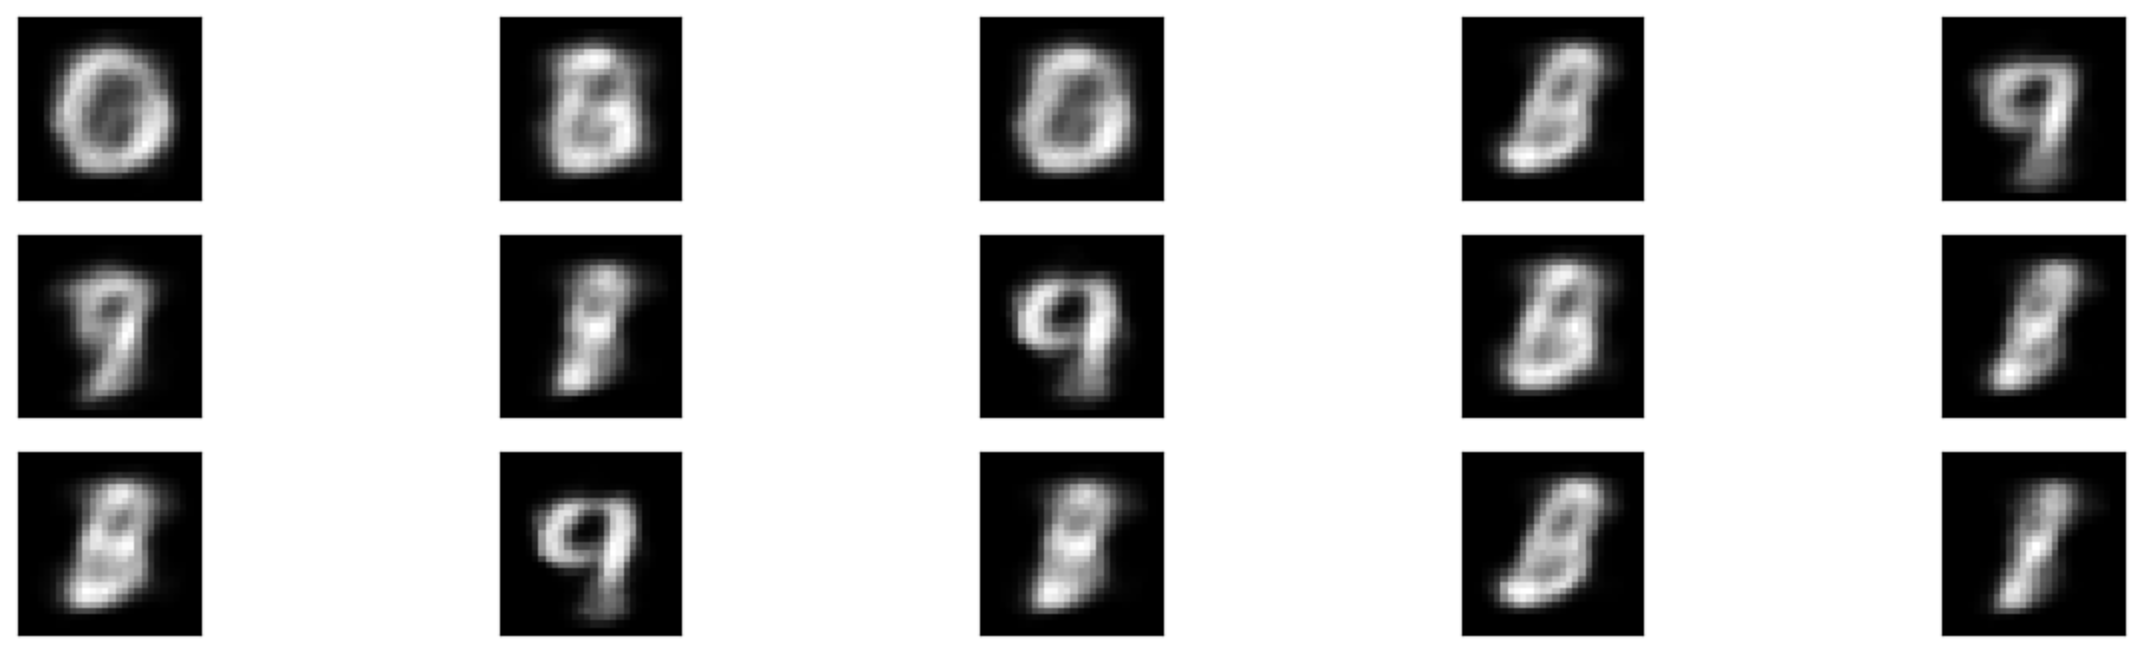
\includegraphics[width=\textwidth]{images/3-generated1.png}
        \caption{1 epoch}
        \label{fig:generated1}
    \end{subfigure}
    \begin{subfigure}[b]{\textwidth}
        \centering
        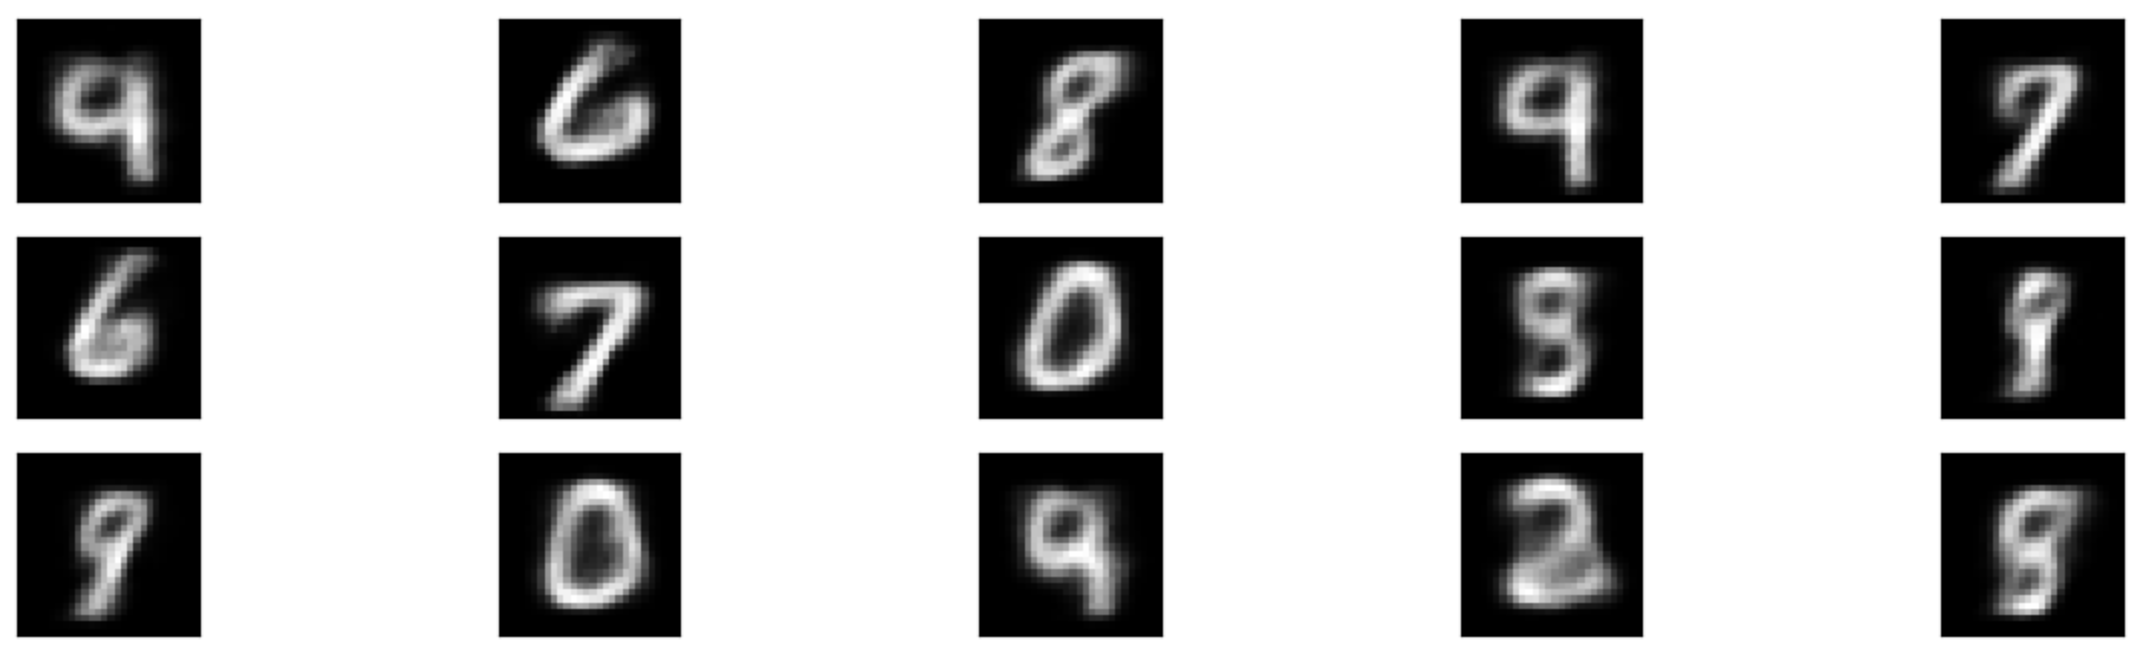
\includegraphics[width=\textwidth]{images/3-generated5.png}
        \caption{5 epochs}
        \label{fig:generated5}
    \end{subfigure}
    \begin{subfigure}[b]{\textwidth}
        \centering
        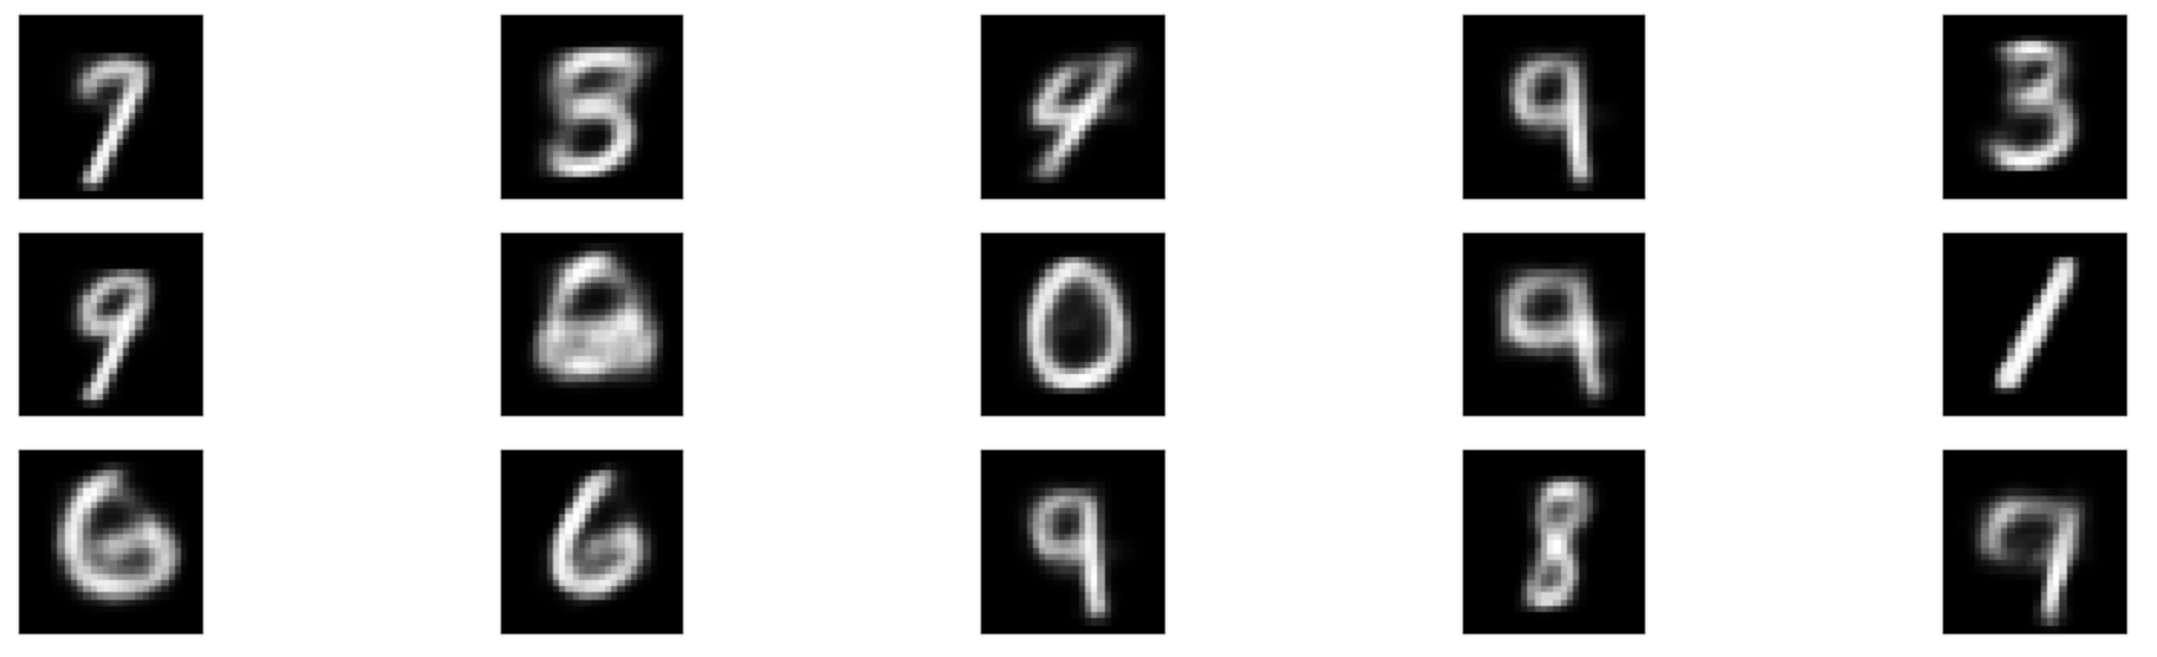
\includegraphics[width=\textwidth]{images/3-generated25.png}
        \caption{25 epochs}
        \label{fig:generated25}
    \end{subfigure}
    \begin{subfigure}[b]{\textwidth}
        \centering
        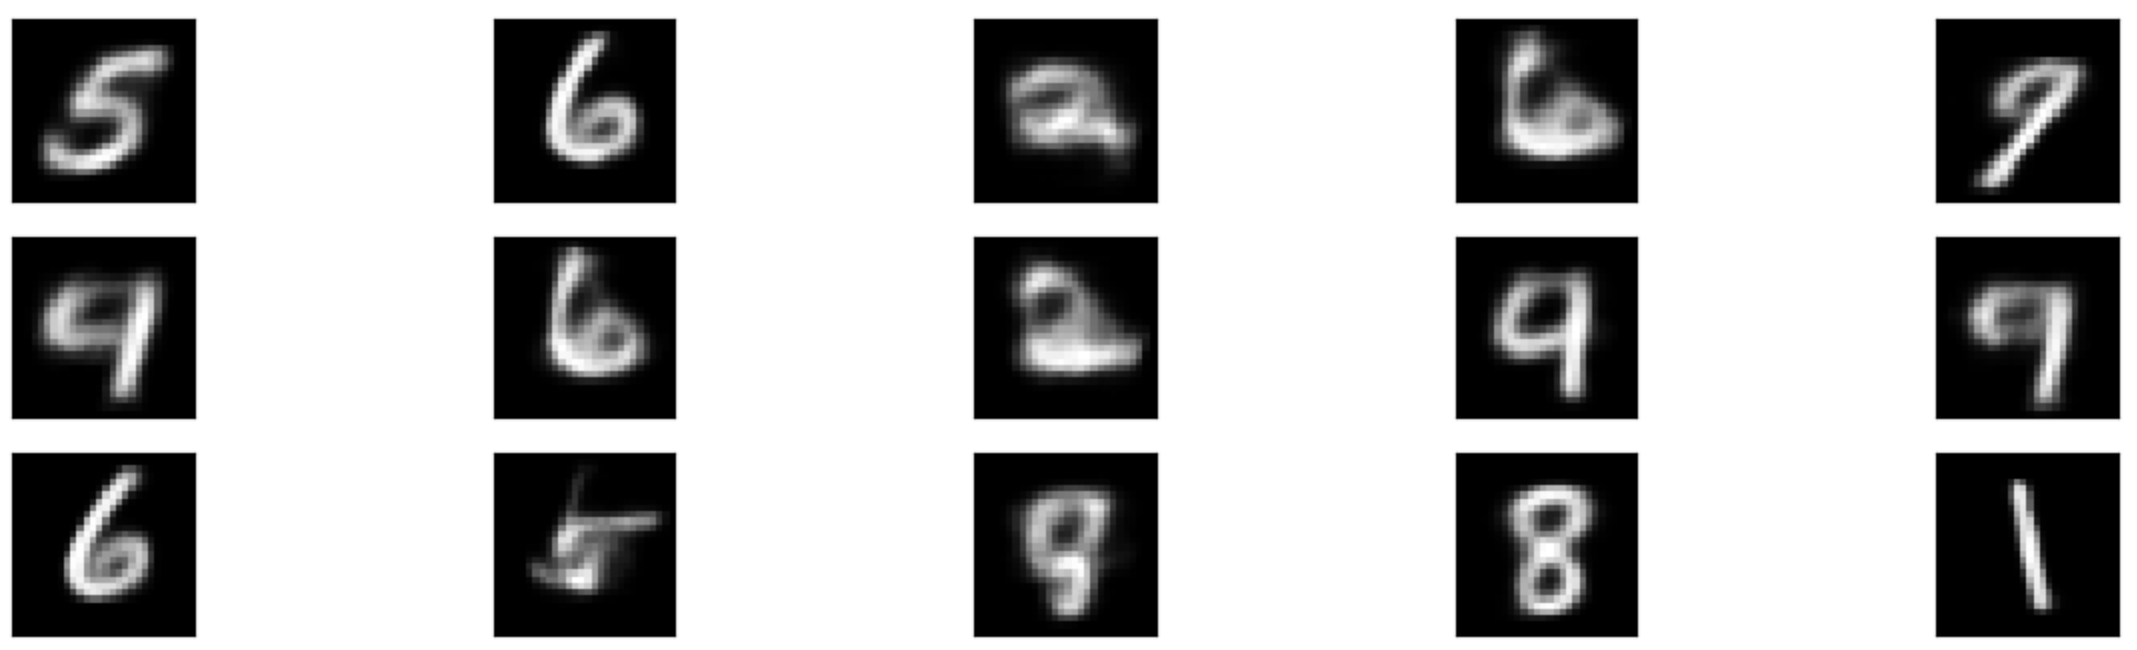
\includegraphics[width=\textwidth]{images/3-generated50.png}
        \caption{50 epochs}
        \label{fig:generated50}
    \end{subfigure}
    % generated after optimisation converged
    \caption{Generated digits after different numbers of epochs}
    \label{fig:generated}
\end{figure}

\begin{figure}[H]\ContinuedFloat
    \centering
    \begin{subfigure}[b]{\textwidth}
        \centering
        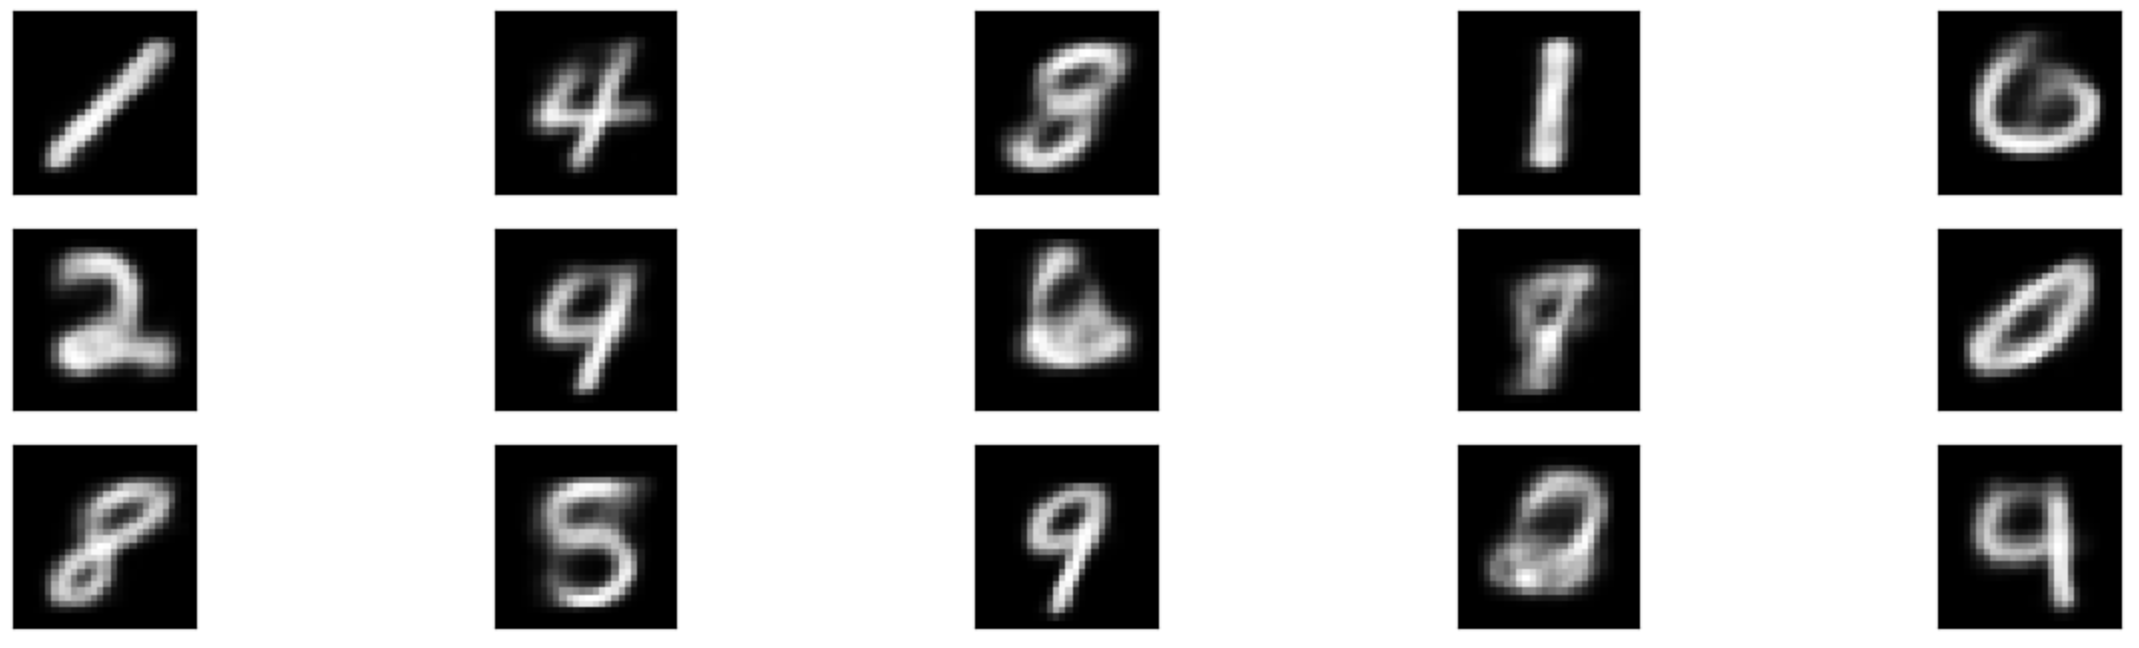
\includegraphics[width=\textwidth]{images/3-generatedCon.png}
        \caption{after convergence}
        \label{fig:generatedCon}
    \end{subfigure}
    \caption{Generated digits after different numbers of epochs}
    \label{fig:generated2}
\end{figure}

\textbf{4. Plot the loss curve} \\

ELBO loss stands for 'evidence lower bound loss' and is commonly used in VAEs. Figure \ref{fig:elbo} shows the loss development over the epochs. In the first two epochs, the training loss drops quickly to a value of $165.5712$, the test loss being slightly lower at $162.4413$. After that, the loss decreases slowly until we achieve a training loss of $141.2879$ and a test loss of $141.8026$. This behavior is what was expected. The values of training and test loss leave a small generalization gap, meaning that our model is able to perform well on unseen data as well. Since the training loss curve is still going down when we stop training, the model is not overfitting and we could possibly increase the training time (amount of epochs) to achieve the best possible outcome given the same parameters. \\ 

\begin{figure}[hbt!]
    \centering
    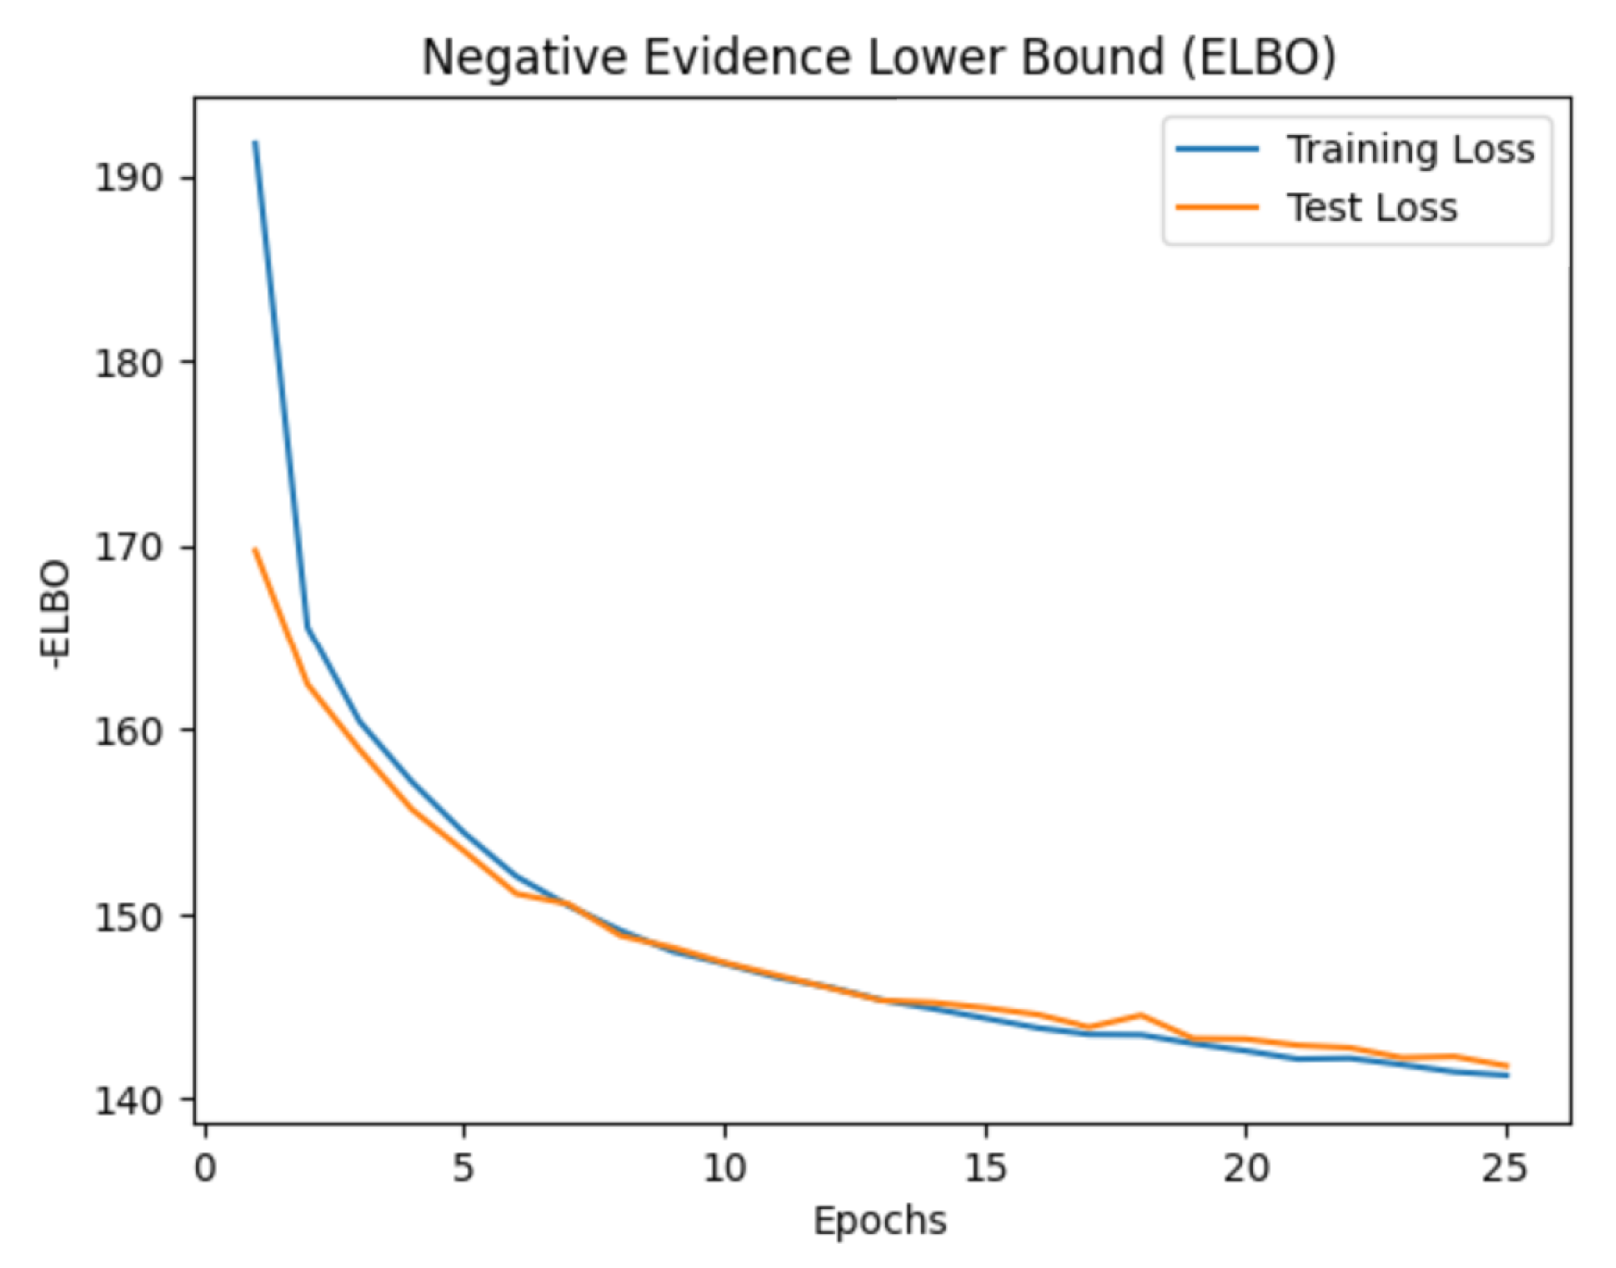
\includegraphics[width=0.7\textwidth]{images/3-ELBO.png}
    \caption{ELBO Loss vs. epochs on 2-dimensional latent space}
    \label{fig:elbo}
\end{figure}

\newpage
\textbf{5. Train the VAE using a 32-dimensional latent space} \\

% 5.1. Compare 15 generated digits with the results in 3.3.
Despite our assumption, increasing the latent space does not generate better digits with a training time of 25 epochs. In figure \ref{fig:generated-32}, the depicted digits are less recognizable, less than half of them can be assigned a certain number. \\


\begin{figure}[H]
    \centering
    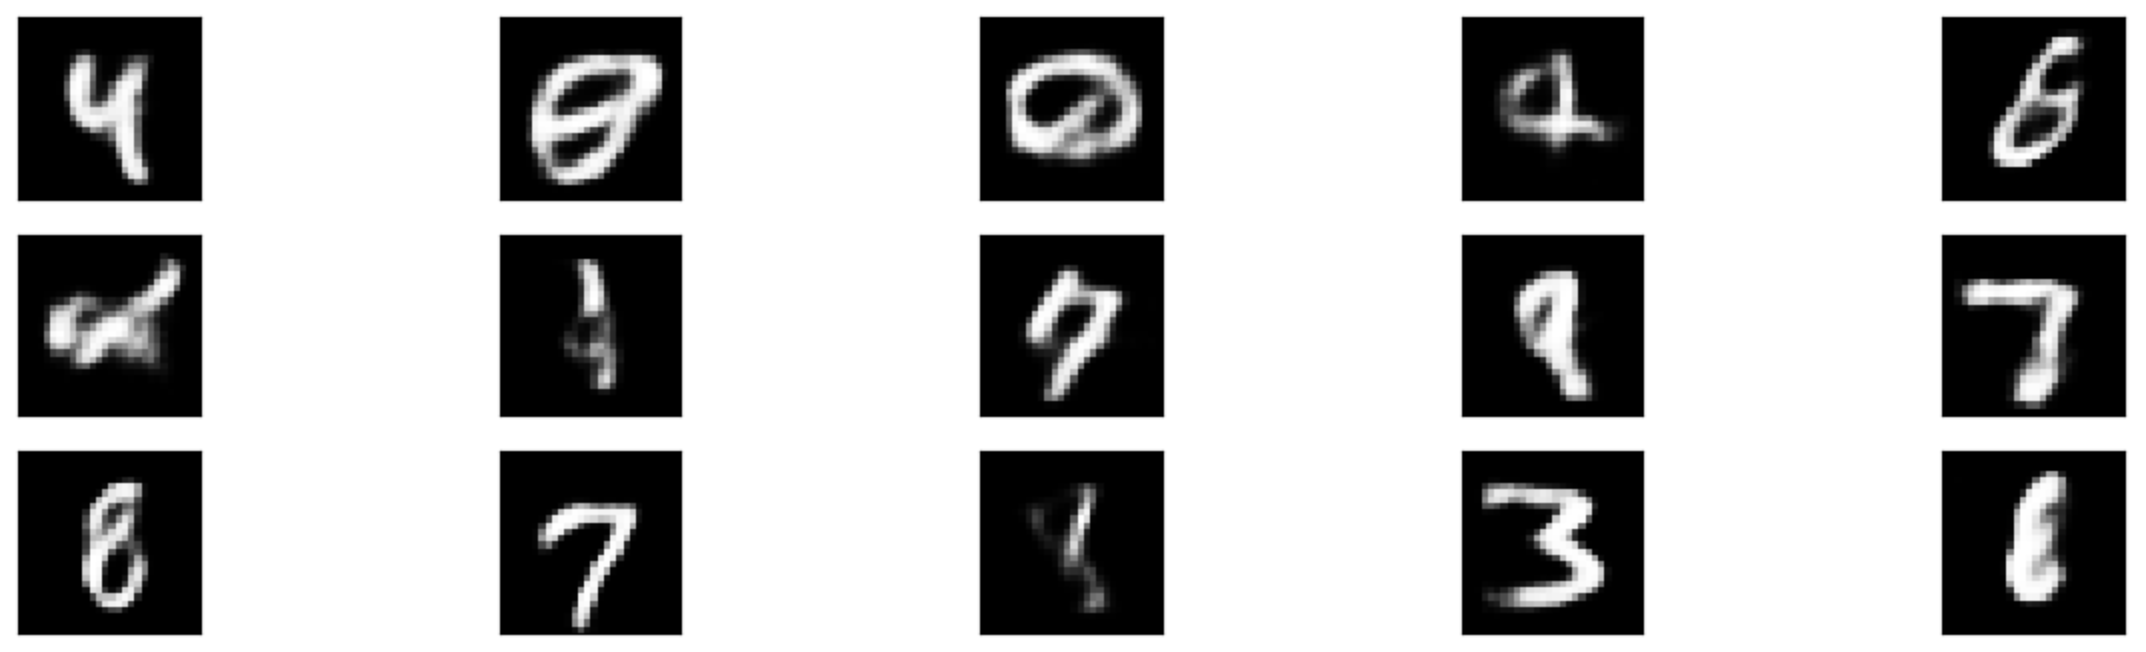
\includegraphics[width=\textwidth]{images/3-generated-32.png}
    \caption{Generated digits on 32-dimensional latent space}
    \label{fig:generated-32}
\end{figure}

% 5.2. Compare the loss curve with the one in 4.
At first glance, figure \ref{fig:elbo32} looks similar to the previously generated loss curve. Once we take a closer look, we notice that increasing the latent space to 32 has a positive effect on the loss: After just two epochs, the loss already dropped to $129.1468$ for the training and $120.9672$ for the test, both values are lower than the previous loss after our full training time. In comparison to the last test loss, it is more stable now and does not depict any spikes in its curve. After the 25th epoch, we reach a training loss of $101.1582$ and a test loss of $101.0482$ which is significantly better with a difference of roughly $40$ each. Again, we can see that the training loss is still decreasing in the end. This time, however, the decrease involves only decimals.  

\begin{figure}[H]
    \centering
    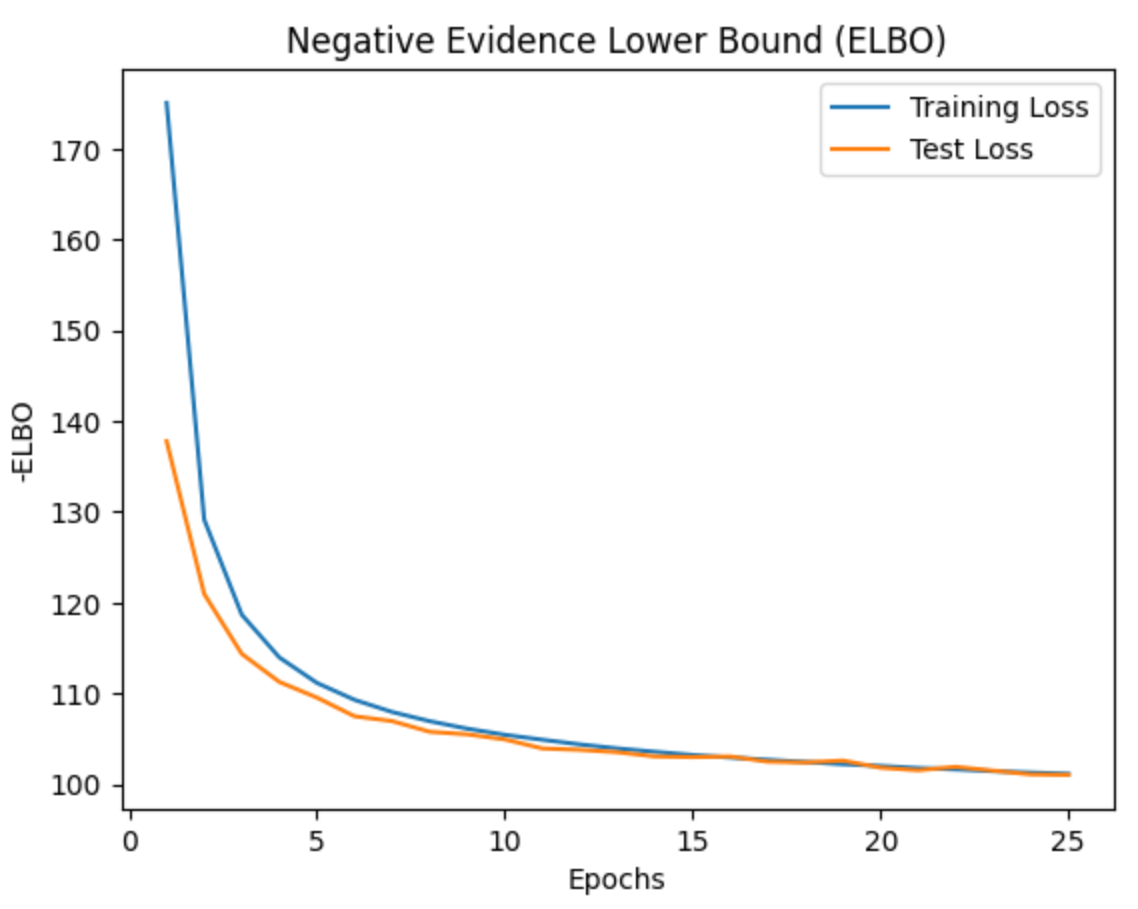
\includegraphics[width=0.7\textwidth]{images/3-ELBO32.png}
    \caption{ELBO Loss vs. epochs on 32-dimensional latent space}
    \label{fig:elbo32}
\end{figure}

% time estimate : 
Approximately 15hours have been needed in order to implement and test the VAE model itself.
% accuracy : 


% what we learned about data and method : 
    % by increasing the dimensionality of the latent space 
The observations made in 5. prove that simply increasing the latent space of a model doesn't necessarily improve its performance and it can be explained by the fact that the model isn't complex enough to deal with the added capacity of representation brought by the larger latent space and/or by the fact that the dataset's complexity (here the MNIST) doesn't warrant a larger latent space as it has a low intrinsic dimensionality itself. 
\end{task}

\newpage
\begin{task}{4, Metrics and Comparison}
% We'll compare the values obtained for different metrics (distances, embedding, Riemannian Metric) to assess quality performance differences between the two packages. Context and different parameters used (in dataset size and dimensions in particular) will also be taken into account to nuance our statements. 

% Distances: Compare how distances between points in the high-dimensional space are preserved in the low-dimensional embeddings.

% Embedding Quality: Evaluate the embeddings visually (if 2D or 3D) and statistically (e.g., using metrics like trustworthiness or continuity).

% Riemannian Metric: If the methods involve calculating a Riemannian metric (which provides a way to measure geometric properties of the data manifold), compare these metrics. This might require advanced mathematical computations.

% -----------------------------

% Megaman: RiemannianMetric: This class produces the estimated Riemannian metric Ri at each
% point i given an embedding y1:N and the estimated Laplacian from the original data.

We considered different metrics to use for comparison of our results to the ones specified in the paper. Since we cannot precisely recreate the same level of accuracy, comparing the runtime to the one in the paper is not an option. Instead, we took a look at the Riemannian metric as well as trustworthiness. \\

\textbf{Riemannian metric} \\
"A Riemannian metric g is a symmetric and positive definite tensor field which defines an inner product $<,>_g$ on the tangent space $T_p\M$ for every $p \in \M$." \cite{perrauljoncas2013nonlinear}

It is used to define distances and angles on a smooth manifold, which is a generalization of surfaces to higher dimensions. Mathematically, a Riemannian metric on a manifold M is often denoted by a positive definite symmetric bilinear form g, defined on the tangent space at each point:\\

$g_p : T_pM \times T_pM \rightarrow \R$ \\

Here, $T_pM$ is the tangent space at a point $p$ on the manifold, and $g_p$ is the Riemannian metric at that point. 
The Riemannian metric allows for the calculation of lengths of curves, angles between curves, and various other geometric properties of the manifold. \\

We ultimately decided to use trustworthiness which is an easy concept to grasp. Additionally, it has the advantage that we can use one metric for all algorithms used in our project. \\

\textbf{Trustworthiness} \cite{trust-sk} \\
Trustworthiness is a score that displays to what extent the local structure is maintained. It is always a floating point number within [0, 1] and can be computed as follows: 
\begin{equation}
    T(k) = 1 - \frac{2}{nk(2n-3k-1)} \sum_{i=1}^{n} \sum_{j \in \N_i^k} max(0, (r(i,j)-k))
\end{equation}

For each sample i, its k nearest neighbors in the output space are denoted as $\N_i^k$,
and every sample j is its $r(i,j)$-th nearest neighbor in the input space. This means that any unanticipated nearest neighbors in the output space are penalised in proportion to their rank in the input space. \\

This metric needs to calculate the distance matrix for each point in the dataset which becomes a problem as our memory is not big enough to store this calculated matrix. In order to get a general idea of trustworthiness, we employed mini batching. We picked a subset of 10,000 vectors and calculated the trustworthiness of this smaller subset and finally calculated the mean of all of the subsets to find an approximate trustworthiness metric. This approach may not be very suitable as we need to look at the entire dataset to calculate our metric, but it gives us an approximate value to compare. \\

\textbf{Timings}\\
We can also compare the runtime between different libraries by utilizing one standard computer and recording the runtime. Although this is not a very good way of comparing the libraries and the neural network, it can provide us with an insight into the libraries' performances. We used Google Colab which provides us with 12.7 GB of memory to run our code and record the runtime for calculation of embeddings.\\


\textbf{Comparisons}\\
We show comparison values only for the \textit{Swiss Roll Curve} dataset. We decided not to include the Word2Vec dataset as the results were unsatisfactory.
\begin{itemize}
    \item \textbf{Trustworthiness}\\
    Table \ref{tab:library-comparison} shows the different values of trustworthiness scores obtained by different libraries and approaches. The empty cells for 1M points show that the libraries were unable to run on the big datasets. Generally, an improvement from using 10k points can be recognized when using 100k points instead. The best trustworthiness scores for 100k and 1M points are highlighted in their corresponding columns. 
    \begin{table}[h]
    \centering
    \begin{tabular}{|l|c|c|c|}
        \hline
        \textbf{Library Name} & \textbf{10k Points} & \textbf{100k Points} & \textbf{1M Points} \\
        \hline
        \hline
        Sklearn & 0.5001 & 0.9916 & - \\
        \hline
        Datafold & 0.9993 & 0.9992 & - \\
        \hline
        Datafold (Roseland) & 0.9993 & \textbf{0.9993} & 0.9989 \\
        \hline
        UMAP & \textbf{0.9998} & 0.9801 & - \\
        \hline
        Autoencoder & 0.9994 & 0.9986 & \textbf{0.9991} \\
        \hline
    \end{tabular}
    \caption{Comparison of Libraries on Different Datasets}
    \label{tab:library-comparison}
\end{table}
    \item \textbf{Timings}\\
    Table \ref{tab:library-comparison-timings} shows the timings taken by different libraries to calculate the embeddings. We do not include UMAP here, as it uses GPU and would not be a fair comparison. Again, the empty cells for 1M represent that the library was not able to calculate the embeddings of the dataset. While Sklearn is by far the fastest library for 100k points, Datafold (Roseland) ranks second with less than one minute. Considering it also provides the best trustworthiness score, it can be seen as a winner on 100k points. For 1M points, however, Autoencoder performs better for both trustworthiness and computation time. \\
    \begin{table}[h]
    \centering
    \begin{tabular}{|l|c|c|c|}
        \hline
        \textbf{Library Name} & \textbf{10k Points} & \textbf{100k Points} & \textbf{1M Points} \\
        \hline
        \hline
        Sklearn & \textbf{1.3} & \textbf{10.0} & - \\
        \hline
        Datafold & 6.2 & 485.1 & - \\
        \hline
        Datafold (Roseland) & 6.9 & 51.3 & 4357.8 \\
        \hline      
        Autoencoder & 68.5 & 142 & \textbf{1282.7} \\
        \hline
    \end{tabular}
    \caption{Time comparison of Libraries on Different Datasets(in seconds)}
    \label{tab:library-comparison-timings}
    \end{table}
    \textit{Note: }The timings for Autoencoder is the training time for 50 epochs. 
\end{itemize}


% cuML also provides this metric within \texttt{cuml.metrics.trustworthiness} \cite{trust-cuml}, it can be called with the parameters listed below: 
% \begin{itemize}
%     \item X: array-like, shape = (n\_samples, n\_features) \\
%     The original data
%     \item X\_embedded: array-like, shape = (n\_samples, n\_features) \\
%     The compromised low-dimensional data
%     \item n\_neighbors: int, optional (default=5) \\
%     Number of neighbors considered
%     \item metric: str in ['euclidean'] (default='euclidean') \\
%     Metric used to compute the trustworthiness. For the moment only ‘euclidean’ is supported
%     \item convert\_dtype: bool, optional (default=False) \\
%     When set to True, the trustworthiness method will automatically convert the inputs to np.float32
%     \item batch\_size: int (default=512) \\
%     The number of samples to use for each batch.
% \end{itemize}
% The \texttt{trustworthiness} function returns a double score. We specified X as well as X\_embedded and kept the other parameters as their default values. \\

% With cuML's \texttt{trustworthiness}, we achieved the following results: 
\end{task}

\begin{task}{5, Conclusion and future work}
% - add recovered state
% - add probability to become recovered
In order for us to add the recovered class and visualize them properly, we had to change the following files:
\begin{itemize}
    \item \textbf{AttributesSIRG:} 
    \begin{itemize}
        \item New method \texttt{getRecoveredfixedRate()} which returns the new value of \texttt{recoveredfixedRate} set arbitrarily at 0.2 (the probability for an INFECTED individual to become recovered/removed).
    \end{itemize}

    \item \textbf{SIRType:} 
    \begin{itemize}
        \item Added the type \texttt{ID\_REMOVED} for the removed group.
    \end{itemize}

    \item \textbf{SIRGroupModel:} 
    \begin{itemize}
        \item To include the removed class, we had to change the method \texttt{getFreeGroupId()} to include the new group of recovered individuals. Figure \ref{fig:SIRGroupModel_code_change} shows the change in the function. It was a simple fix to include the recovered class with a similar logic as the infected group. We also had to change the \texttt{Update function} to add infected individuals to the recovered class based on a certain probability. 
        \begin{figure}[h]
            \centering
            \begin{subfigure}[b]{0.5\textwidth}
                 \centering
                 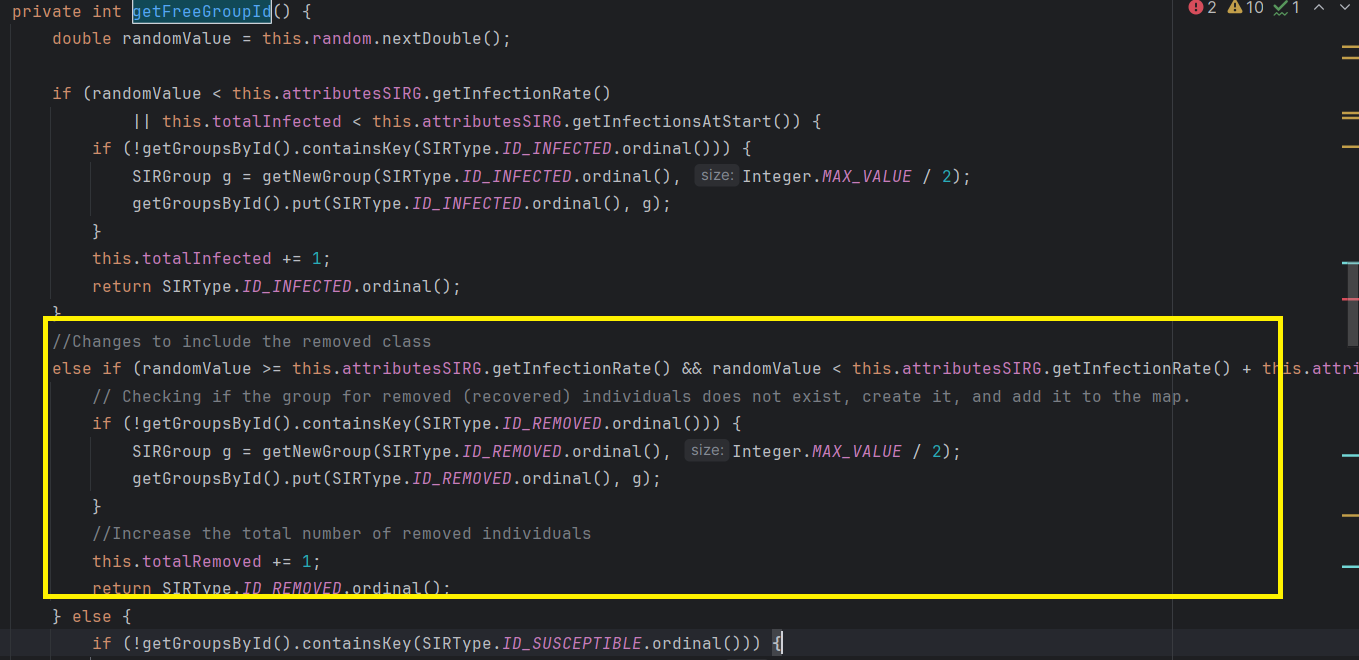
\includegraphics[width=\textwidth]{images/removedClassCode.png}
                \caption{getFreeGroupId() changes in SIRGroupModel}
                \label{task5CodeChangea}
             \end{subfigure}
            \begin{subfigure}[b]{0.5\textwidth}
                 \centering
                 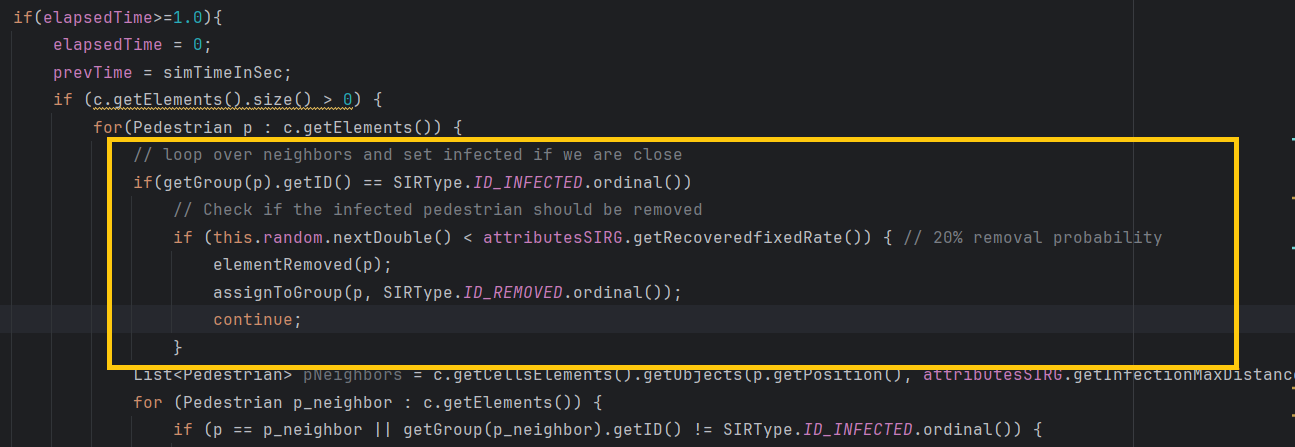
\includegraphics[width=\textwidth]{images/removedClassCOdeChange2.png}
                \caption{Changes in update method of SIRGroupModel}
                \label{fig: task5CodeChangeb}
             \end{subfigure}
            \caption{Code changes in SIRGroupModel to include recovered class.}
            \label{fig:SIRGroupModel_code_change}
        \end{figure}
    \end{itemize}

    \item \textbf{utils.py:} 
    \begin{itemize}
        \item We changed the function \texttt{create\_folder\_data\_scatter(folder)} in the provided SIRVisualization utils file (\texttt{DASH/plotly} visualizer) to allow us to visualize the recovered class.
    \end{itemize}
\end{itemize}




% - visualisation
% - tests

To test our implementation we conducted multiple experiments on our modified software. The first test we conduct is the same as in figure \ref{fig:task4.5_1} from task 4, with the only difference that pedestrians now can recover after being infected. The end frame for task 5 can therefore look like the ones in figure \ref{fig: 51ad}, with different distributions of blue and green dots for susceptible and recovered pedestrians. \\
Figure \ref{fig: 5ad} shows a comparison of different infection and recovery rates. In subfigure \ref{fig: 5a}, a low infection rate (0.05) and a high recovery rate (0.2) are used. Only 202 pedestrians become infected over time and a constant value is established after 70 time steps. In subfigure \ref{fig: 5b}, the infection rate is doubled (0.1), while the recovery rate stays the same (0.2). In comparison, a drastic difference can be seen: the susceptible and removed lines almost close the gap in between with a total number of 473 infected and later removed pedestrians after 60 time steps. Subfigure \ref{fig: 5c} changes the recovery parameter to 0.1, and the infection parameter stays at 0.1. Here, the initial spike in infections is much higher, and a total of 790 infections after 86 time steps. Finally, subfigure \ref{fig: 5d} is created with an infection rate of 0.05 and a recovery rate of 0.1. It looks the closest to the second parameter settings, however, the lines intersect, and the infections reach a total of 630 after 103 time steps.

\begin{figure}[H]
 \centering
 \begin{subfigure}[b]{0.4\textwidth}
     \centering
     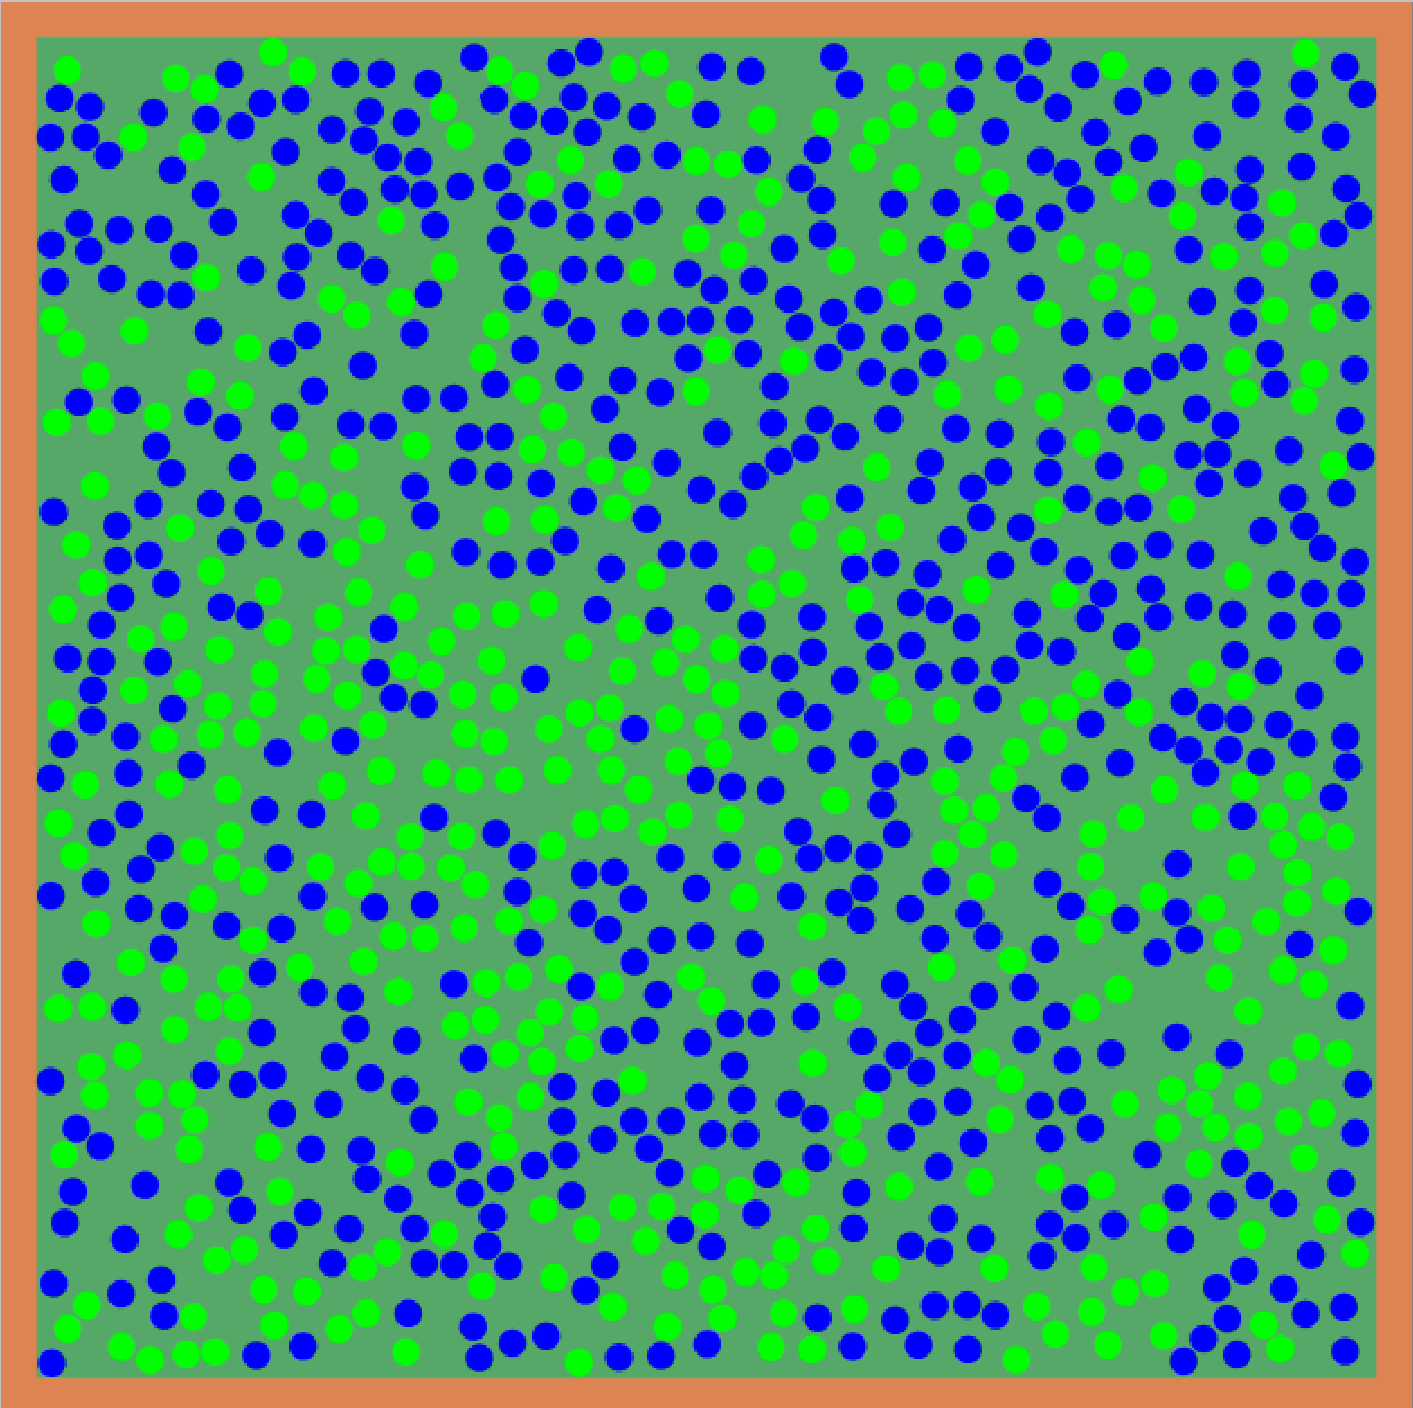
\includegraphics[width=0.8\textwidth]{images/2-51a.png}
    \caption{I: 0.05 - R: 0.2}
    \label{fig: 51a}
 \end{subfigure}
 \begin{subfigure}[b]{0.4\textwidth}
      \centering
     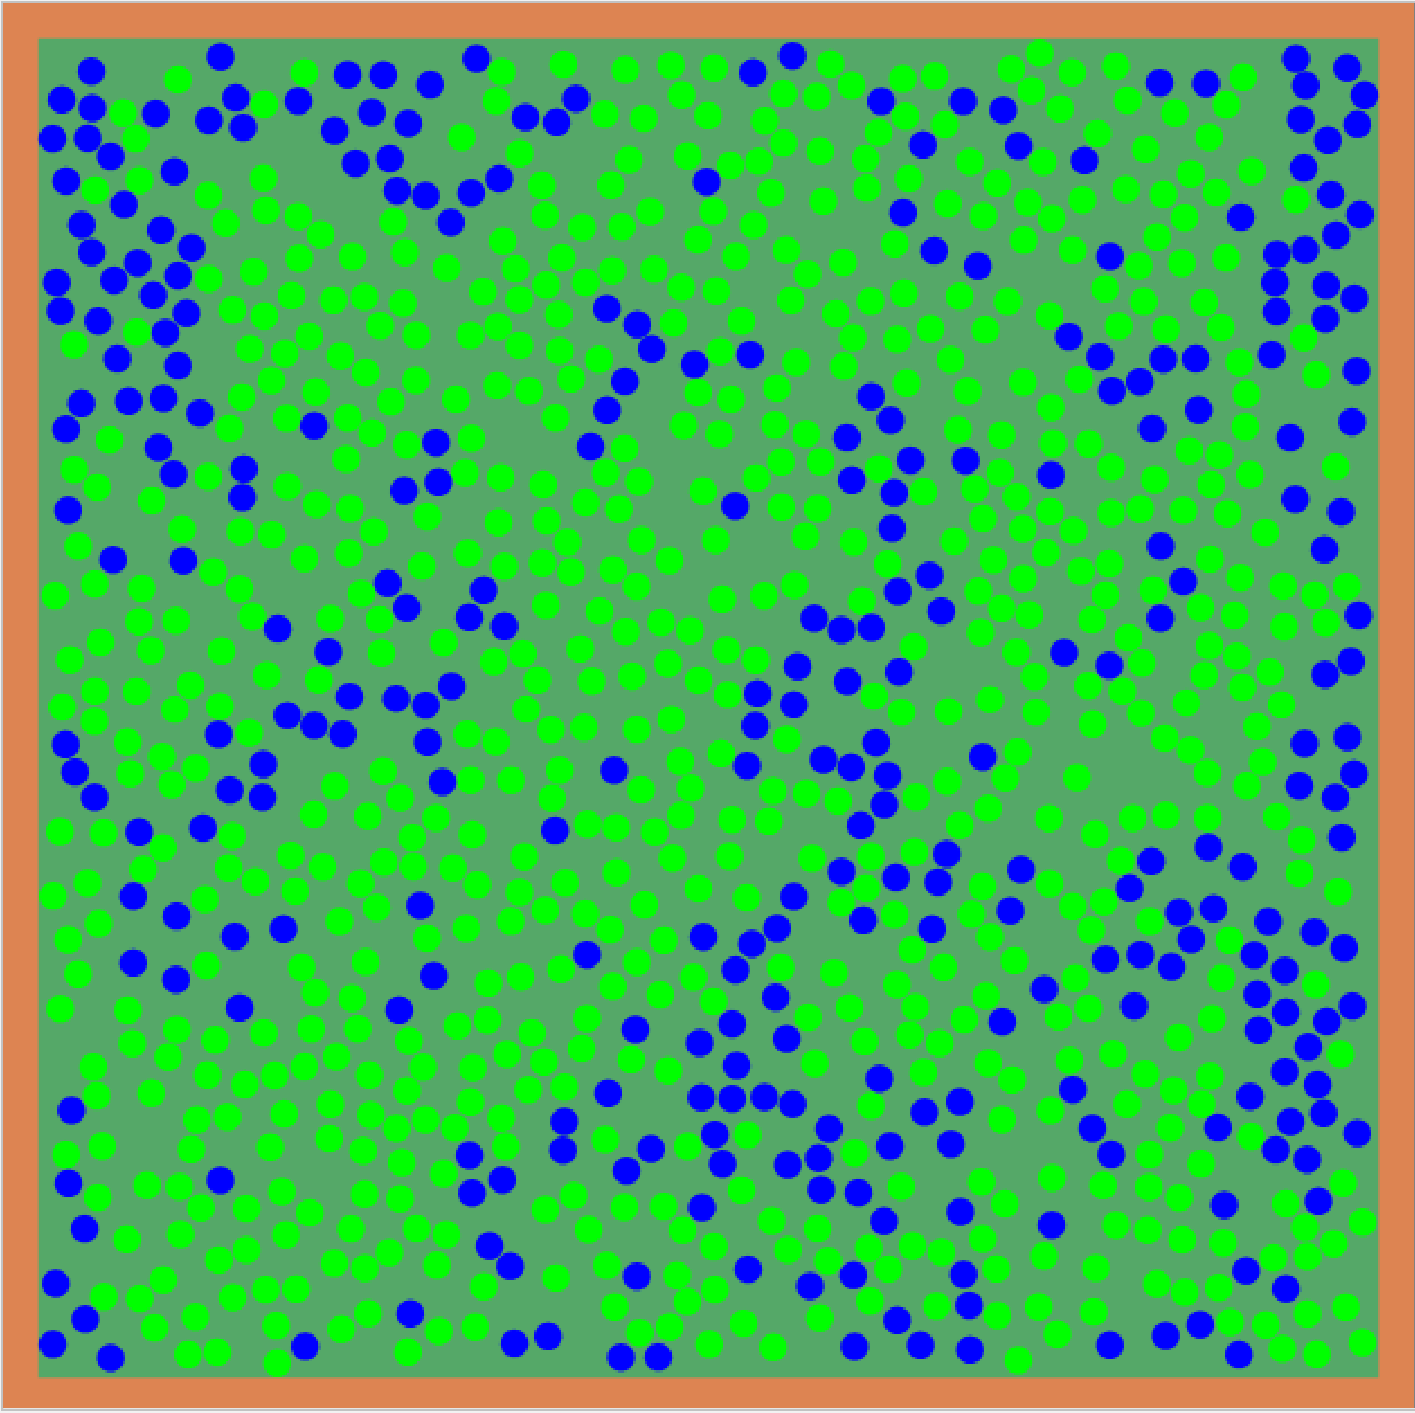
\includegraphics[width=0.8\textwidth]{images/2-51b.png}
     \caption{I: 0.1 - R: 0.2}
     \label{fig: 51b}
 \end{subfigure}
 \begin{subfigure}[b]{0.4\textwidth}
      \centering
     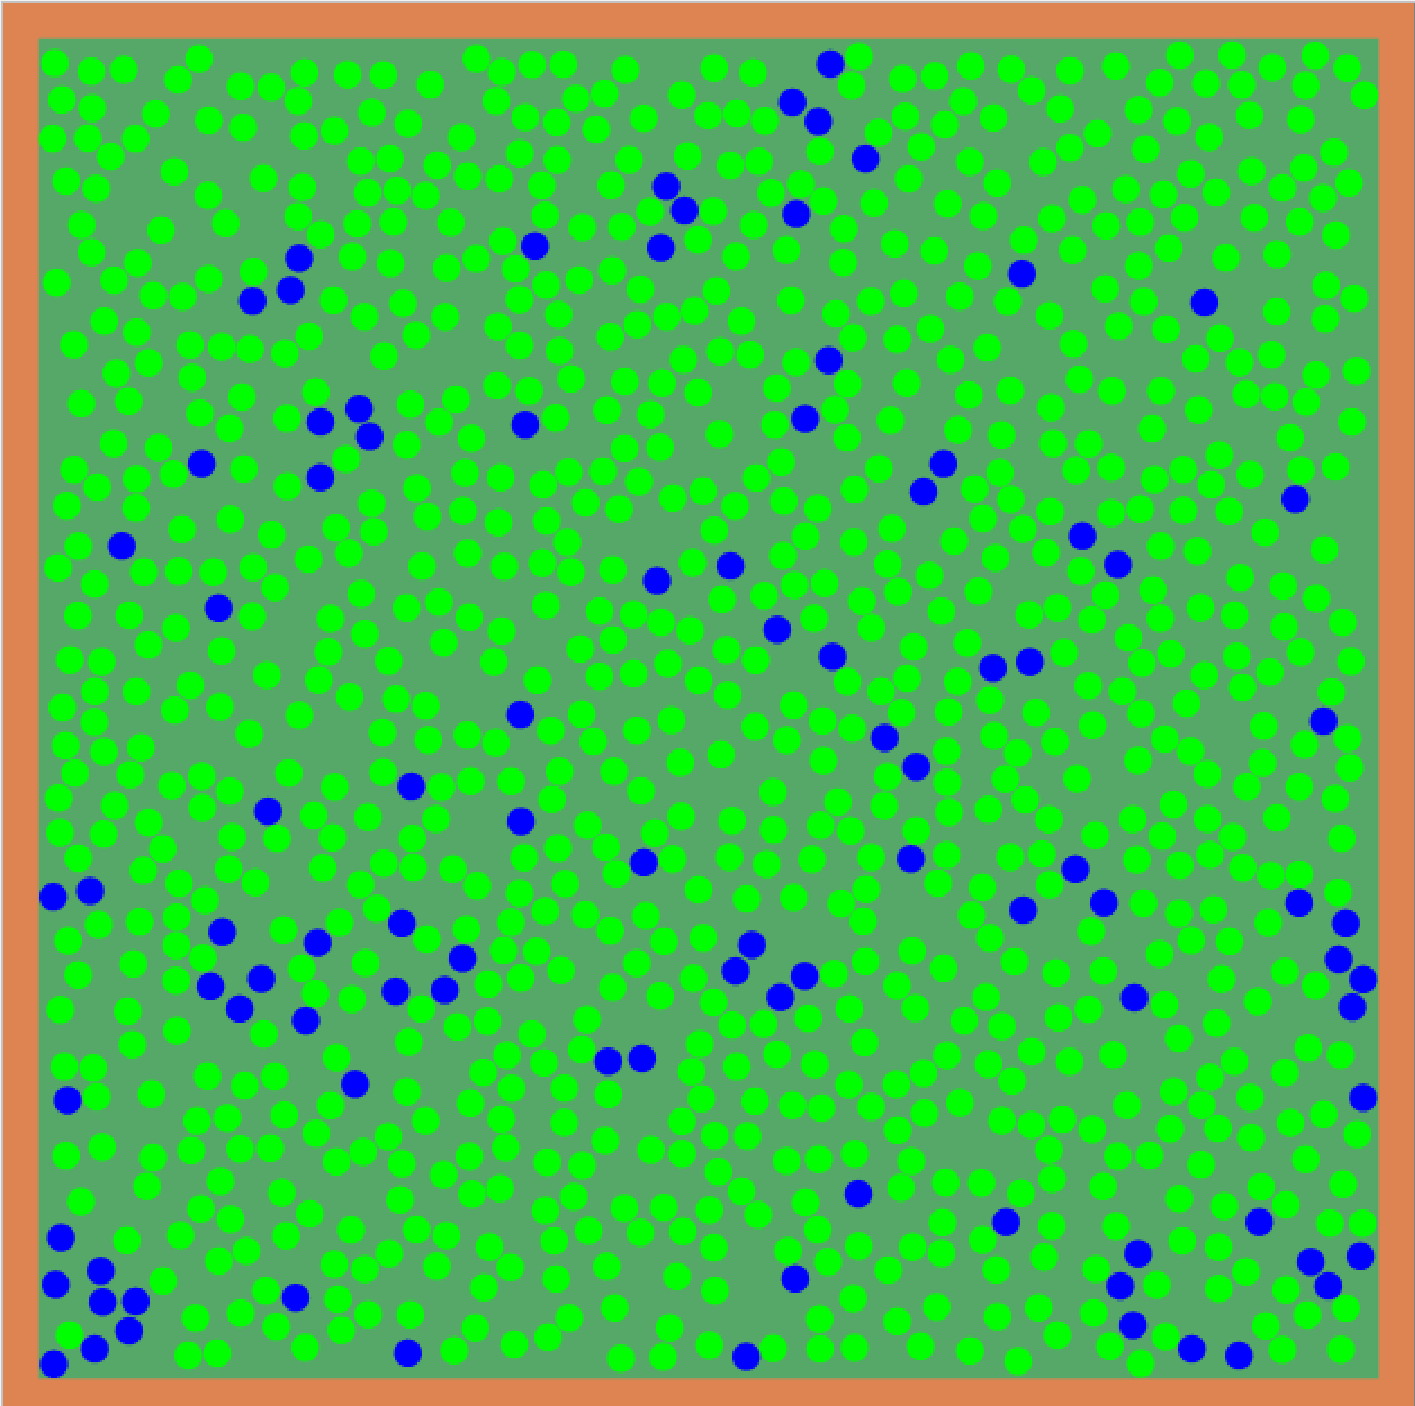
\includegraphics[width=0.8\textwidth]{images/2-51c.png}
     \caption{I: 0.1 - R: 0.1}
     \label{fig: 51c}
 \end{subfigure}
 \begin{subfigure}[b]{0.4\textwidth}
      \centering
     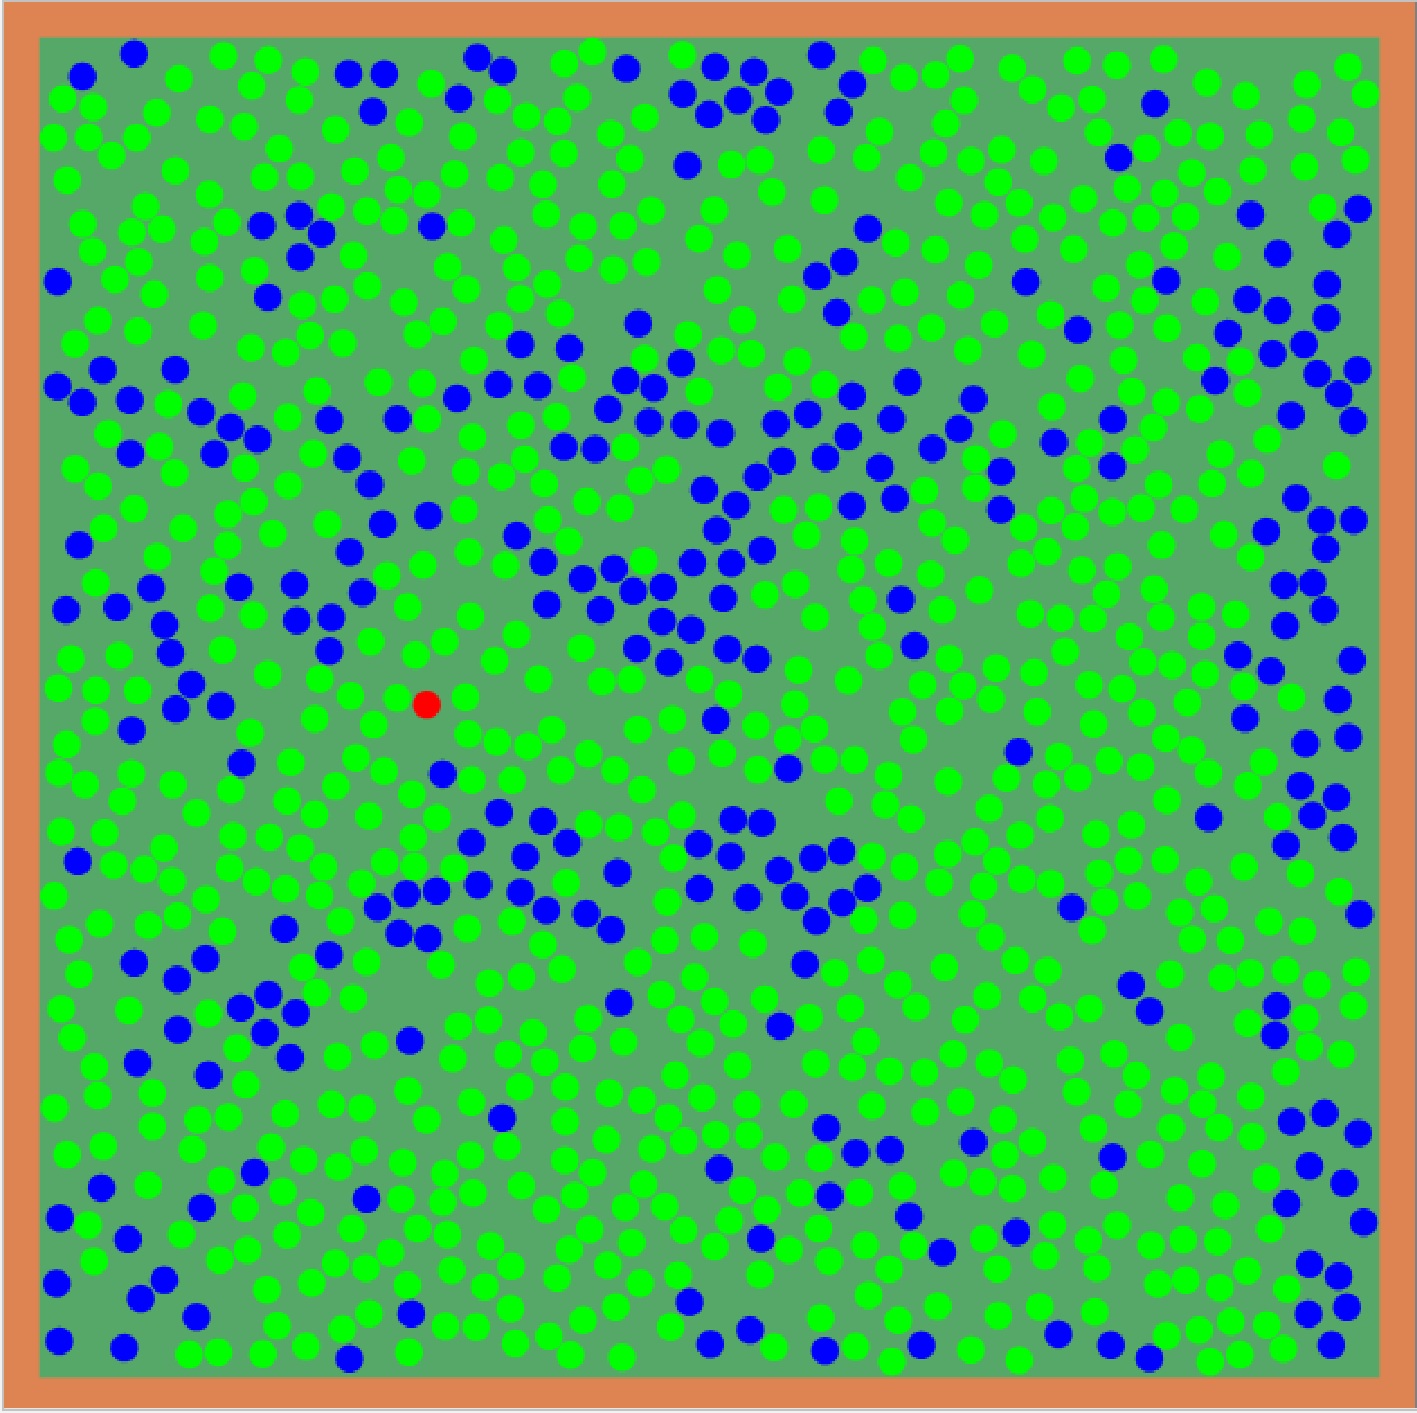
\includegraphics[width=0.8\textwidth]{images/2-51d.png}
     \caption{I: 0.05 - R: 0.1}
     \label{fig: 51d}
 \end{subfigure}
 \caption{Final simulation picture for different infection (I) and recovery (R) rates}
 \label{fig: 51ad}
\end{figure}

\begin{figure}[H]
 \centering
 \begin{subfigure}[b]{\textwidth}
     \centering
     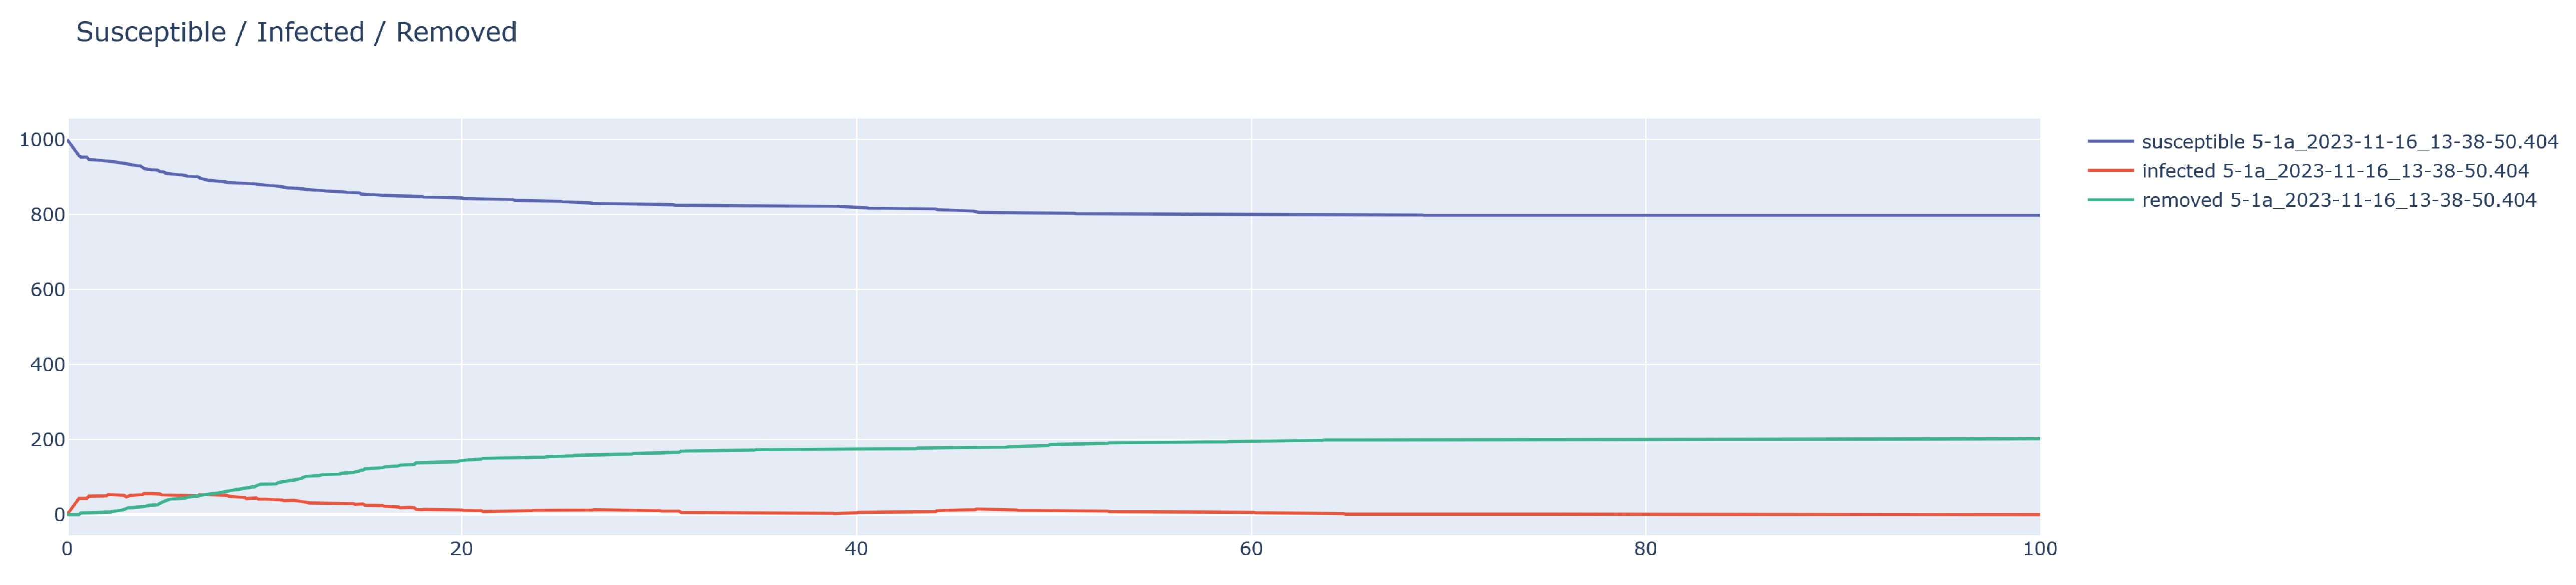
\includegraphics[width=\textwidth]{images/2-5a.png}
    \caption{I: 0.05 - R: 0.2}
    \label{fig: 5a}
 \end{subfigure}
 \begin{subfigure}[b]{\textwidth}
      \centering
     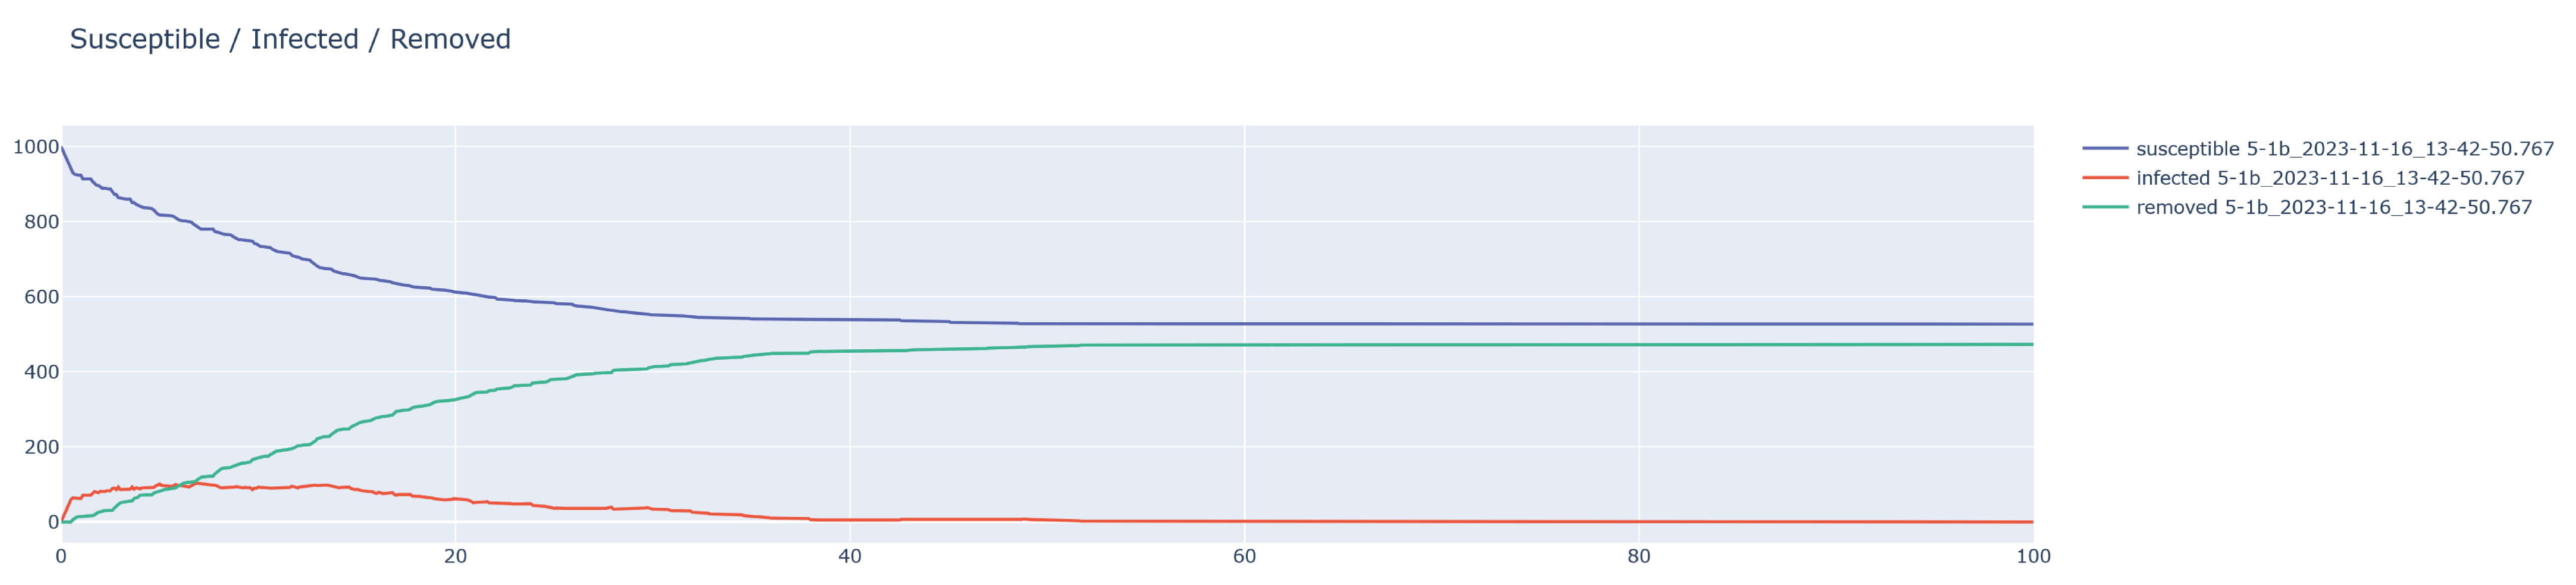
\includegraphics[width=\textwidth]{images/2-5b.png}
     \caption{I: 0.1 - R: 0.2}
     \label{fig: 5b}
 \end{subfigure}
 \begin{subfigure}[b]{\textwidth}
      \centering
     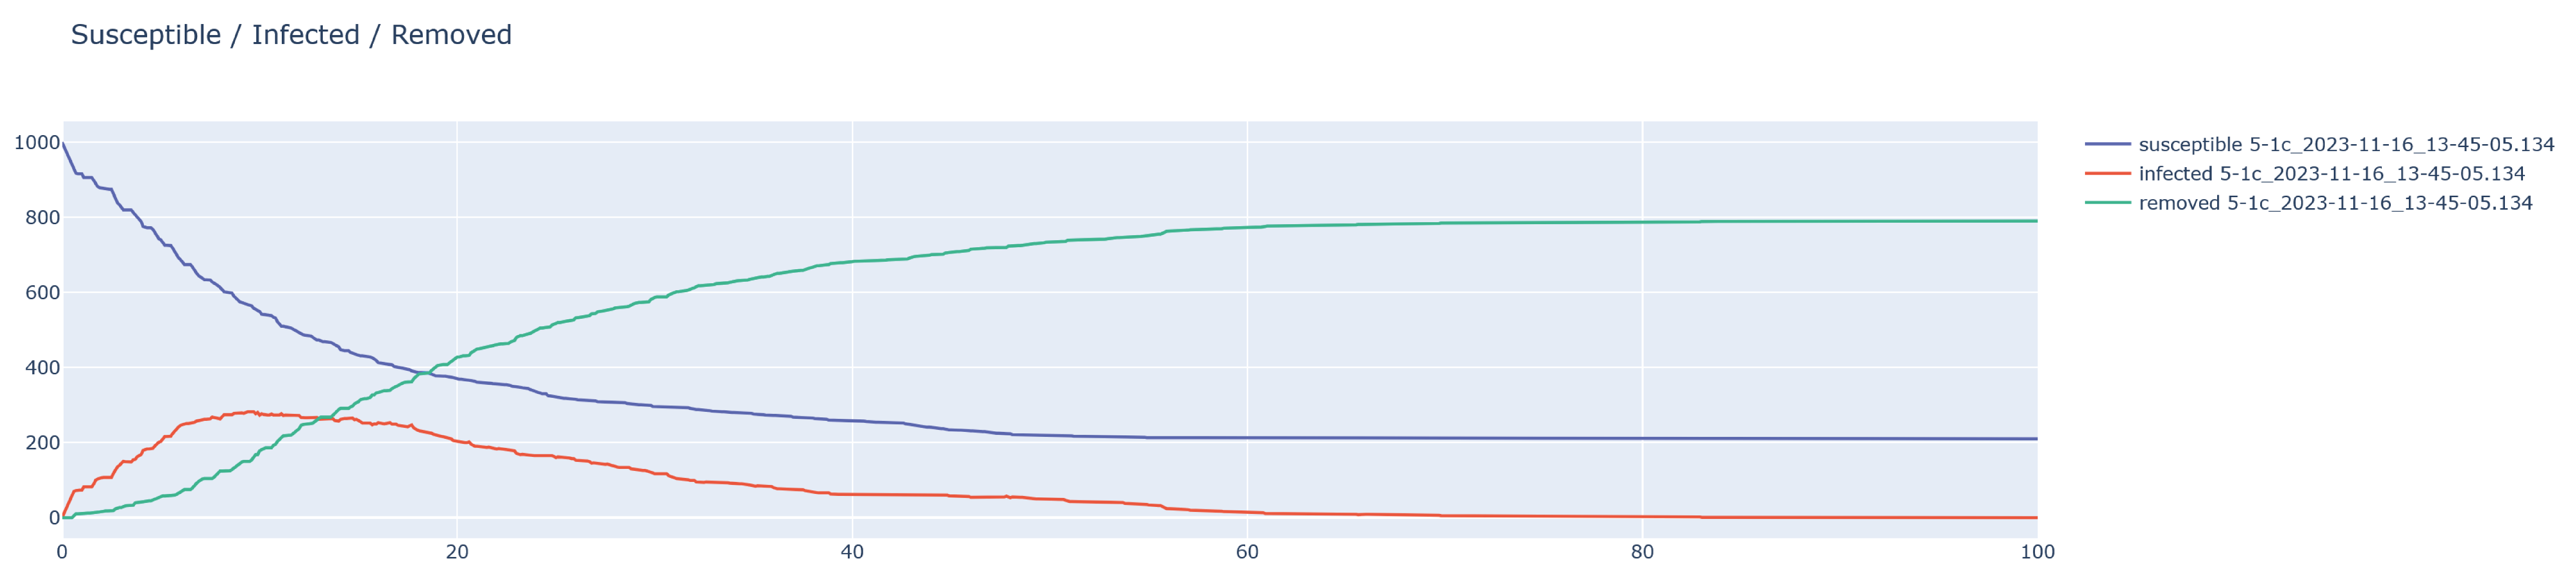
\includegraphics[width=\textwidth]{images/2-5c.png}
     \caption{I: 0.1 - R: 0.1}
     \label{fig: 5c}
 \end{subfigure}
 \begin{subfigure}[b]{\textwidth}
      \centering
     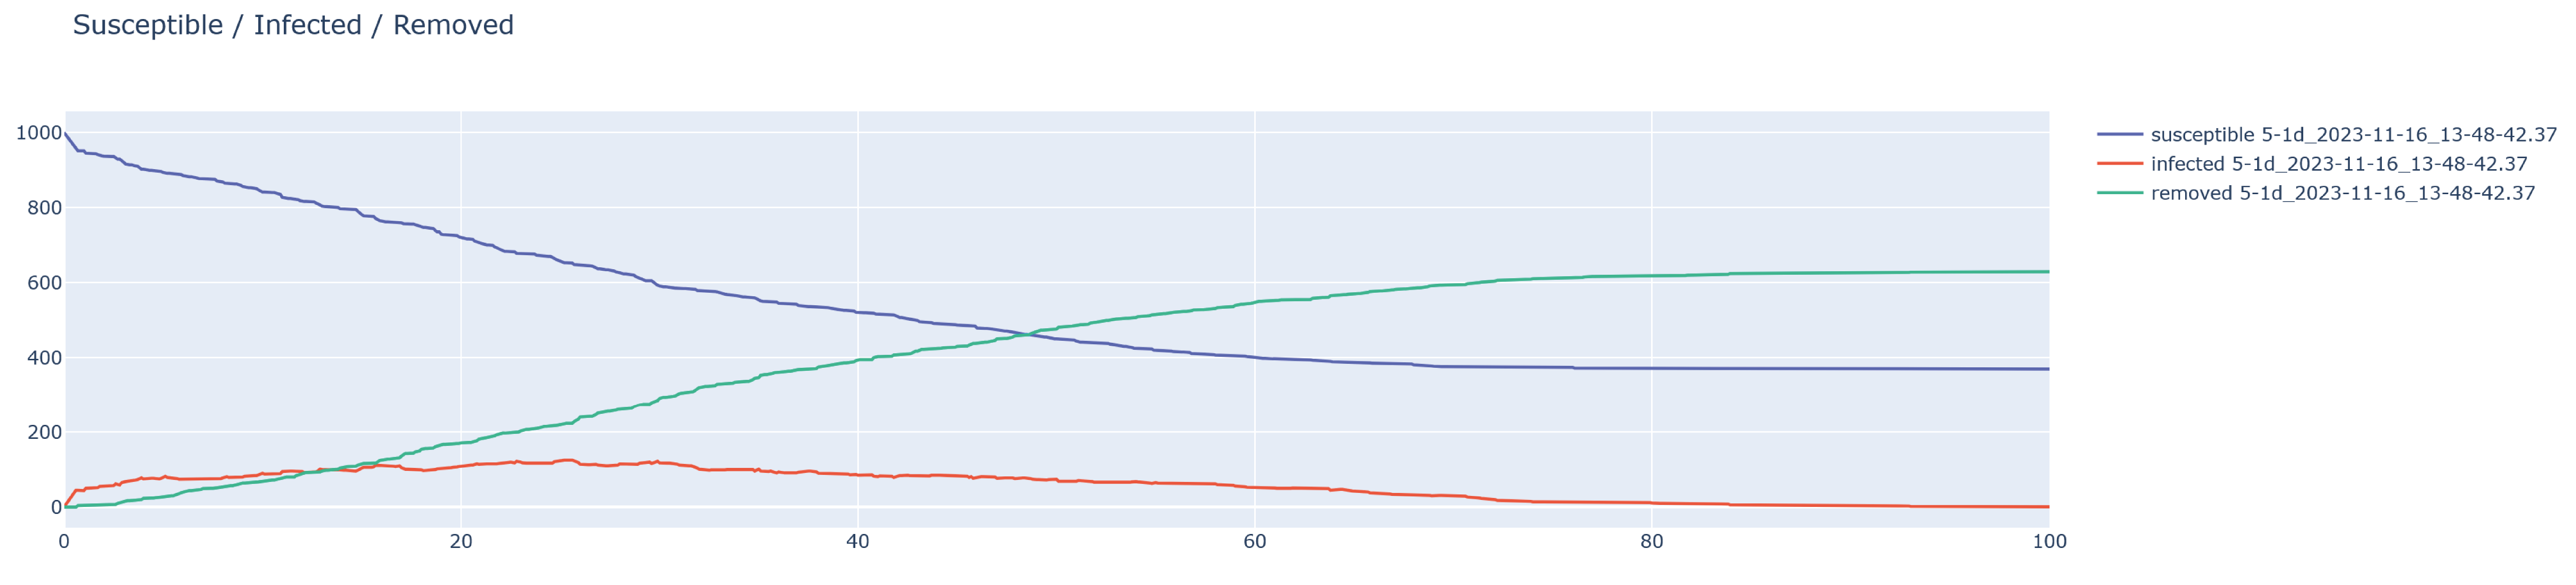
\includegraphics[width=\textwidth]{images/2-5d.png}
     \caption{I: 0.05 - R: 0.1}
     \label{fig: 5d}
 \end{subfigure}
 \caption{Comparison of different infection (I) and recovery (R) rates}
 \label{fig: 5ad}
\end{figure}

\textit{\textbf{Supermarket simulation}}

To create a fairly realistic scenario of a supermarket, we took inspiration from the supermarket model available on \href{https://www.smartdraw.com/store-layout/examples/grocery-store-layout/}{smartdraw}. To comply with the requirement of having a supermarket of at least 30x30m, however, all dimensions have been roughly doubled compared to the previous model, which may affect the realism of the simulation.

\begin{figure}[H]
    \begin{subfigure}[b]{0.49\textwidth}
        \centering
        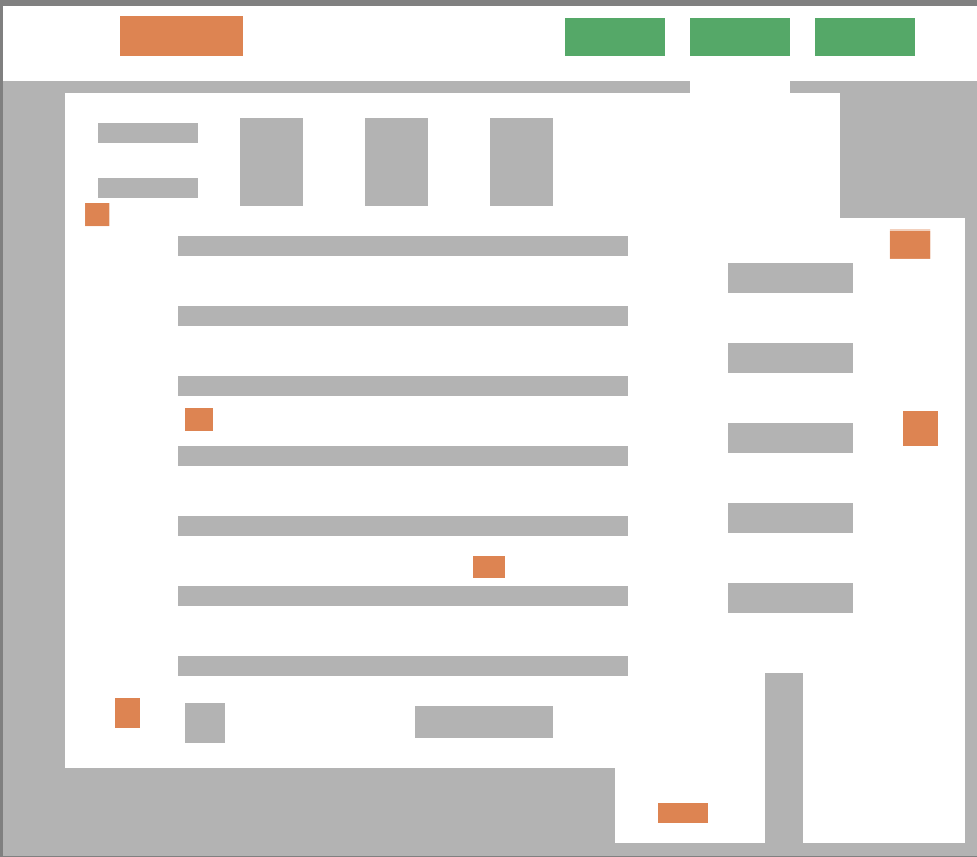
\includegraphics[width=\textwidth]{images/supermarket_design.png}
        \caption{Supermarket model}
        \label{fig:supermarket_a}
    \end{subfigure}
    \hfill
    \begin{subfigure}[b]{0.49\textwidth}
        \centering
        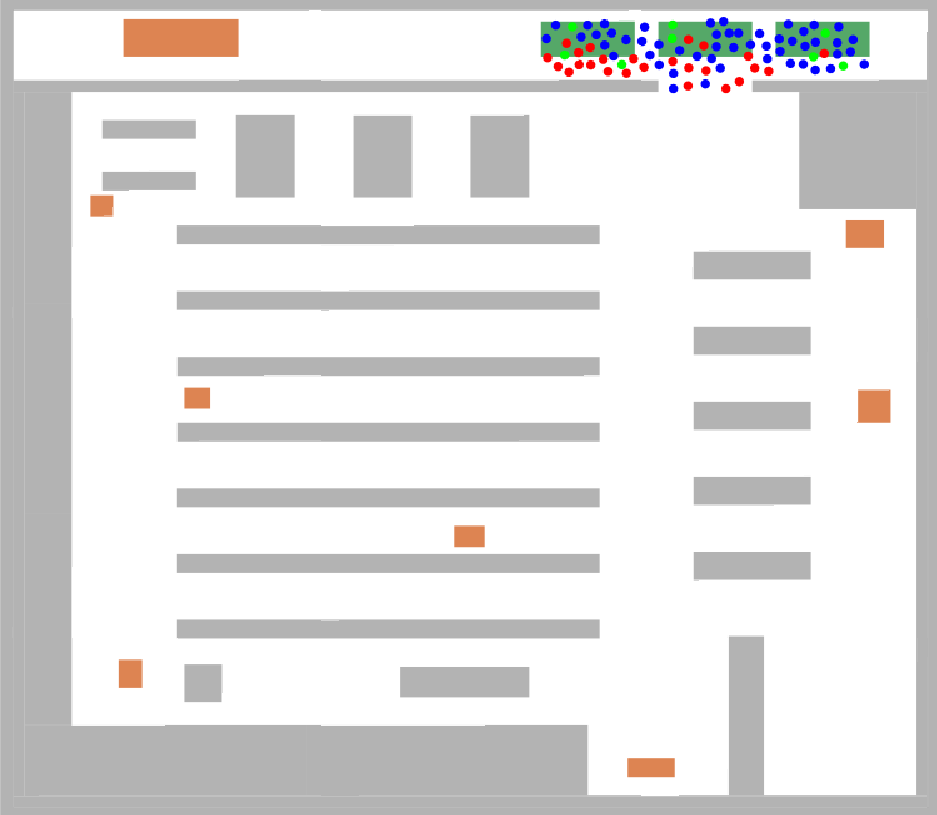
\includegraphics[width=\textwidth]{images/task5_shoppingbegin.png}
        \caption{Pedestrians enter the supermarket}
        \label{fig:supermarket_b}
    \end{subfigure}

    \begin{subfigure}[b]{0.49\textwidth}
        \centering
        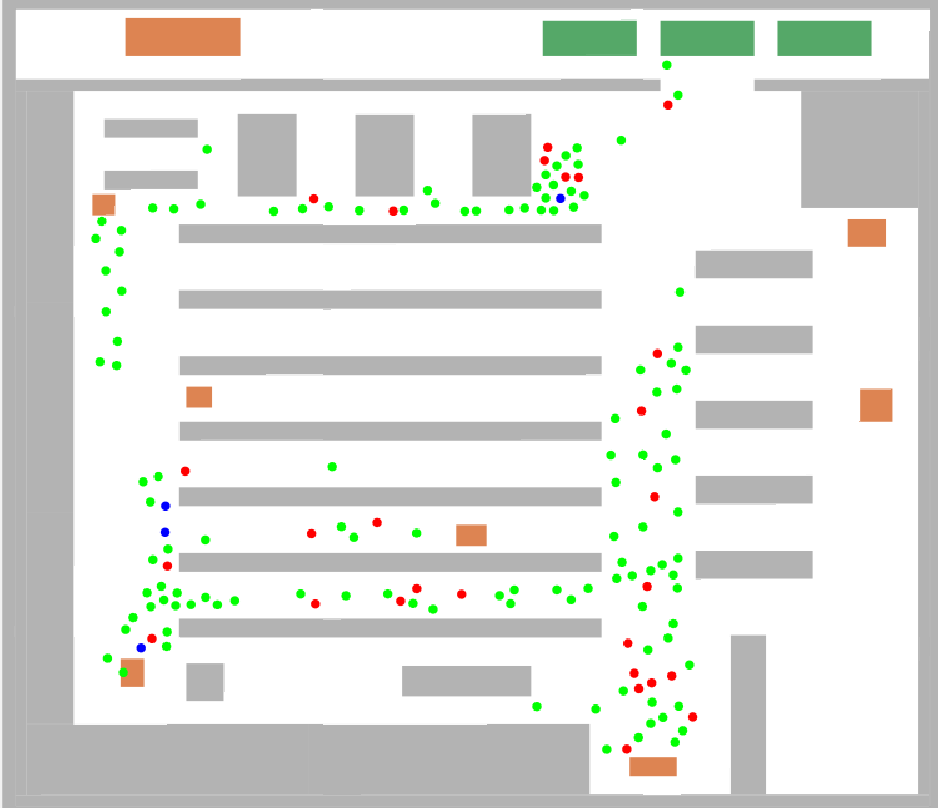
\includegraphics[width=\textwidth]{images/task5_shoppingmid.png}
        \caption{ Pedestrians are walking around the supermarket}
        \label{fig:supermarket_c}
    \end{subfigure}
    \hfill
    \begin{subfigure}[b]{0.49\textwidth}
        \centering
        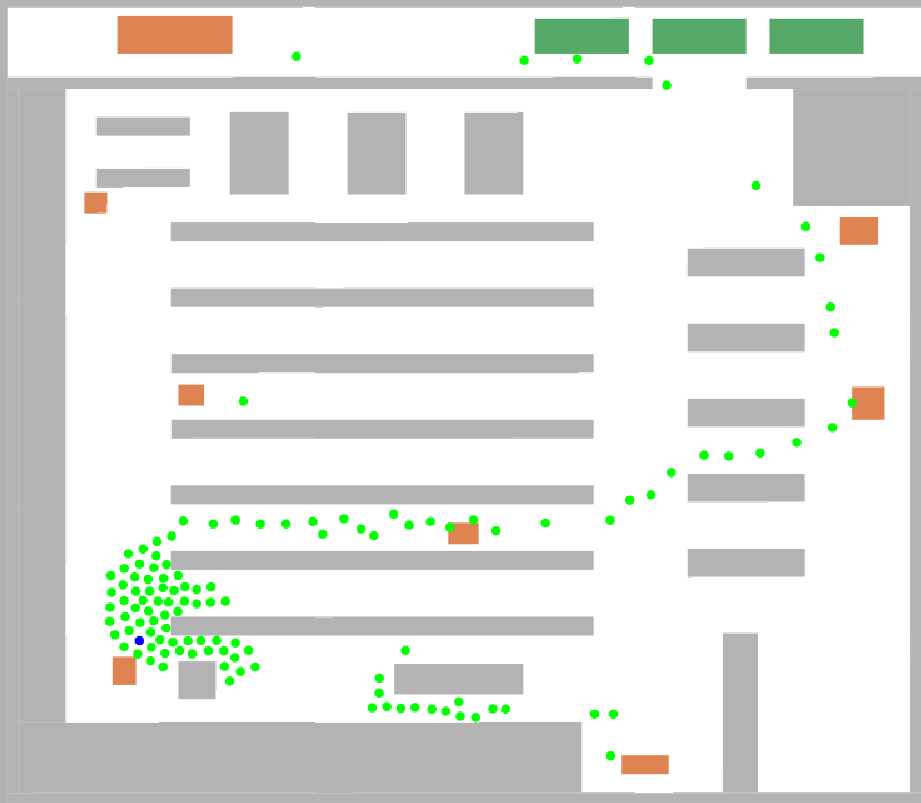
\includegraphics[width=\textwidth]{images/task5_shoppingend.png}
        \caption{Some pedestrians are returning however, some of them are stuck inside of a crowd}
        \label{fig:supermarket_d}
    \end{subfigure}
\caption{Supermarket Scenario for $\texttt{pedPotentialPersonalSpaceWidth} = 0.5$ }
    
\end{figure}

To get pedestrians to take different paths, 3 sources of 50 pedestrians have been implemented (150 in total for the scenarios), each group having different target orders (routings) inside the supermarket before leaving. 
For all the scenarios, the following parameters are fixed and set:
\begin{itemize}
    \item \texttt{infectionsAtStart} : 10 
    \item \texttt{infectionRate} : 0.1
    \item \texttt{infectionMaxDistance} : 1.0
    \item \texttt{recoveredfixedRate} : 0.05
\end{itemize}

To see what happens when increasing the \texttt{pedPotentialPersonalSpaceWidth}, 4 tests have been implemented with different values for this parameter: 0.5, 1.5, 2.5, and 3.5. 

Regarding the paths of the pedestrians, we notice the following during the scenarios: the lower the value of \texttt{pedPotentialPersonalSpaceWidth} is, the more they get stuck in the corridors as different pedestrians headed in different directions hinder each other's motion. Some pedestrians even cannot complete their objective in a time frame of 500 seconds.\\

Regarding the spread of the infection, referring to the SIR visualisations, 
both 0.5 (see figure \ref{fig:t5-s1}) and 1.5 (see figure \ref{fig:t5-s2}) meters produce a high initial spike in infections, in which it subsides faster for a value of 1.5. While there is a difference in the total number of infections, it is a rather small amount. Adding another meter to achieve a \texttt{pedPotentialPersonalSpaceWidth} of 2.5 results in a drastic difference, however, as can be seen in figure \ref{fig:t5-s3}. The initial infection spike is less than 50, and the line of susceptible and removed pedestrians does not intersect, i.e. less than half of the supermarket visitors become infected. Figure \ref{fig:t5-s4} shows an interesting result: The graph does not show even fewer infections like it was to be expected. Despite the efforts to increase the distance between pedestrians, the limited space, particularly at the entrance, leads to crowded conditions, facilitating the transmission of infections. \\

To reduce the number of infections, we want to introduce several ideas: First of all, only a specified amount of pedestrians should be allowed inside a supermarket depending on its size. We made calculations for what could be the best number of people for $\texttt{pedPotentialPersonalSpaceWidth} = 3.5$. It can be seen from figure \ref{fig:graph119}, that when \textbf{119} people were allowed to enter the supermarket, less than 50\% of the people got infected due to a smaller crowd at the entrance.

%will put pitcure
\begin{figure}[H]
    \centering
    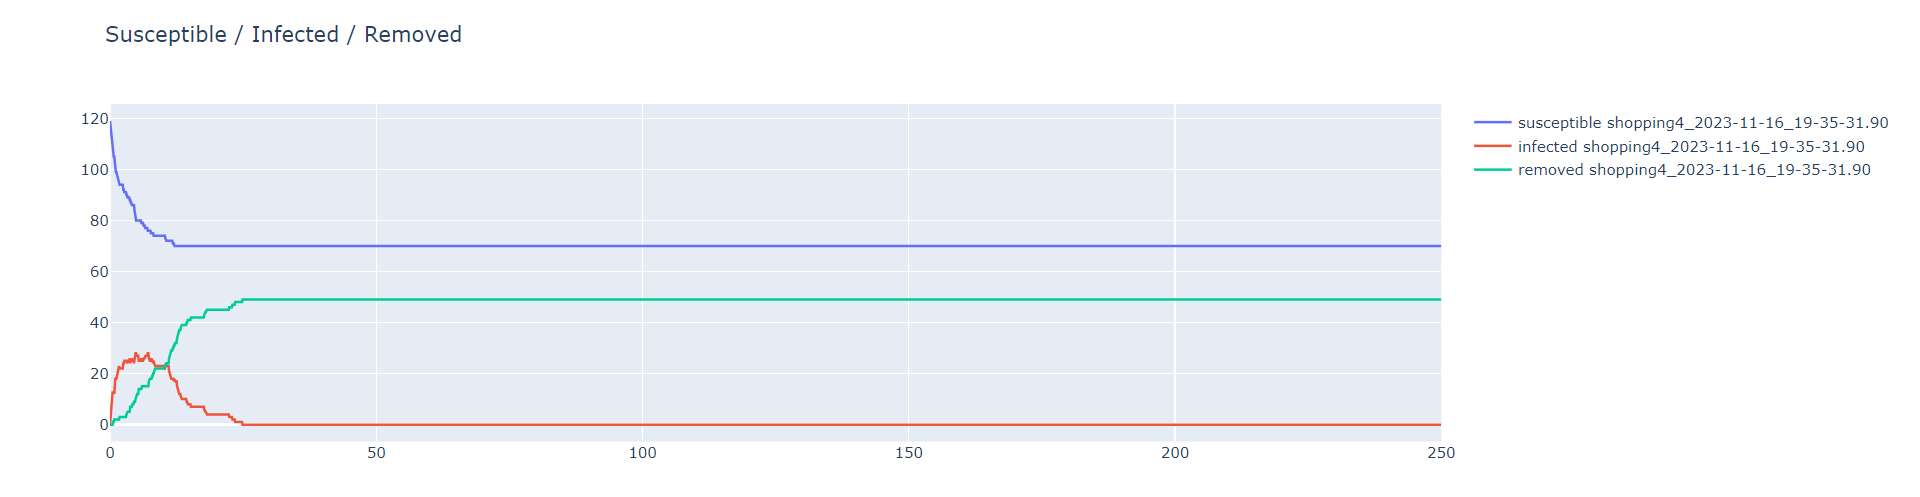
\includegraphics[width=\linewidth]{images/task5_shopping5.png}
    \caption{119 people are allowed to enter the supermarket}
    \label{fig:graph119}
\end{figure}



While waiting outside, the people need to retain distance as well. This can be realized using drawn-on lines in the parking lot as well as using shopping carts for more flexible queues. Both of these methods have been used during the height of the COVID-19 pandemic. \cite{covid-queue-bbc, covoid-queue-wired}


Additionally, specific routes can be marked inside the supermarket to achieve 'one-way streets' to avoid the need to close the gap between pedestrians even for a short amount of time. 


%\begin{center}
\begin{figure}[H]
    \centering
    \begin{subfigure}[t]{\textwidth}
        \centering
        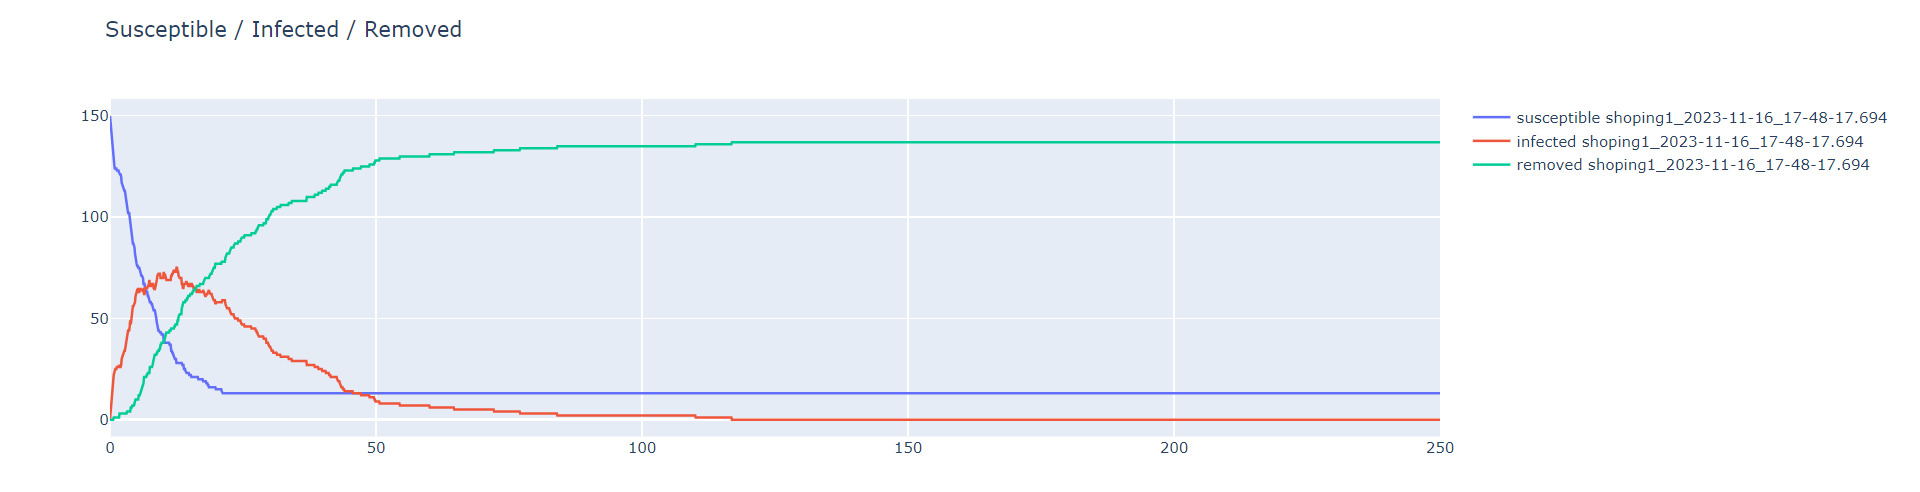
\includegraphics[width=\linewidth]{images/task5_shopping1.png}
        \caption{\texttt{pedPotentialPersonalSpaceWidth} = 0.5}
        \label{fig:t5-s1}
    \end{subfigure}%

    \begin{subfigure}[t]{\textwidth}
        \centering
        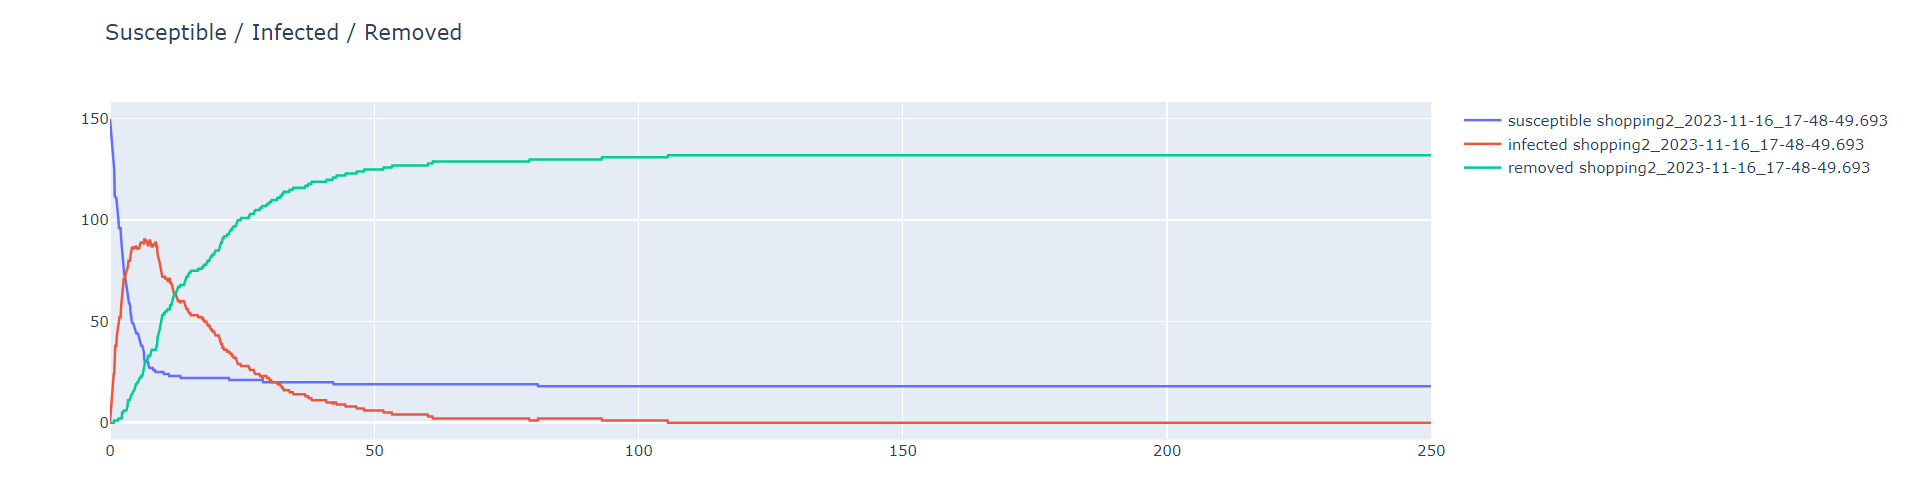
\includegraphics[width=\linewidth]{images/task5_shopping2.png}
        \caption{\texttt{pedPotentialPersonalSpaceWidth} = 1.5}
        \label{fig:t5-s2}
    \end{subfigure}

    \centering
    \begin{subfigure}[t]{\textwidth}
        \centering
        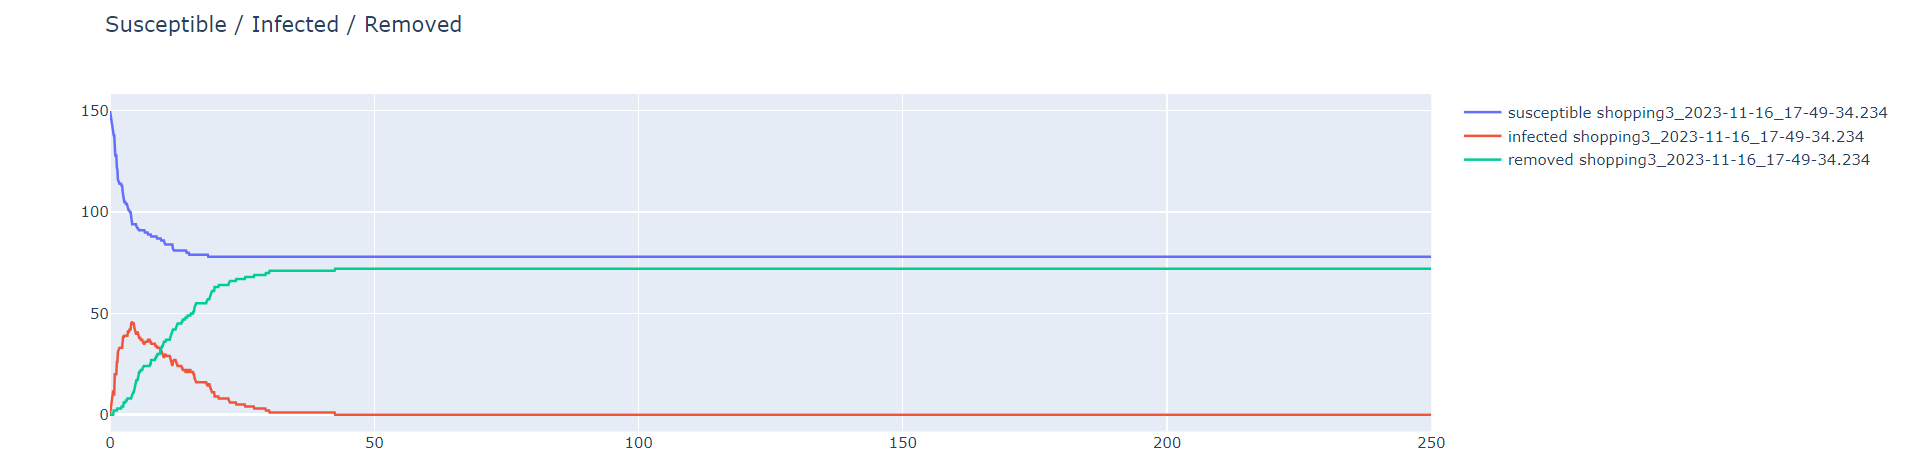
\includegraphics[width=\linewidth]{images/task5_shopping3.png}
        \caption{ \texttt{pedPotentialPersonalSpaceWidth} = 2.5}
        \label{fig:t5-s3}
    \end{subfigure}%
    
    \begin{subfigure}[t]{\textwidth}
        \centering
        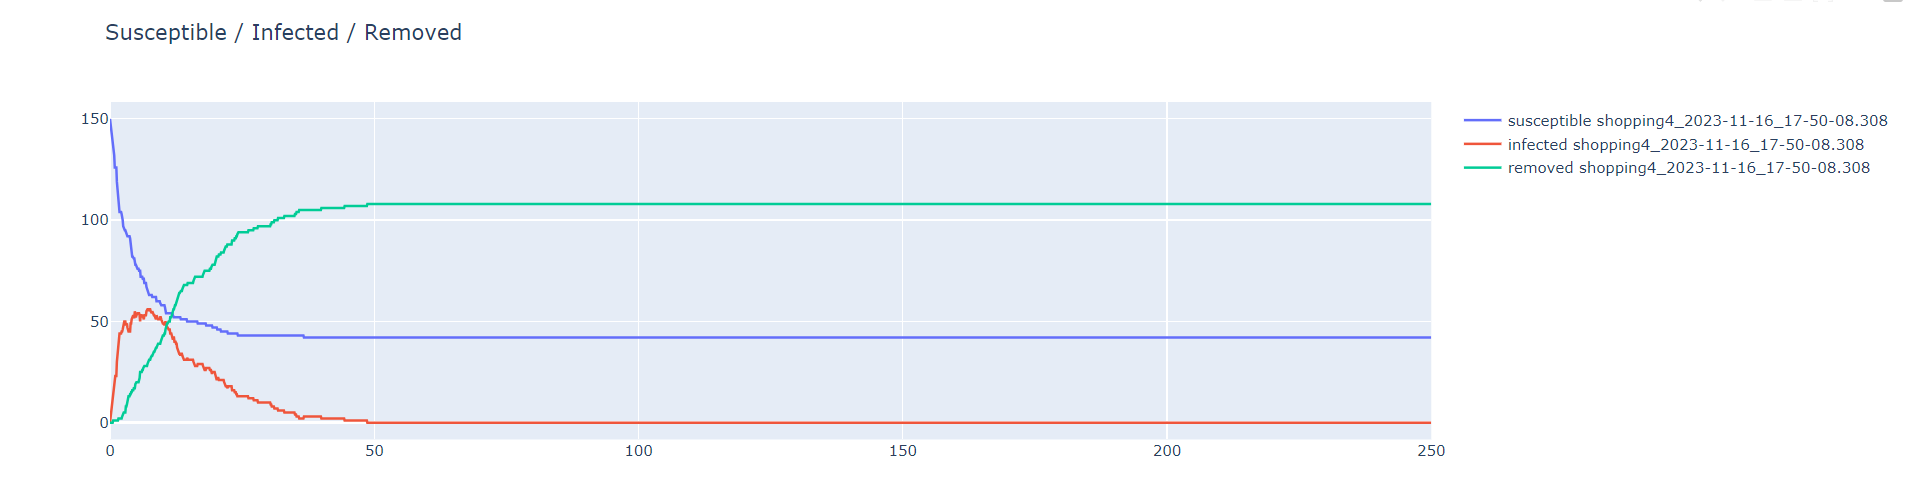
\includegraphics[width=\linewidth]{images/task5_shopping4.png}
        \caption{\texttt{pedPotentialPersonalSpaceWidth} = 3.5}
        \label{fig:t5-s4}
    \end{subfigure}

    \caption{Comparison of different \texttt{pedPotentialPersonalSpaceWidth} in market scenario}
\end{figure}
\end{task}

\bibliographystyle{plain}
\bibliography{Literature}

\end{document}